\documentclass[
        12pt,
        openany, %openright,			
        oneside, %twoside,
        a4paper,			
        english,			
        brazil
        ]{abntbibufjf}

\usepackage{lmodern}						
\usepackage[T1]{fontenc}		
\usepackage[utf8]{inputenc}	

\usepackage{amsmath,amsthm,latexsym,amsbsy}

\usepackage{listings}
\lstset{language=C,
	numbers=left,
	numberstyle=\footnotesize,
	frame=single,
	showstringspaces=false
}


\usepackage{lastpage}			
\usepackage{indentfirst}
\usepackage{color}
\usepackage{graphicx}			
\usepackage{microtype}

\usepackage{hyperref}	

\graphicspath{{img/}}



\usepackage{tikz}
\usetikzlibrary{shapes,arrows}
\usepackage{circuitikz}

\usepackage{ulem}

\usepackage{pdfpages}

\titulo{Driver de Dois Estágios para Acionamento \\ de LEDs de Extra-Alta Corrente} 
\autor{Eric Pusiol}
\autorR{Pusiol, Eric}
\local{Juiz de Fora}
\data{Dezembro, 2019}
\orientador[Orientador:]{Henrique Antônio Carvalho Braga}
\coorientador[Coorientador:]{Denis de Castro Pereira}
\instituicao{Universidade Federal de Juiz de Fora}
\faculdade{Faculdade de Engenharia}
\programa{Graduação em Engenharia Elétrica}
\objeto{Trabalho final de curso (Graduação)}
\natureza{Trabalho final de curso
apresentado à \inserefaculdade ~da Universidade Federal de Juiz de Fora, na área de concentração em eletrônica de potência, como requisito parcial para obtenção do título de Engenheiro Eletricista.}


%% Abaixo, prencher com os dados da parte final da ficha catalografica

\finalcatalog{Iluminação. COB LED. Alto fluxo luminoso. Driver de dois estágios. Modo de condução contínua. I. Braga, Henrique Antônio Carvalho, orient. II. Pereira, Denis de Castro, coorient. III. Título.} 

%% ---

\setlength{\parindent}{1.3cm}

\setlength{\parskip}{0.2cm}  

\setlength\afterchapskip{12pt}  




\def\antenna{%
	-- +(0mm,4.0mm) o +(2.625mm,7.5mm) -- +(-2.625mm,7.5mm) -- +(0mm,4.0mm)
}

\def\ground{%
	-- +(0mm,-4.0mm) {
		[yshift=-4mm]
		+(-2mm,0mm) -- +(2mm,0mm)
		+(-1mm,-1mm) -- +(1mm,-1mm)
		+(-0.3mm,-2mm) -- +(0.3mm,-2mm)
	}
}




\begin{document}

%% ELEMENTOS PRE-TEXTUAIS

%% Capa
\inserecapa

%% Folha de rosto
\inserefolhaderosto


%% Ficha catalografica. AO IMPRIMIR, DEIXAR NO VERSO DA FOLHA DE ROSTO.
\inserecatalog  


%%%%%%%%%%%%%%%%%%%%%%%%%%%%%%%%%%%%%%%%%%%%%%%%%%%%%%
%% Folha de aprovacao
%\ begin{folhadeaprovacao}

%  \begin{center}
%    {\chapterfont \bfseries \insereautor}

%    \vfill
%    \begin{center}
%      {\chapterfont\bfseries\inseretitulo \inseresubtitulo}
%    \end{center}
%    \vfill
    
%    \hspace{.45\textwidth}
%    \begin{minipage}{.5\textwidth}
%        \inserenatureza
%    \end{minipage}%
%    \vfill
%   \end{center}
        
%   Aprovada em 18 de dezembro de 2019.
   
%   \begin{center} BANCA EXAMINADORA \end{center}
%   \assinatura{Dr. \insereorientador \ - Orientador \\ Universidade Federal de Juiz de Fora}

%   \assinatura{Dr. \inserecoorientador \\ Universidade Federal de Juiz de Fora}
%   \assinatura{Dr. Guilherme Márcio Soares \\ Universidade Federal de Juiz de Fora} 
%
%\end{folhadeaprovacao}
%%%%%%%%%%%%%%%%%%%%%%%%%%%%%%%%%%%%%%%%%%%%%%%%%%%%%%
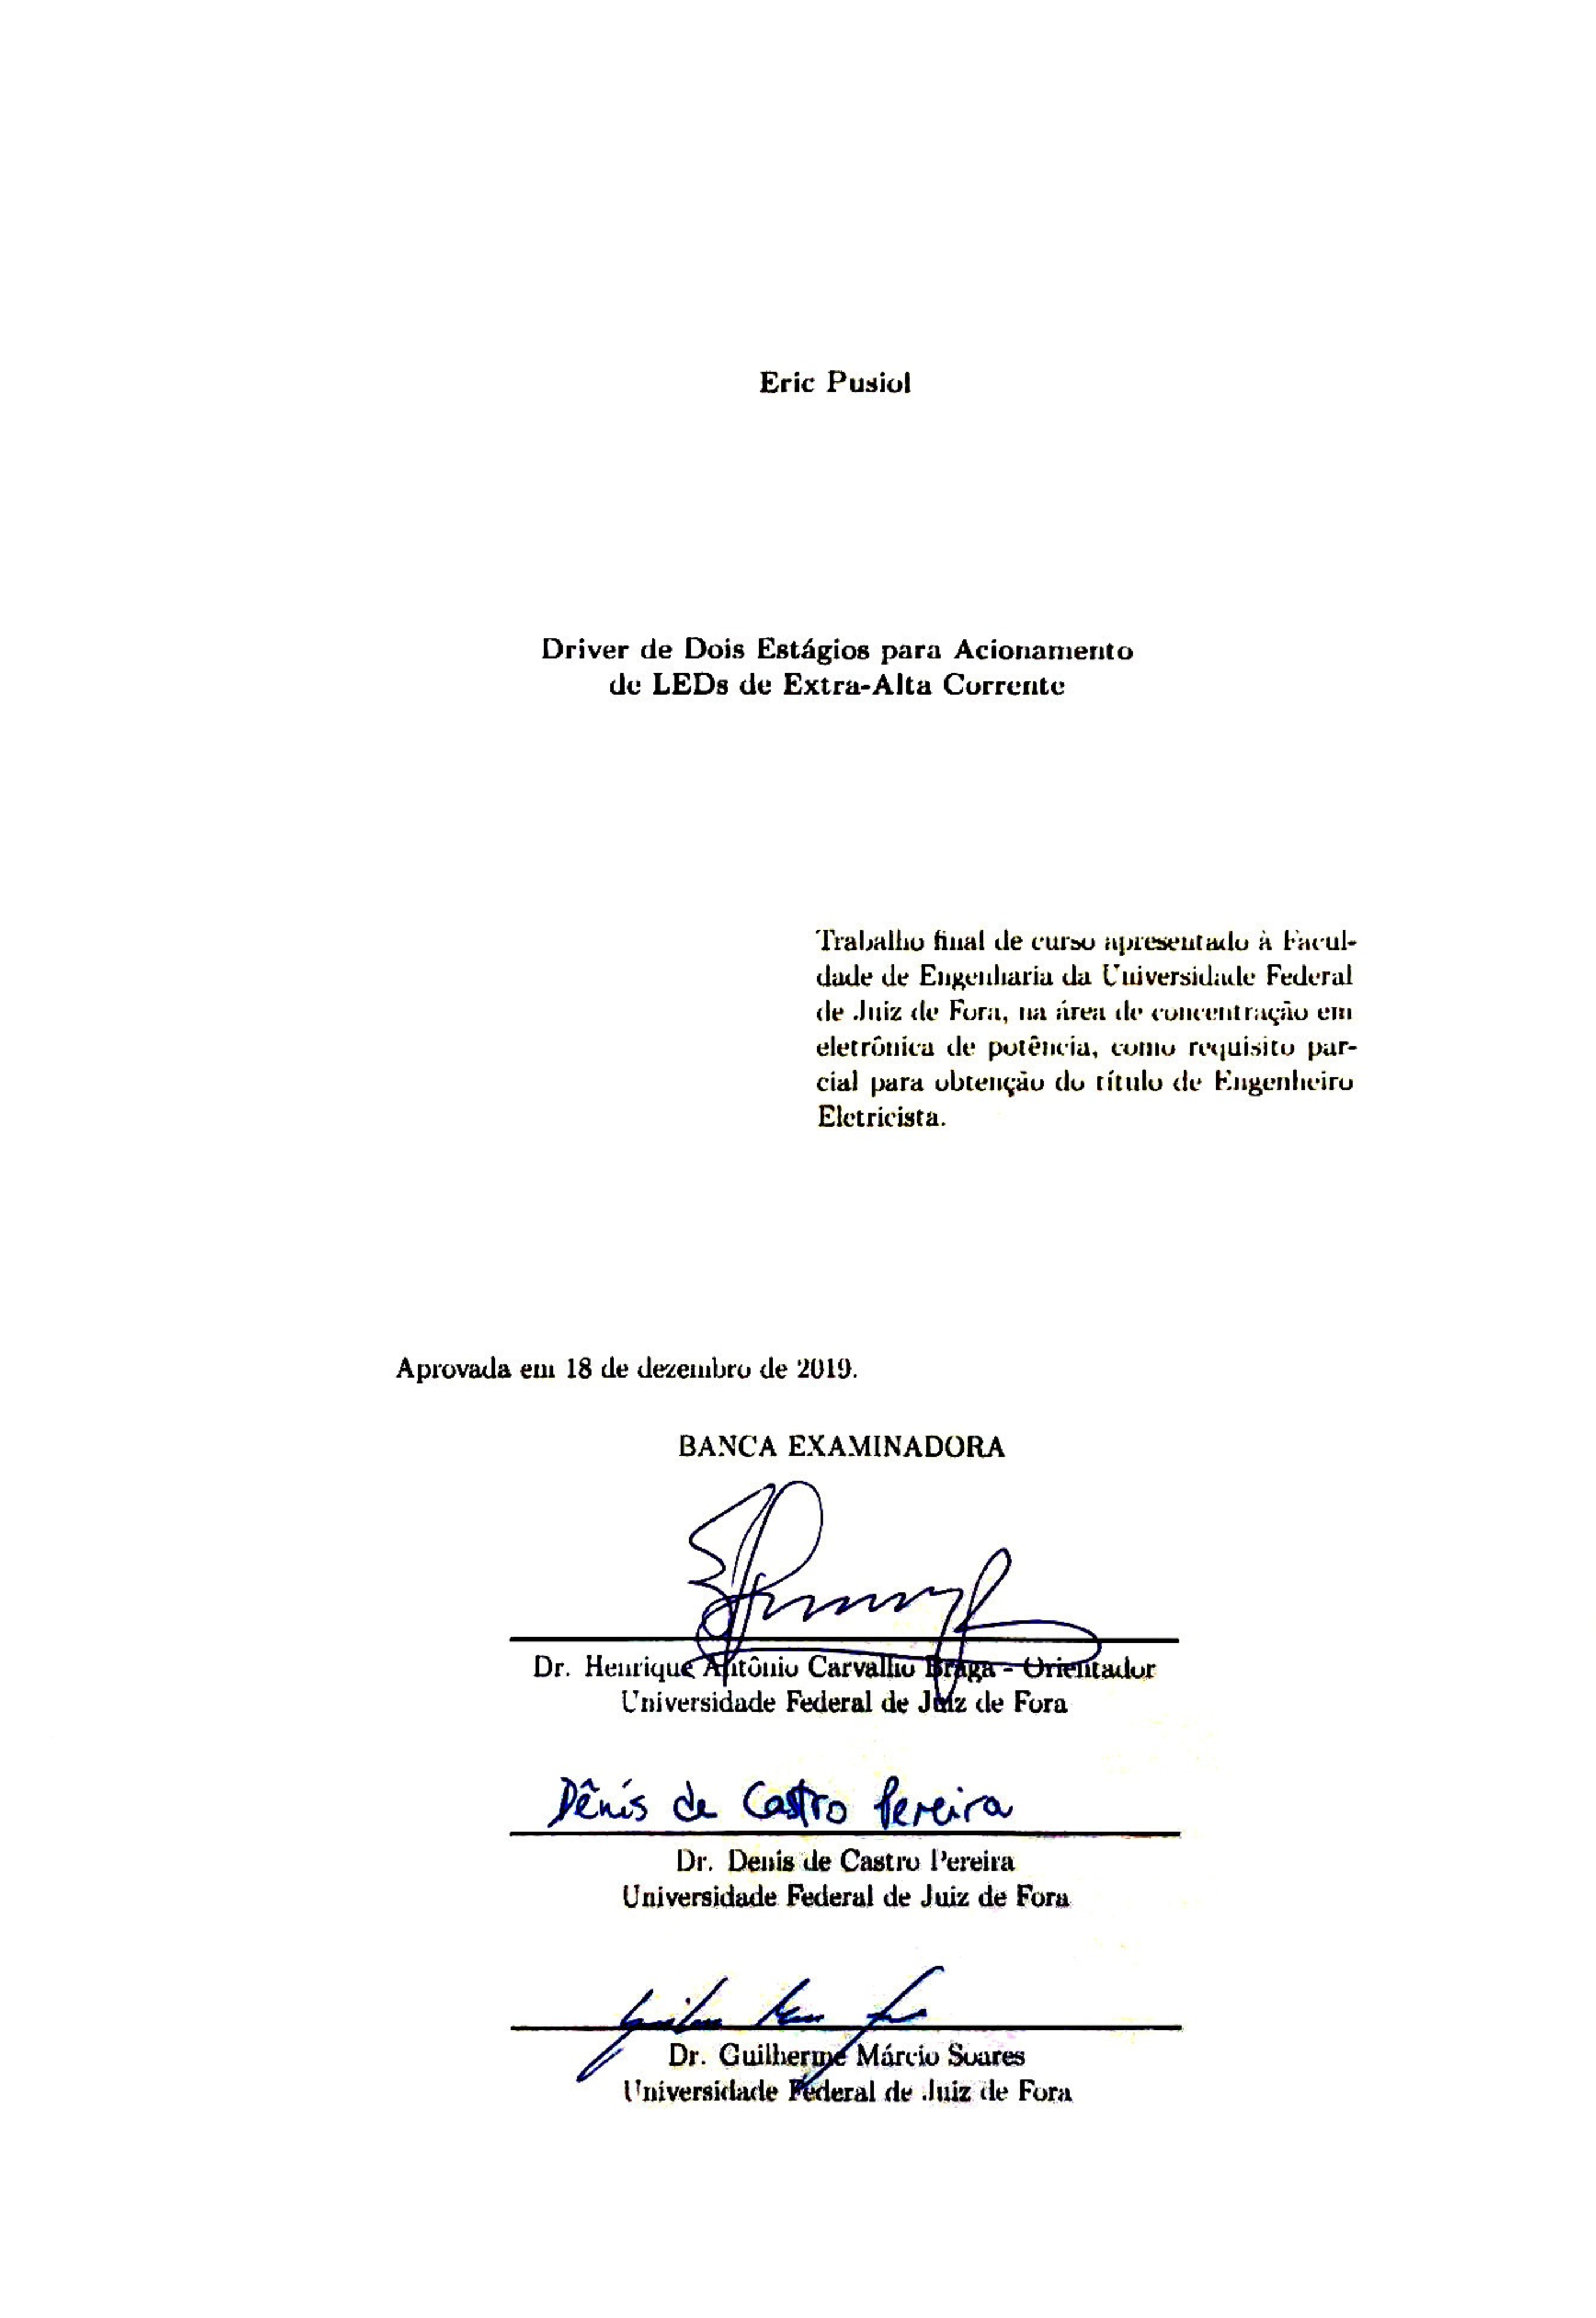
\includepdf[pages=-]{img/fl.pdf}



\begin{agradecimentos}

Agradeço primeiramente a Deus, por tudo o que me deu e me permitiu fazer. Agradeço a minha família, por todo o apoio durante o curso. Agradeço à universidade e seu corpo docente, por ter possibilitado minha formação, aos amigos que estiveram comigo nessa jornada, agradeço ao grupo de pesquisa do NIMO e ao CNPq por ter me dado oportunidade, desafios e meios para a concretização deste trabalho, e a meus orientadores, Henrique Braga e Dênis de Castro, por me darem a direção para a qual navegar. A todos que fizeram parte da minha formação, aqui constados ou não, deixo meu muito obrigado.

%Agradeço sinceramente a Dênis e Braga pela oportunidade, à galera do Nimo pelo apoio, à Capes pela bolsa, à minha família, meus amigos, ao exército brasileiro por ter mantido a paz, à CIA pelo financiamento, ao Tony Stark por ter me iludido a fazer engenharia elétrica, à Texas, Epcos, LT e todas as industriais de semicondutoras que cederam amostras para este trabalho e ao cara que fez o aterramento do nimo pelo péssimo trabalho que me roubou alguns dias pensando em problemas etéreos.

%Não tenho capacidade de escrever um agradecimento, Denis. Vou copiar o seu na íntegra depois.

\end{agradecimentos}

%% Epigrafe. OPCIONAL
\begin{epigrafe}
    \vspace*{\fill}
	\begin{flushright}
		Porque pelas tuas palavras serás justificado, e pelas tuas palavras serás condenado.\\
		Mateus 12:37
	\end{flushright}
\end{epigrafe}


%% RESUMOS

%% Resumo em Portugu^es. OBRIGATORIO.
\setlength{\absparsep}{18pt} 
\begin{resumo}
Diante da peculiaridade de alguns tipos de dispositivos LED modernos, faz-se necessária análise criteriosa, dentre as inúmeras configurações diferentes de carga-rede, da melhor alternativa que atenda àquele caso, ponderando qualidade, eficiência, durabilidade e dispendiosidade. Este documento visa desenvolver tal tratamento à família de cargas EHC COB LED, dispositivos altamente compactos, de elevada potência e fluxo luminoso, ainda com tratamento limitado na literatura técnica, relevantes no atual contexto de iluminação moderna devido à pretensão de permear a tecnologia SSL em diferentes nichos ocupados por sistemas de menor desempenho. Dentro do escopo deste trabalho estão o projeto de um \textit{driver} de dois estágios em cascata, isto é, um estágio pré-regulador com correção do fator de potência, o qual tem como saída um barramento CC de tensão elevada, de centenas de volts, e um estágio final responsável pelo controle da corrente de saída no COB LED. Neste contexto, este ensaio visa demonstrar o projeto teórico, construção física e análise experimental do driver proposto, a fim de comprovar a tecnologia e metodologia desenvolvidas.


Palavras-chave: Iluminação. COB LED. Alto fluxo luminoso. Driver de dois estágios. Modo de condução contínua.

\end{resumo}
 
 
%% Resumo em Ingle^s
\begin{resumo}[ABSTRACT]
 \begin{otherlanguage*}{english}
Given the peculiarity of some types of modern LED devices, it is necessary to carefully analyze, among the many different configurations of network-load, the best alternative that meets each case, considering quality, efficiency, durability and cost. This document aims to develop such evaluation to the EHC COB LED family of loads, which concerns highly compact devices, while also performing high power and luminous flux. These modern LEDs still do not present wide treatment in technical literature, as they are highly relevant in modern lighting. This assumption can be also extended to several areas that employs SSL technology, which are nowadays occupied by systems with lower performance. Within the scope of this work it is considered the design of a two-stage cascaded driver, i.e., a power factor corrected pre-regulator stage, which outputs a high voltage DC bus, of the order of 400V, and a final stage responsible for controlling the output current in the COB LED. In this context, this practical implementation aims to demonstrate the theoretical design, physical construction and experimental analysis of the proposed driver, in order to prove the developed technology and methodology.


Key-words: Lighting, COB LED, High luminous flux, Two-stage driver, Continuous conduction mode.
 \end{otherlanguage*}
\end{resumo}

%% Seguindo o mesmo modelo acima, pode-se inserir resumos em outras linguas. 

%% Lista de ilustracoes. OPCIONAL.
\pdfbookmark[0]{\listfigurename}{lof}
\listoffigures*
\cleardoublepage


%% Lista de tabelas. OPCIONAL. Retire o ``%'' de cada das 3 linhas seguintes, caso queira.
% \pdfbookmark[0]{\listtablename}{lot}
% \listoftables*
% \cleardoublepage

%% Lista de abreviaturas e siglas. OPCIONAL
%\begin{siglas} %%ALTERAR OS EXEMPLOS ABAIXO, CONFORME A NECESSIDADE
%  \item[ABNT] Associa\c{c}\~ao Brasileira de Normas T\'ecnicas
%  \item[UFJF] Universidade Federal de Juiz de Fora
%  \item[IBGE] Instituto Brasileiro de Geografia e Estat\'istica
%\end{siglas}

%% Lista de simbolos. OPCIONAL
%\begin{simbolos} %%ALTERAR OS EXEMPLOS ABAIXO, CONFORME A NECESSIDADE
%  \item[$ \forall $] Para todo
%  \item[$ \in $] Pertence
% \end{simbolos}

 
%% Sumario
\pdfbookmark[0]{\contentsname}{toc}
\tableofcontents*
\cleardoublepage

%% ----------------------------------------------------------

%% ELEMENTOS TEXTUAIS

\textual
\pagestyle{simple}   


\chapter{INTRODUÇÃO}


Neste trabalho será tratado o projeto e construção de um \textit{driver} de LED, \textit{Light-Emitting Diode},  para aplicação em uma luminária Apollo 600 \cite{apollo}. Esta introdução visa apresentar um panorama do estado atual da iluminação, bem como motivar o estudo que será desenvolvido. No decorrer do trabalho, será tratado o porquê da escolha da topologia adotada, o projeto de potência e de controle dos dois estágios e simulações. Por fim, apresentam-se resultados experimentais do protótipo.

\section{Iluminação em estado sólido}

De todos os nossos sentidos, o mais relevante para a vivência cotidiana sem dúvida é a visão. Diante disso, desde o fogo até as atuais tecnologias, sempre houve um interesse em aumentar a qualidade e eficiência dos meios de produzir luz, passando por queima de combustíveis diversos, arcos elétricos, dispositivos incandecentes, reações químicas, lâmpadas a gás ionizado e recentemente dispositivos semicondutores de estado sólido, chamados de LEDs, ou Diodos Emissores de Luz.

Dentre os parâmetros que regem a qualidade de um sistema de iluminação humana de propósito geral, destacam-se luminância, IRC (Índice de Reprodução Cromática) e cintilação. A luminância é medida em potência por unidade de ângulo sólido, candela (cd) no S.I., e é relevante para o eficaz desempenho de uma dada atividade, na qual o indivíduo precisa de uma intensidade mínima para desempenhar corretamente a tarefa a que se propôe. É notável que devido aos diferentes tipos de células oculares, as características da visão mudam com a intensidade luminosa, tendo regiões bem definidas chamadas de fotópica, mesópica e escotópica \cite{cie-foto}.

O IRC, ou no inglês CRI (\textit{Colour Rendering Index}), é um parâmetro que diz, por meio de um experimento qualitativo padronizado, quanto uma lâmpada se aproxima do espectro de emissão do corpo negro na temperatura do sol \cite{cie-irc}, a maior fonte de luz natural a qual a humanidade já teve acesso. Quanto maior o IRC de uma lâmpada, melhor é a percepção das cores iluminadas por esta para um observador humano. A cintilação, chamada também de \textit{flicker}, é a variação periódica na intensidade luminosa, caracterizada por frequência e profundidade de modulação. Aumentando a frequência, existe um limiar a partir do qual a cintilação se torna imperceptível, mas ainda pode causar problemas à saúde \cite{ieee-flicker}. Elevando mais a frequência a cintilação deixa de afetar o potencial observador, mas ainda pode gerar problemas por interferência com outros dispositivos periódicos, como câmeras de vídeo.

A primeira lâmpada elétrica utilizada a nível doméstico foi a incandescente, datando do século 18. Esta produz luz aquecendo um filamento imerso numa atmosfera não-oxidante. Devido ao seu funcionamento, a cintilação é baixa, pois o filamento tem certa capacidade térmica que atua como um capacitor elétrico de fato, e seu IRC é extremamente alto, pois produz luz por agitação de átomos, basicamente como o sol. Pesam, no entanto, a baixíssima eficiência, fragilidade e vida útil curta \cite{led-1}.

Posteriormente, em meados do séc 20, gradativamente passou a se utilizar lâmpadas de descarga, devido à maior eficiência e durabilidade. Para iluminação de propósito geral as fluorescentes de vapor de mercúrio foram preferidas, devido ao IRC aceitável, ainda que baixo. Lâmpadas de vapor de sódio foram relegadas à iluminação externa, pois ainda que tivessem eficiência elevada, o péssimo IRC impede que sejam utilizadas em ambientes que exijam maior qualidade luminosa \cite{led-2}.

A fabricação dos primeiros LEDs data do início do século 20, porém muitos desafios tiveram de ser superados até que fosse possível construir um dispositivo de fluxo luminoso apreciável e bom IRC \cite{led-3}. Neste momento, pode-se notar a ampla substituição da tecnologia líder da década passada, as lâmpadas de descarga, por lâmpadas de estado sólido, que contam com eficiência superior e IRC equiparável, variando entre modelos de dispositivo.

A cintilação, por outro lado, tem como causadores o fluxo de potência variante e a função transferência (fluxo luminoso)/(potência) característica do dispositivo luminoso. Lâmpadas incandescentes têm uma frequência de corte baixa, devido à capacitância térmica do filamento. LEDs, por outro lado, possuem banda de passagem muito elevada, o que é útil para comunicações óticas e VLC (\textit{Visible Light Communication}), por exemplo. Porém, exigem que o circuito de acionamento seja capaz de manter um fluxo de potência sem oscilações expressivas da ordem de 120 Hz ou inferiores, segundo recomendação IEEE par-1789, a fim de não haver cintilação prejudicial à saúde humana \cite{ieee-flicker}.

Portanto, os LEDs são uma tecnologia interessante a ser estudada, com características que a tornam o melhor tipo de dispositivo luminoso disponível atualmente, e seu desempenho depende significativamente do bom projeto da eletrônica de acionamento.

\section{COB LEDs de Extra-Alta Corrente (EHC COB LEDs)}

Dispositivos LED são semicondutores, como a maioria dos componentes eletrônicos ativos. Este texto não tem a pretensão de esclarecer fenômenos da física de estado sólido, mas em um LED, basicamente, a cada combinação elétron-lacuna na junção P-N é produzido um fóton, de frequência definida pela queda de tensão da zona de depleção segundo a equação de Plank, $E=h\cdot f$, onde a energia pode ser derivada da tensão de depleção \cite{schubert}.

No entanto, existem certas peculiaridades em sua construção. Diferentemente de diodos de retificação, um LED deve permitir a extração dos fótons assim produzidos, o que significa que a típica arquitetura de componentes de potência em corrente vertical é inutilizável. Um LED deve ser construído com a maior superfície possível, de forma a maximizar a extração dos fótons. Devido aos materiais e técnicas empregados, um LED é signitivamente mais suscetível a destruição por excesso de temperatura que um diodo de retificação, e além disso enquanto o segundo é projetado para ter a menor dissipação de energia possível, o primeiro é pensado no contrário, irradiar a maior quantidade de energia e inevitavelmente gerar calor, destino de cerca de 70\% da potência de entrada nos melhores dispositivos \cite{liu}.

Os fatores listados dificultam o projeto de LEDs de alto fluxo luminoso. A vulnerabilidade à temperatura exige um cuidado na manutenção da corrente para que seja homogênea em todo o dispositivo, o que é difícil em uma área grande. Devido a isso foi desenvolvida a tecnologia COB LED, ou \textit{Chip-On-Board Light-Emitting Diode}.

Um COB LED é mostrado na figura \ref{cob}. A tecnologia consiste em montar múltiplos chips LED em um mesmo dispositivo, compartilhando do mesmo substrato. Tal montagem permite reduzir a densidade de potência em relação a um único chip, ao mesmo tempo em que é mais compacta que uma \textit{string} discreta. Outra vantagem é que a camada fosforescente adicionada para compor a luz branca é mais volumosa, pois engloba todos os chips. Essa camada é benéfica, pois provê alguma inércia à oscilação de luz e portanto uma banda de passagem menor. Constata-se que COB LEDs do tipo PC-LED (\textit{Phosphor Converted Light Emitting Diode}) apresentam menor largura de banda, permitindo relaxar as restrições na construção do \textit{driver}.

\begin{figure}[h]
	\centering
	\caption{Ilustração de um arranjo matricial COB LED.}
	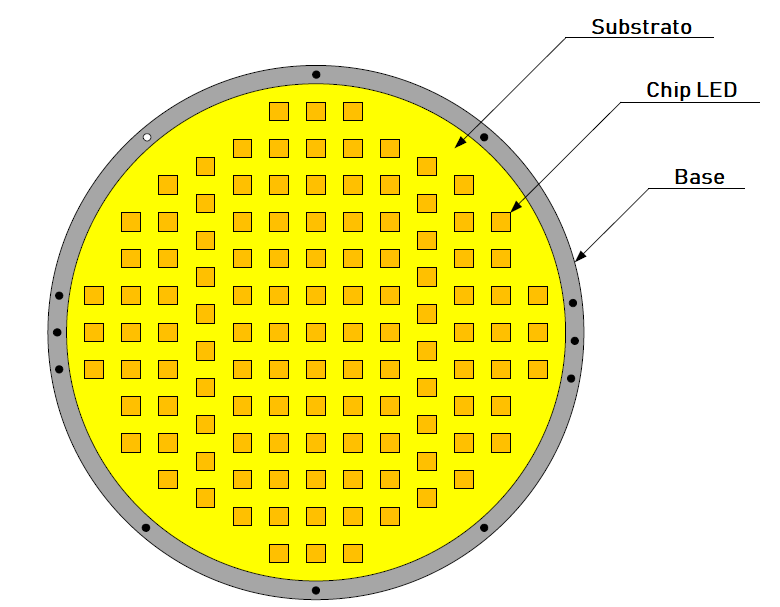
\includegraphics[scale=.4]{../FIGURAS/cob.png}\\
	\fonte{Acervo Pessoal.}
	\label{cob}
\end{figure}

Os EHC (\textit{Extra-High Current}) COB LEDs são uma nova categoria desses dispositivos, de potência da ordem das centenas de watts e fluxo da ordem das dezenas a centenas de milhares de lumens. Trata-se de uma nova classe, pois para atingir estes níveis de fluxo luminoso, tecnologias de assentamento, montagem e arranjo tiveram de ser desenvolvidas para a extração do calor resultante \cite{denis}. Seu uso se dá em aplicações onde se exija luminárias de alta densidade, como estádios, aeroportos, galpões ou plantas industriais.
% centros de tortura,

Devido ao tipo de montagem empregada, sobre um mesmo substrato, a tensão não pode ser muito elevada, sob pena de romper o isolamento dos materiais que compõe o substrato do LED. De fato, estes dispositivos, apesar de processarem altíssima potência, não são encontrados com tensões muito elevadas, geralmente da ordem das dezenas de volts e consequentemente com correntes da ordem das dezenas de amperes, o que dificulta um projeto de acionador, pois este precisa lidar com tal corrente mantendo boa eficiência e baixa transferência de \textit{ripple}.

%Entrar em detalhes sobre física do estado sólido está fora do escopo desta intro 

\section{\textit{Drivers} de acionamento de cargas de iluminação}

Como mencionado na primeira seção, o \textit{driver} é essencial para obtenção de alta eficiência e boa qualidade de iluminação de um dispositivo LED. A seguir, serão explicitados os requisitos geralmente necessários a este elemento.

%tal qual seus primos menos brilhantes
O requisito primário do \textit{driver} é a regulação de corrente. Um LED, assim como os diodos de retificação, apresenta uma relação exponencial da corrente versus tensão, o que significa que ao ligar um deles a uma fonte de tensão, uma variação na tensão causará uma variação exponencialmente maior na corrente, potencialmente causando a destruição do dispositivo.

Por outro lado, um resistor possui uma relação linear bem definida entre corrente e tensão dada pela lei de Ohm. De fato, o acionador de LED mais frequentemente usado em sinalização é o resistor. No entanto, no caso de LEDs de iluminação, de potência significativamente mais elevada, é necessário uma abordagem mais eficiente, para que a tecnologia, ainda de custo elevado, seja competitiva em relação às demais.

Deste modo, os \textit{drivers} em lâmpadas de iluminação LED são quase sempre conversores eletrônicos de potência, devido à eficiência, baixo custo, flexibilidade e tamanho reduzido. Implementações a divisor de tensão reativo ou transformador e retificador também são alternativas, mas têm caído em desuso com o advento de semicondutores cada vez melhores e mais baratos. 

Do lado do dispositivo luminoso, se tem um compromisso com a integridade deste. A tensão nunca deve ser negativa, pois LEDs têm baixa tensão de ruptura e podem entrar em avalanche, sofrendo dano permanente. É comum que um diodo em reverso seja colocado num encapsulamento COB LED para prevenir danos por ESD (\textit{ElectroStatic Discharge}), mas não protegerá de corrente reversa. Cuidado também deve ser tomado com picos espúrios de tensão, frequentemente encontrados em conversores chaveados decorrentes das descontinuidades impostas pelo funcionamento.

A corrente deve ser a variável controlada, e não a tensão, como é comum em fontes reguladas. O conversor deve apresentar vida útil compatível com a do dispositivo luminoso, sabidamente muito elevada, o que requer que certos componentes de vida útil baixa sejam preteridos, sendo o exemplo mais notável os capacitores eletrolíticos \cite{guilherme}. Capacitores de filme metálico, ainda que sejam mais caros e volumosos, são a melhor alternativa para a substituição deles, o que ao mesmo tempo acaba guiando o projeto destes \textit{drivers} num rumo que visa minimizar as capacitâncias presentes. 

Cuidado adicional deve ser tomado com a cintilação, considerando que é custoso para um conversor manter o nível da oscilação do fluxo de potência baixo. A fim de otimizar o projeto, um estudo deve ser feito com o LED a fim de determinar sua resposta em frequência, assim determinando o máximo de oscilação permissível que não seja prejudicial à respectiva finalidade \cite{ieee-flicker}.



%https://youtu.be/tyBmo3i8Eac

\section{Qualidade de energia}

A eficiência não é a única preocupação quando se projeta um dispositivo que irá operar na rede elétrica. Também é importante que seja garantido ao barramento de energia certos critérios, que dizem respeito à qualidade de energia, um ramo especialmente relevante vista a ploriferação das cargas eletrônicas, geralmente não-lineares, na atualidade.

O parâmetro mais facilmente observado é o fator de potência de uma dada carga. Este é definido como a potência real dividida pela potência aparente, equação \ref{fp}, e diz respeito a como a potência está sendo aproveitada, ou seja, se a carga está drenando a menor corrente possível para obter aquele nível de potência.

\begin{equation}
PF_q=\frac{\int_{0}^{T} [V_q(t)\cdot I_q(t)] dt}{V_{q rms} \cdot I_{q rms}}
\label{fp}
\end{equation}

Onde $V_q$ e $I_q$ são tensão e corrente instantânea na carga e $V_{q rms}$ e $I_{q rms}$ seus respectivos valores RMS.

Uma carga de fator de potência unitário em um barramento de corrente alternada senoidal apresentará a corrente igualmente senoidal e em fase com a tensão. Cargas com FP menores irão drenar mais corrente da rede para obter a mesma potência, o que leva a múltiplos inconvenientes, como maiores perdas na linha de transmissão, distúrbios no gerador, desequilíbrio entre fases e outros problemas para a companhia fornecedora de energia \cite{sadiku}.


Uma carga linear apresentará sempre uma corrente de mesmo conteúdo harmônico que sua tensão, ou seja, dada uma entrada senoidal a saída será necessariamente senoidal. Tal conceito não é válido para cargas não-lineares, que são capazes de drenar correntes com formas de onda estranhas à rede, o que é prejudicial. Uma carga em um sistema trifásico cuja corrente contenha terceiras harmônicas, por exemplo, associada com outras do mesmo tipo em fases distintas, irão somar as correntes no neutro, e não se anular, como seria em um sistema equilibrado. Devido a isto, o fio neutro, que nominalmente não deveria conduzir corrente, pode eventualmente ser submetido a uma corrente maior que aquela percorrendo os fios de fase.

Além disso, os equipamentos das linhas de transmissão não são feitos para lidar com correntes harmônicas. Estas introduzem fator de potência nulo, não contribuindo para a potência ativa, levam a problemas de torque espúrio no gerador, reduzindo sua vida útil, podem gerar sobreaquecimento e eventualmente explosão de bancos de capacitores devido a maior corrente RMS nestes, podem causar interferência eletromagnética a equipamentos próximos e poluição do espectro eletromagnético.

A medida para a distorção harmônica de um sinal, chamada de THD (\textit{Total Harmonic Distortion}), é dada pela divisão da intensidade de potência das componentes harmônicas sobre a fundamental, como na equação \ref{thd}.

\begin{equation}
THD_q=\frac{\sqrt{ \sum_{n=2}^{N}A_n^2 }}{A_1}
\label{thd}
\end{equation}

Supondo a tensão perfeitamente senoidal, a THD da corrente é um bom meio de identificar se a carga cumpre satisfatoriamente critérios a respeito de qualidade de energia. O fator de potência pode ser reescrito em termos da THD da seguinte forma:

\begin{equation}
PF_q=\frac{cos(\theta_1)}{\sqrt{ 1+THD^2 } }
\end{equation}

Onde $\theta_1$ é o ângulo de defasagem entre a tensão e a componente fundamental da corrente.


%\section{IEC 61000-3-2}
%\section{IEEE Std 1789 – 2015}

\chapter{Especificação do protótipo}

Neste capítulo é apresentado um panorama geral das topologias de conversores, respectivos modos de operação e sistemas de controle existentes, ponderando suas características e como se adequam ao projeto aqui tratado. Ao fim, serão definidas e justificadas as especificações de funcionamento do protótipo que será desenvolvido no decorrer do trabalho.

Este projeto se refere à construção de um conversor de potência ca-cc off-line, isto é, projetado para ser conectado à rede elétrica ca, acionando um EHC COB LED. Os requisitos funcionais são, portanto, uma potência de saída de 500W a uma tensão entre 40V e 50V e uma tensão de entrada compatível com a fornecida no Brasil, que será adotada senoidal de 60Hz 220V RMS.


\begin{figure}[h]
	\centering
	\caption{Especificações de alto nível requeridas para o \textit{driver}.}
	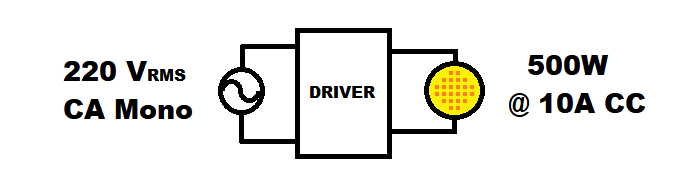
\includegraphics[scale=.8]{../ESQUEMAS/spec.png}\\
	\fonte{Acervo Pessoal.}
\end{figure}

O dispositivo usado será o EHC COB LED Apollo 600, do fabricante FCOpto, que apresenta corrente máxima de 12 A. Os parâmetros elétricos são mostrados na tabela \ref{apollo-spec}, obtidos em \cite{apollo}. Uma extensiva análise experimental do dispositivo foi conduzida em \cite{denis}, de onde foram tomados os parâmetros relativos ao ponto de operação.

\begin{table}[!h]
	\centering
	\caption[Valores máximos dos parâmetros elétricos, térmicos e fotométricos do EHC COB LED Apollo 600.]{%
		\parbox[t]{10cm}{Valores máximos dos parâmetros elétricos, térmicos e fotométricos do EHC COB LED Apollo 600.}}
	\begin{tabular}{|l|l|}
		\hline
		Dissipação máxima de potência     & 608,4 W                                     \\ \hline
		Máxima corrente CC de operação    & 12 A                                        \\ \hline
		Máxima temperatura de junção      & 140$^\circ$ C \\ \hline
		Temperatura de cor correlata      & 5000 K                                      \\ \hline
		Fluxo luminoso na corrente máxima & 60840 lm                                    \\ \hline
	\end{tabular}
	\label{apollo-spec}
\end{table}

O ponto de operação nominal será escolhido em uma corrente média de 10A, de forma a ter certa margem de \textit{ripple} de corrente sem exceder a potência máxima e, potencialmente, destruir o dispositivo.

O \textit{ripple} de baixa frequência da potência de saída e de corrente no EHC COB LED, em 120 Hz, é limitado pela norma de iluminação IEEE PAR 1789 \cite{ieee-flicker}. O fator de potência e a distorção harmônica da corrente de entrada são limitada pela norma IEC 61000-3-2 Classe C \cite{qoe}, de qualidade de energia. Incluem-se ainda, como requisitos, uma eficiência global de conversão de energia superior a 90\% e controlabilidade sobre qualquer distúrbio na tensão de entrada ou saída de até 10\%. Assim estão definidos os requisitos a serem atendidos.

O requisito de fator de potência e distorção harmônica exige um conversor com propriedade PFC, ou \textit{Power Factor Control}, ou seja, deve emular uma carga resistiva para a rede. O controle da corrente na carga é feito por um conversor PC, ou \textit{Power Control}, capaz de regular a corrente de saída suportando variações da entrada ou da carga. Diante disso, três possibilidades se apresentam: usar um conversor de estágio único que cumpra com ambos os requisitos, dois conversores em série, um para correção do fator de potência e outro para PC, ou ainda integrar ambos os estágios num conversor híbrido de alta ordem.

Sobre os modos de operação, existem três alternativas, isto é, DCM (\textit{Discontinuous Conduction Mode}), CCM (\textit{Continuous Conduction Mode}), ou CRM (\textit{CRitical conduction Mode}) \cite{hart}. Os três são exemplificados na figura \ref{ccm_dcm}. No DCM a corrente no indutor sempre cai a zero durante um ciclo de comutação, e no CCM nunca cai a zero em operação normal. No modo crítico o interruptor é ligado imediatamente quando a corrente cai a zero.

\begin{figure}[h]
	\centering
	\caption{Corrente no indutor nos modos de condução descontínua, crítica e contínua, respectivamente}
	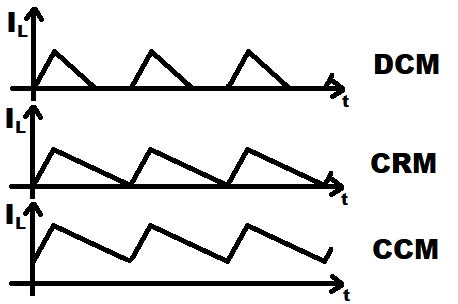
\includegraphics[scale=.8]{../GRAFICOS/dcm_ccm.png}\\
	\fonte{Acervo Pessoal.}
	\label{ccm_dcm}
\end{figure}


Operar em DCM traz alguns benefícios com relação a controlabilidade, pois o conversor passa a possuir função de transferência de ordem um, uma vez que não há memória associada ao indutor, já que este inicia todo ciclo com corrente nula. Esta característica traz, entre outras coisas, maior estabilidade e PFC intrínseco \cite{guilherme-dissert}. No entanto, tal modo de operação deixa de ser atrativo quando a potência a ser processada se torna elevada, uma vez que a corrente tem alto \textit{ripple}, elevando seu valor RMS e consequentemente tendo perdas maiores comparado a um conversor de mesmas especificações de saída operando em CCM. O modo de condução crítica permite um manejamento melhor da corrente com as vantagens do DCM, mas exige que a frequência seja variável, o que confere instabilidade e imprevisibilidade de harmônicas \cite{on}. O CCM, além de apresentar ganho independente do ponto de operação, no caso de empregado no estágio PFC, permite que o filtro EMI seja bastante reduzido ou até eliminado \cite{slua}.

A primeira opção, o conversor de estágio único, é discutida em \cite{guilherme-dissert}. As opções de segunda ordem são os conversores não isolados básicos \textit{buck, boost} e \textit{buck-boost}. Os dois primeiros não permitem muita flexibilidade de tensão de saída, sendo que a do \textit{boost} deve ser maior que a tensão de pico da rede e a do \textit{buck} limitada a um valor baixo, pois enquanto a tensão da rede for inferior à saída não há conversão. Caso projetar a \textit{string} de LEDs estivesse no escopo do projeto, seria possível lidar com isso, porém, como a carga objeto deste trabalho já foi definida, é preciso ter uma saída regulada em torno do ponto de operação estabelecido.

% e a do buck menor que cerca de 100 volts, pois a norma de qualidade de energia impôe um ângulo mínimo de condução, que é tanto menor quanto maior a tensão de saída [tese do pedro]

Podem ser obtidos bons resultados com o \textit{buck-boost}, ou o \'Cuk, já rumando para a quarta ordem, como tratado em \cite{guilherme-dissert}. Porém, devido à alta corrente de saída, os componentes reativos de filtragem exigidos são muito grandes, o que inviabiliza essas topologias para o estudo em questão, onde a corrente envolvida justifica uma abordagem de maior complexidade.

% A topologia de um driver Cùk de estágio único é reproduzida em 

%[seria bom simular um cuk aqui e provar que ele teria um cap absurdo. se der eu faço]

%Tem sido adotada a premissa de se construir conversores o mais compactos possível, por economia de componentes e volume. Diante disso, se dá prioridade ao uso de conversores integrados, os quais condensam [múltiplas células de comutação] em apenas um estágio. Na figura \ref{integrado} temos um exemplo desse tipo de topologia.

%Um conversor integrado condensa [múltiplas células de comutação] em apenas um estágio. Na figura \ref{integrado} temos um exemplo desse tipo de topologia.

A tecnologia de conversores integrados compreende a possibilidade de, em certos casos, combinar as células de comutação de dois conversores distintos em apenas um, simplificando o acionamento. Tal estratégia exige que ambos os conversores sejam projetados para trabalhar na mesma frequência, e o controle de ambos passa a ser dependente um do outro.

Em \cite{bruno} é feito o projeto de um \textit{Buck-Boost Flyback} integrado, cuja topologia é reproduzida na figura \ref{integrado}. O objetivo foi demonstrar a técnica de controle robusto aplicada a um \textit{driver} compacto.

Apesar disso, pesam sobre tal abordagem os altos esforços nos semicondutores, que para o nível de corrente exigido neste estudo seriam impraticáveis, e a baixa eficiência, em torno de 80\% no trabalho citado, devida, em parte pela escolha da topologia, voltada mais à controlabilidade do que eficiência, mas também devido aos tais altos esforços decorrentes da integração.

\begin{figure}[h]
	\centering
	\caption{\textit{Buck-Boost Flyback} integrado.}
	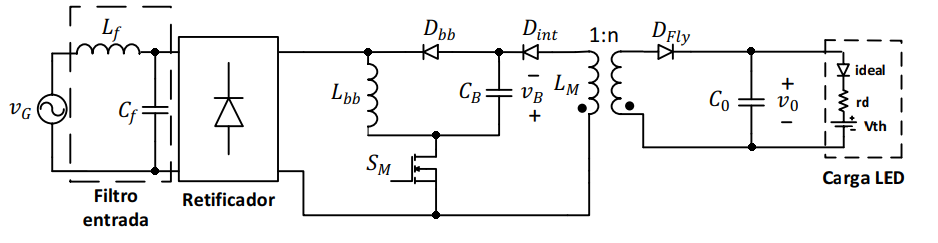
\includegraphics[scale=.5]{../ESQUEMAS/integrado_bruno.png}\\
	\fonte{Acervo Pessoal.}
	\label{integrado}
\end{figure}

Diante disso, pode-se dizer que conversores integrados são alternativas atrativas quando o nível de potência processada é baixo, onde a simplicidade justifica uma perda um pouco mais elevada. Para potências maiores, no entanto, um plano melhor é manter separados os dois estágios, um primeiro capaz de fazer o PFC, e em série, um responsável pelo PC. A figura \ref{two-stage-hl} ilustra a associação de topologias proposta neste trabalho.

%Há também a opção de se utilizar um conversor de dois estágios, que apresenta vantagens com respeito a gerenciamento térmico e eficiência em relação a um integrado, por possuir múltiplas chaves e por ter menos diodos que seus colegas.


%A grande questão 


\begin{figure}[h]
	\centering
	\caption{Circuito esquemático para o acionamento do EHC COB LED em dois estágios, i.e., PFC e PC.}
	\includegraphics[scale=.8]{../ESQUEMAS/twostage.png}\\
	\fonte{Acervo Pessoal.}
	\label{two-stage-hl}
\end{figure}

Para a definição do primeiro estágio, PFC, existem algumas opções a depender das características desejadas. No caso deste trabalho, como explicado na introdução, o principal objetivo é manter a eficiência alta, de modo que descartam-se de imediato topologias isoladas, que não são exigidas no acionamento da carga tratada e notadamente perdem energia no elemento transformador. Por simplicidade, também não é indicada a utilização de conversores de ordem superior, ficando apenas com os de segunda ordem, as topologias \textit{buck, boost e buck-boost}.


O conversor \textit{buck-boost} só deve ser usado em necessidade de se elevar e abaixar a tensão em momentos distintos, pois apresenta baixa eficiência devido a processamento redundante de energia. Assim, surgem duas opções de trabalho, um \textit{buck} ou um \textit{boost}, ou de forma equivalente, escolher uma tensão de barramento acima da tensão de pico ou em um valor baixo. As topologias dos dois conversores mencionados são mostradas na figura \ref{buck_and_boost}.

\begin{figure}[h]
	\centering
	\caption{Conversores \textit{buck} e \textit{boost} como topologias CA-CC}
	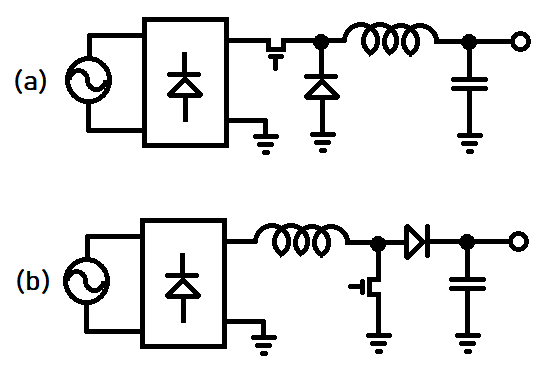
\includegraphics[scale=.8]{../ESQUEMAS/buck_and_boost.png}\\
	\fonte{Acervo Pessoal.}
	\label{buck_and_boost}
\end{figure}

Caso se escolha uma topologia \textit{buck}, a tensão só será abaixada, o que significa que não haverá condução em trechos de cruzamento por zero da senóide da tensão de entrada, de forma que o máximo valor do barramento é fixado pela norma de distorção harmônica, podendo ser calculado em torno dos 130V, caso nenhuma outra forma de distorção seja introduzida \cite{guilherme-dissert}. O ângulo de condução será dado por $4\cdot cos^{-1}(V_o/V_{pk})$, o que significa que para 50V de saída o conversor ficará cerca de 10\% do tempo inativo, desperdiçando parte do tempo de condução dos semicondutores e elevando a capacitância necessária. Já no caso do \textit{boost}, escolhendo uma tensão acima do pico haverá sempre conversão. Além disso, abaixar tensão significa ter que lidar com correntes mais elevadas, o que se traduz em maior perda por condução e ter necessidade de capacitores de barramento maiores, pois a variação da tensão em um capacitor é diretamente proporcional à integral da corrente. O \textit{boost}, por outro lado, apresentará menores correntes e menores capacitores, de forma que é amplamente usado para esse tipo de aplicação e é o que será adotado neste estudo.



%%%%%%%%%%%%%%%%%%%%%%%%%%%%%%%%%%%%%%%%%%%%%%%%%%%%%%%

%, que se sobressai em conversores de média frequência e potência elevada, como o deste trabalho,


%Por ser um conversor on-line, o primeiro estágio deve ser capaz de drenar uma corrente puramente senoidal da fonte, ou o mais perto disso possível. Esse tipo de conversor é dito com PFC, do inglês Power Factor Control. Conversores com operação em DCM possuem PFC intrínseco, ou seja, por não possuírem memória, já que no início de cada ciclo de operação o indutor se encontra descarregado e a tensão de saída é idealmente constante, a corrente segue a tensão de entrada e com um simples filtro EMI se consegue obter corrente de entrada senoidal.


%Os conversores DCM apresentam desvantagens, no entanto. Notavelmente, baixa eficiência e mau uso dos semicondutores. Ambos decorrem do fato de que é necessário garantir a operação em DCM em todos os pontos de operação com a mesma razão cíclica, o que leva a picos de corrente estreitos, e consequentemente dissipação elevada de energia (proporcional ao quadrado da corrente) e necessidade de semicondutores que os suportem, apenas para um curto período. A operação em CCM, por outro lado, permite um aproveitamento muito melhor dos semicondutores.

%Apesar disso, conversores operando em CCM possuem memória, o que pode ser visto em qualquer modelagem como uma ordem a mais. Um conversor que opera em CCM com razão cíclica constante variará muito pouco a corrente de entrada conforme a tensão, tanto menos quanto maior fôr o indutor.

%%%%%%%%%%%%%%%%%%%%%%%%%%%%%%%%%%%%%%%%%%%%%%%


Conversores com operação em DCM possuem PFC intrínseco, ou seja, por não possuírem memória, já que no início de cada ciclo de operação o indutor se encontra descarregado e a tensão de saída é idealmente constante, a corrente segue a tensão de entrada e, com um simples filtro de EMI (\textit{ElectroMagnetic Interference}) se consegue obter corrente de entrada senoidal. Ainda assim, como mencionado anteriormente, existem problemas com baixa eficiência e mau uso dos semicondutores. Ambos decorrem do fato de que é necessário garantir a operação em DCM em todos os pontos de operação com a mesma razão cíclica, o que leva a picos de corrente estreitos, e consequentemente dissipação elevada de energia (proporcional ao quadrado da corrente) e necessidade de semicondutores que os suportem, apenas para um curto período. A operação em CCM, por outro lado, permite um aproveitamento muito melhor dos semicondutores, menores perdas e baixa EMI.

Apesar disso, conversores operando em CCM possuem memória, o que é visto como uma ordem a mais. Um conversor que opera em CCM com razão cíclica constante variará muito pouco a corrente de entrada conforme a tensão, tanto menos quanto maior for o indutor.




Por isso, um \textit{boost} CCM CA-CC deve incluir uma circuitaria a mais, denominada \textit{Active} PFC, para atuar variando a razão cíclica e consequentemente a tensão de entrada de forma a garantir a corrente de entrada senoidal. Desta forma, é conseguido que a corrente de entrada seja modulada como uma senóide sem que caia a zero a cada ciclo de comutação, reduzindo em muito o ruído e permitindo reduzir ou até preterir o filtro EMI.


A tensão de saída deve ser arbitrada de acordo com algumas relações de compromisso. Esta não pode ser muito grande, caso em que as tensões sobre os semicondutores se tornam elevadas e o segundo estágio fica comprometido, pois eventualmente será necessário abaixar a tensão novamente. Ao mesmo tempo, deve ser um pouco superior à tensão de pico para que a razão cíclica não seja pequena demais em alguns momentos. Por fim, uma consideração de ordem prática, quanto maior a tensão menor a corrente e, portanto, menor a capacitância de barramento exigida. No entanto, neste caso, será maior a tensão nominal exigida para os capacitores, os quais são encontrados em tamanhos e tensões discretos. A disponibilidade de tais elementos deve ser levada em conta. Em \cite{slua}, \cite{braga}, é adotada uma tensão de saída de 400V, a qual se adequa bem aos requisitos e será adotada para este projeto.

Em \cite{braga}, é implementado um conversor similar a este, porém utilizando comutação suave. É constatado que se obtém um melhor rendimento utilizando esta técnica, porém, para o caso aqui tratado, a potência processada é cerca de sete vezes menor que naquele estudo, de forma que os poucos watts a serem poupados não justificam a complexidade maior de implementação.


%A boost regulator is an excellent choice for the power stage of an active power factor corrector because the input current is continuous and this produces the lowest level of conducted noise and the best input current waveform. The disadvantage of the boost regulator is the high output voltage required. The output voltage must be greater than the highest expected peak input voltage.



%Segundo estágio abaixando

%extender razão cíclica. Maiores detalhes no capítulo próprio

Tendo definido o primeiro estágio como um \textit{boost} CCM com PFC ativo e $V_{dc}=400V$, deve ser definido o segundo estágio, onde o principal desafio é abaixar a alta tensão do barramento, de 400V, para a tensão nominal do COB LED, que corre em torno dos 40 a 50 volts, dado que o ponto de operação é determinado pela corrente, de até 10A. Obviamente deve ser escolhida uma topologia abaixadora.

Neste estágio, é onde ocorre o processamento das correntes elevadas que caracterizam este estudo, por isso podem ser descartadas as topologias ressonantes, já que as maiores perdas ocorrem justamente por condução, que é o ponto de \textit{trade-off} entre as perdas de comutação minimizadas por estas. Também não é razoável utilizar modos de operação em DCM, por motivos já explicitados.
%que sabidamente aproveitam pouco da capacidade de processamento de potência dos semicondutores e têm perdas mais elevadas por causa dos picos de corrente.

Em um conversor \textit{buck} do tipo convencional, dado na figura \ref{buck}, a razão cíclica, para esta condição será de D=400/50=0.125. Isto é ruim para fins de operação e controle, pois ocorrem elevados picos de corrente durante o período de condução e, como os geradores de PWM (do inglês \textit{Pulse Width Modulation}) no geral trabalham com quantização linear, se perde muito da capacidade de controle, devido ao fato de que cada degrau nesse caso representa uma grande variação percentual sobre o valor nominal da razão cíclica.

\begin{figure}[!h]
	\centering
	\caption{Conversor \textit{Buck} CC-CC}
	\includegraphics[scale=.8]{../ESQUEMAS/_BUCK.PNG}\\
	\fonte{Acervo Pessoal.}
	\label{buck}
\end{figure}

É possível obter um melhor desempenho se utilizando de uma topologia conhecida como IBC, \textit{Interleaved Buck Converter}, que consiste simplesmente de vários conversores \textit{buck} montados em paralelo. Um conversor IBC de duas células é mostrado na figura \ref{ibuck}.


\begin{figure}[!h]
	\centering
	\caption{Topologia de um \textit{Interleaved Buck Converter} com duas células}
	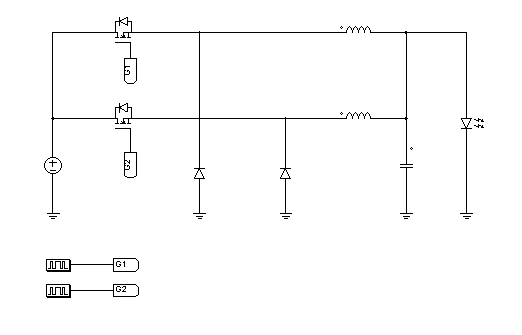
\includegraphics[scale=.8]{../ESQUEMAS/_IBUCK.PNG}\\
	\fonte{Acervo Pessoal.}
	\label{ibuck}
\end{figure}

Nesta topologia, o processamento de energia é dividido entre as duas células, reduzindo à metade a corrente em cada uma, o que, em relação ao \textit{buck} convencional, permite reduzir na metade a frequência de operação, facilitando a construção dos indutores, que precisam de menos fios entrelaçados em paralelo por suportarem uma bitola maior e requerem menor precaução com perdas no núcleo e EMI.

A razão cíclica, no entanto, ainda fica necessariamente no valor calculado anteriormente. Portanto, o problema de controlabilidade não é superado.

Diante disso, foi proposto no artigo \cite{artigo_do_china} uma topologia em que tem-se a interessante característica de redução do ganho estático para uma mesma razão cíclica comparado às topologias abaixadoras normais, como será demontrado no capítulo 3. O conversor, representado na figura \ref{china_1}, é nomeado pelos autores de EDSCIBC (\textit{Extended Duty Cycle Series Capacitor Interleaved Buck Converter}), e é a topologia que será adotada para o segundo estágio.


\begin{figure}[!h]
	\centering
	\caption{Conversor EDSCIBC}
	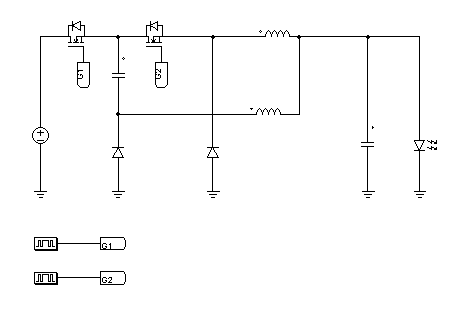
\includegraphics[scale=.8]{../ESQUEMAS/_EDSCIBUCK.PNG}\\
	\fonte{Acervo Pessoal.}
	\label{china_1}
\end{figure}

Assim, tem-se definida a arquitetura a ser implementada. Nos próximos dois capítulos será feito o projeto dos conversores aqui especificados.



\chapter{Análise e projeto do primeiro estágio}

Como discutido no capítulo 1, a melhor opção para o primeiro estágio é um \textit{boost} CCM com PFC ativo. A topologia de um \textit{boost off-line} típico é dada abaixo.

\begin{figure}[h]
	\centering
	\caption{Conversor \textit{Boost} CA-CC}
	\includegraphics[scale=.8]{../ESQUEMAS/boost.png}\\
	\fonte{Acervo Pessoal.}
\end{figure}

Tendo este fator definido, precisa-se agora determinar os valores dos componentes passivos, além de definir a estratégia de controle e seus parâmetros. O capítulo segue com o projeto do circuito de potência e termina com uma simulação para validar o projeto feito.

% e capacidade mínima dos ativos

\section{Estudo de operação}

Como já dito, diferentemente dos conversores CC-CC, um conversor CCM PFC alimentado pela rede CA tem a importante missão de continuamente alterar seu ponto de operação de acordo com a tensão da rede elétrica, de forma a emular uma carga puramente resistiva. Para isso, a corrente no indutor deverá ser como na figura \ref{cmc_wav}. A frequência de comutação foi bastante reduzida para uma representação generalista.

\begin{figure}[!h]
	\centering
	\caption{Corrente no indutor (preto) em um conversor com PF CMC (\textit{Power Factor Current Mode Control}) durante meio ciclo da rede.}
	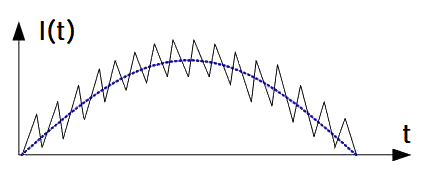
\includegraphics[scale=1]{../RABISCOS/cmc_wav.png}\\
	\fonte{Acervo Pessoal.}
	\label{cmc_wav}
\end{figure}

Pode ser observado que o princípio do balanço volt-segundo não é válido neste caso, pois a corrente média por ciclo de comutação varia conforme a tensão de entrada. De fato, a primeira varia à mesma taxa que a segunda. Assumindo um período de comutação muito pequeno com relação ao período de ciclo da rede, pode-se portanto dizer que o balanço de corrente em um ciclo de comutação será proporcional à derivada da tensão de entrada, $\dot{V}_i(t)$, multiplicada pelo período de comutação. A constante de proporcionalidade será a razão de amplitude entre a corrente e a tensão, ou, substituindo a potência de saída, duas vezes esta sobre o quadrado da amplitude de tensão. Equacionando:

\begin{equation}
\frac{1}{L}V_i(t)D(t)T+\frac{1}{L}(V_i(t)-V_o)(1-D(t))T = \frac{P}{V^2}\dot{V}_i(t)
\label{balance_cmc}
\end{equation}

Onde $V_i$ é a tensão de entrada e $V_o$ a de saída. Isolando D:

\begin{equation}
D(t)=\frac{ \frac{LP}{V_{i_{rms}}^2} \dot{V}_i(t)-V_i(t)+V_o}{V_o}=1+\frac{ \frac{LP}{V_{i_{rms}}^2} \dot{V}_i(t)-V_i(t)}{V_o}
\end{equation}

Finalmente, substituindo a forma de onda senoidal da rede, chega-se na expressão de D.

\begin{equation}
D(t)=\frac{L\cdot P\cdot \omega / V_{s_{rms}}^2 cos(\omega t)-\sqrt{2}V_{s_{rms}}sin(\omega t)+V_o}{V_o}
\label{duty_equation}
\end{equation}

%O ganho estático de um conversor boost é facilmente calculado como:

%\begin{equation}
%G{boost}=\frac{V_o}{V_s}=\frac{1}{1-D}
%\end{equation}

%Para o conversor ser visto como uma carga resistiva, a corrente de entrada deverá ser senoidal e estar em fase com a tensão.

%Assumindo que a dinâmica do conversor é muito mais rápida que a variação de tensão que a ele será imposta, e tomando a variação na tensão de barramento como desprezível, temos:

%\begin{equation}
%\frac{V_o}{V_s(t)}=\frac{1}{1-D(t)}
%\end{equation}

%Isolando D:

%\begin{equation}
%D(t)=1-\frac{V_s(t)}{V_o}
%\end{equation}

Arbitrando um indutor relativamente elevado, de 90mH, de forma a tornar evidente a distorção de \textit{crossover}, e tomando os parâmetros de projeto deste trabalho, a excursão de D durante um semiciclo da rede será como na figura \ref{duty_cmc}.

\begin{figure}[!h]
	\centering
	\caption{Razão cíclica durante um semiciclo da rede}
	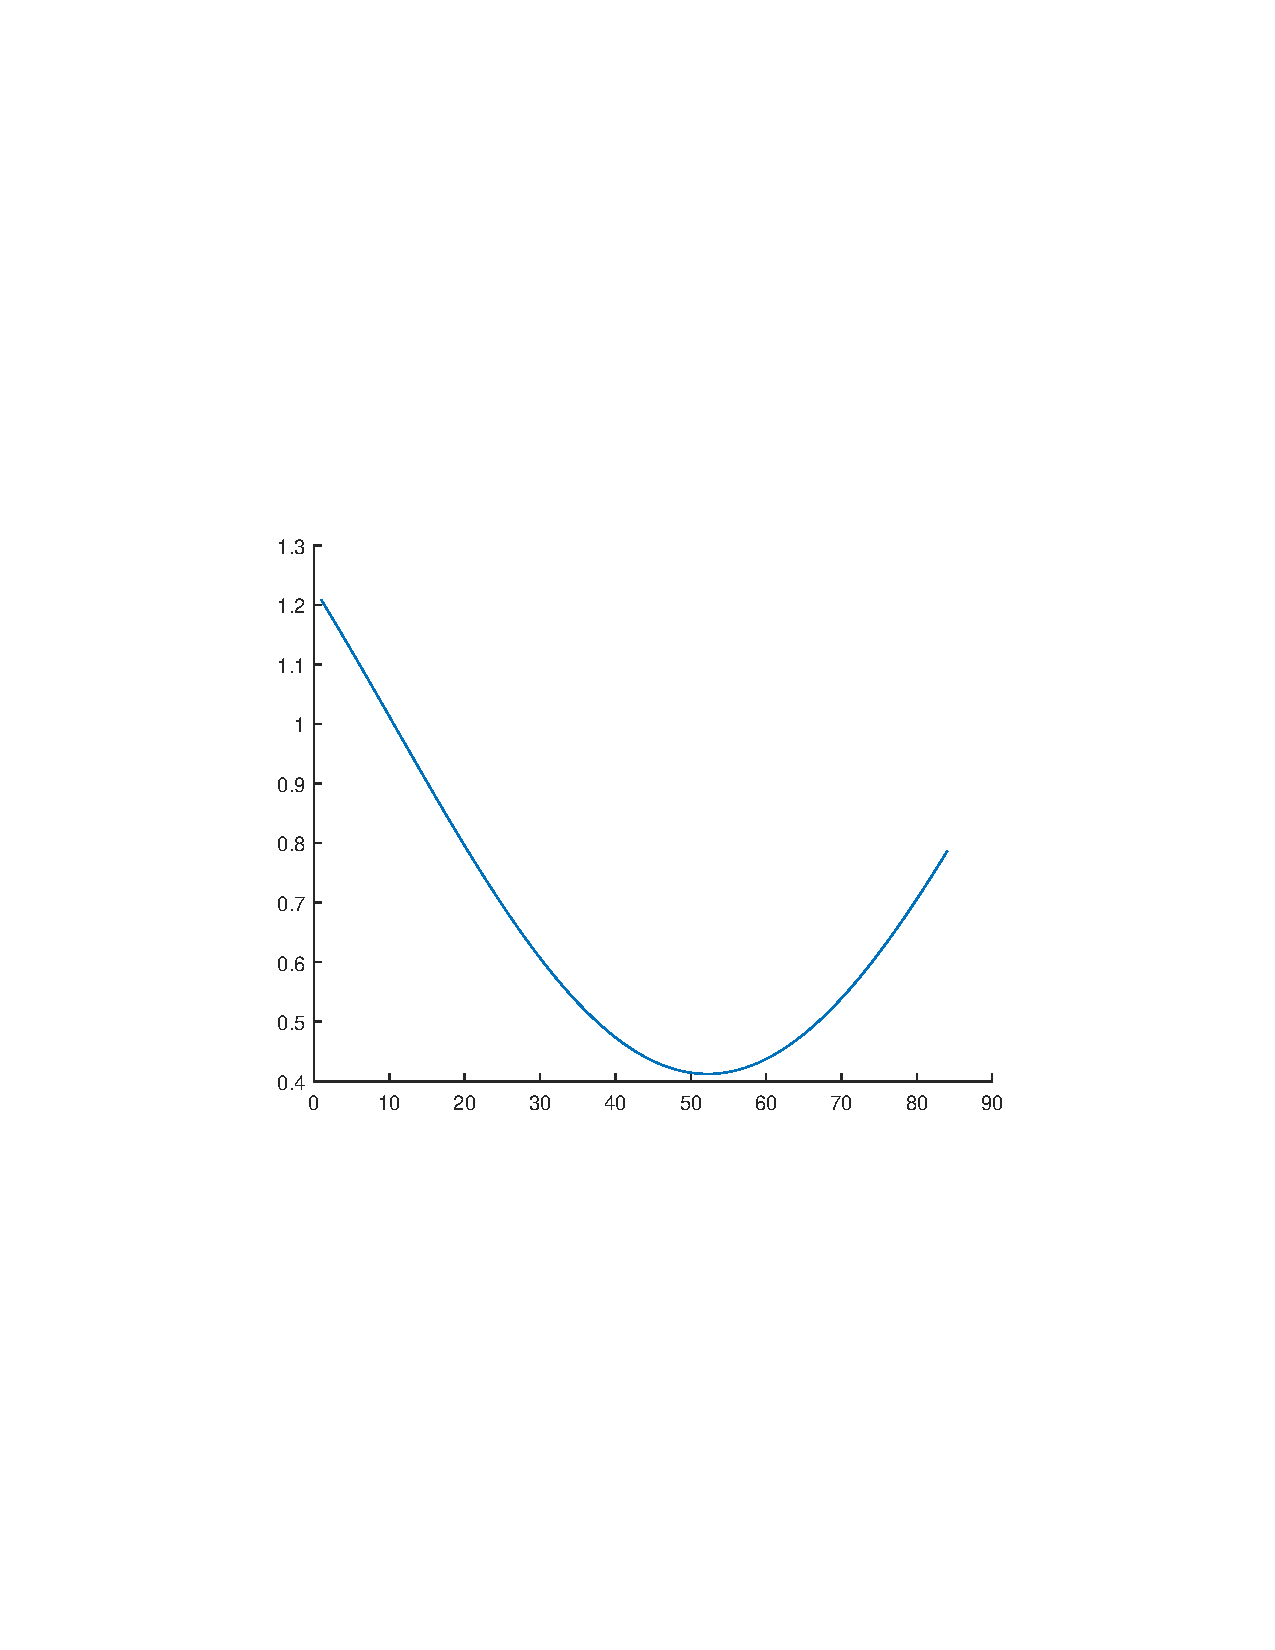
\includegraphics[scale=.6,trim=40mm 70mm 30mm 65mm]{../SCRIPTS/duty.pdf}\\
	\fonte{Acervo Pessoal.}
	\label{duty_cmc}
\end{figure}


%O leitor atento notará 
Pode-se notar que em certo momento é exigida uma razão cíclica maior que a unidade para que a corrente no indutor acompanhe a forma de onda da tensão. Tal proeza é obviamente infactível, destarte esse conversor não é capaz de seguir a forma de onda senoidal imposta. Ainda assim, pode-se mostrar que, ao saturar D, a distorção introduzida é pequena o suficiente para ser ignorada.

Simulando no PSIM\textregistered $\;$ com uma frequência não realista de 1200Hz de modo a evidenciar a comutação, obtêm-se as formas de onda da figura \ref{cmc_waves_psim}. Pode ser notado o momento em que D é saturado e a distorção associada nas correntes do indutor e de entrada.

\begin{figure}[!h]
	\centering
	\caption{\textit{Boost} sujeito à razão cíclica dada em \ref{duty_equation}}
	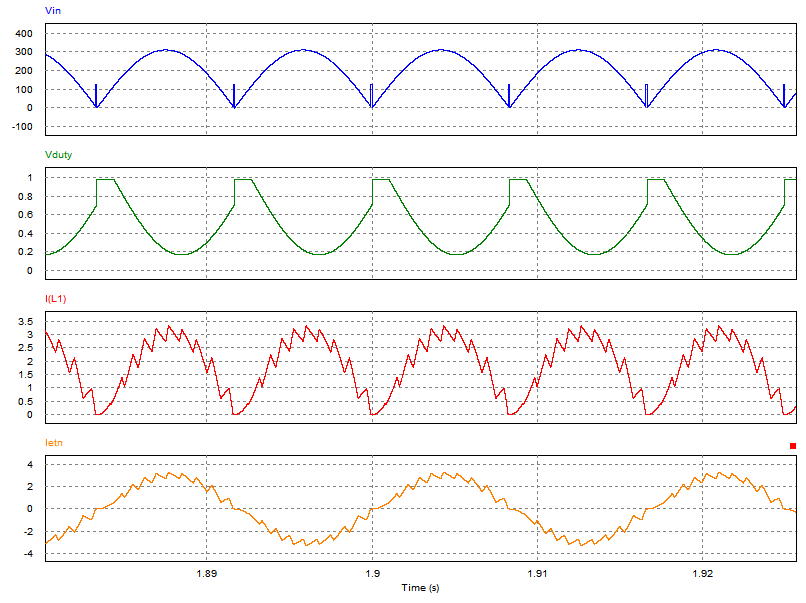
\includegraphics[scale=.5]{../GRAFICOS/PFC_STATIC.png}\\
	\fonte{Acervo Pessoal.}
	\label{cmc_waves_psim}
\end{figure}

Na figura \ref{cmc_waves_psim_2k}, tem-se a forma de onda do indutor em frequência nominal, onde a distorção por comutação praticamente desaparece, deixando evidente a parcela devida à saturação de D. A THD neste modelo foi de 7\% segundo o PSIM\textregistered. Vale notar que há um \textit{trade-off} entre esta distorção e a devido ao \textit{ripple} de alta frequência ao se projetar o valor do indutor.

\begin{figure}[!h]
	\centering
	\caption{Corrente no indutor em um conversor \textit{boost} sujeito à razão cíclica em \ref{duty_equation} com $f_s$ de 60KHz}
	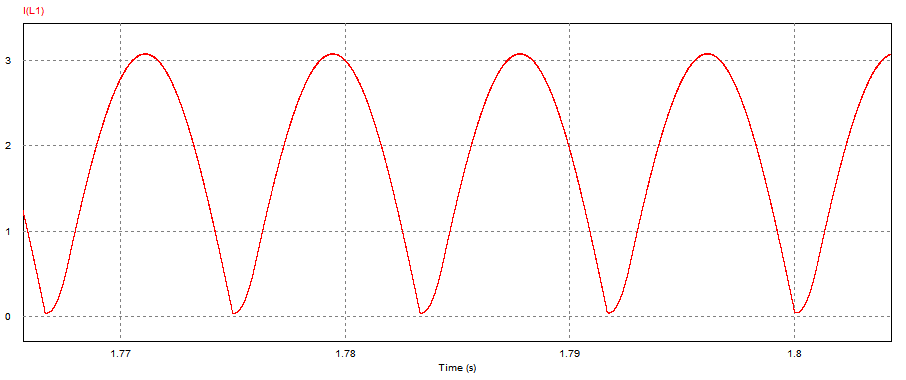
\includegraphics[scale=.4]{../GRAFICOS/PFC_STATIC_20K.png}\\
	\fonte{Acervo Pessoal.}
	\label{cmc_waves_psim_2k}
\end{figure}

O \textit{ripple} de alta frequência pode ser obtido ponderando os intervalos crescente e decrescente de corrente descritos na equação \ref{balance_cmc}. Para este ensaio, o \textit{ripple} terá o perfil mostrado na figura \ref{pfc_ripple}. Vale notar que esta curva pode ser severamente distinta para outro conjunto de especificações. Está além do escopo deste trabalho determinar uma expressão geral para o \textit{ripple} máximo, de forma que o valor no pico da tensão de rede será adotado como uma boa aproximação.

\begin{figure}[!h]
	\centering
	\caption{Intensidade do \textit{ripple} de corrente de alta frequência em um semiciclo da rede}
	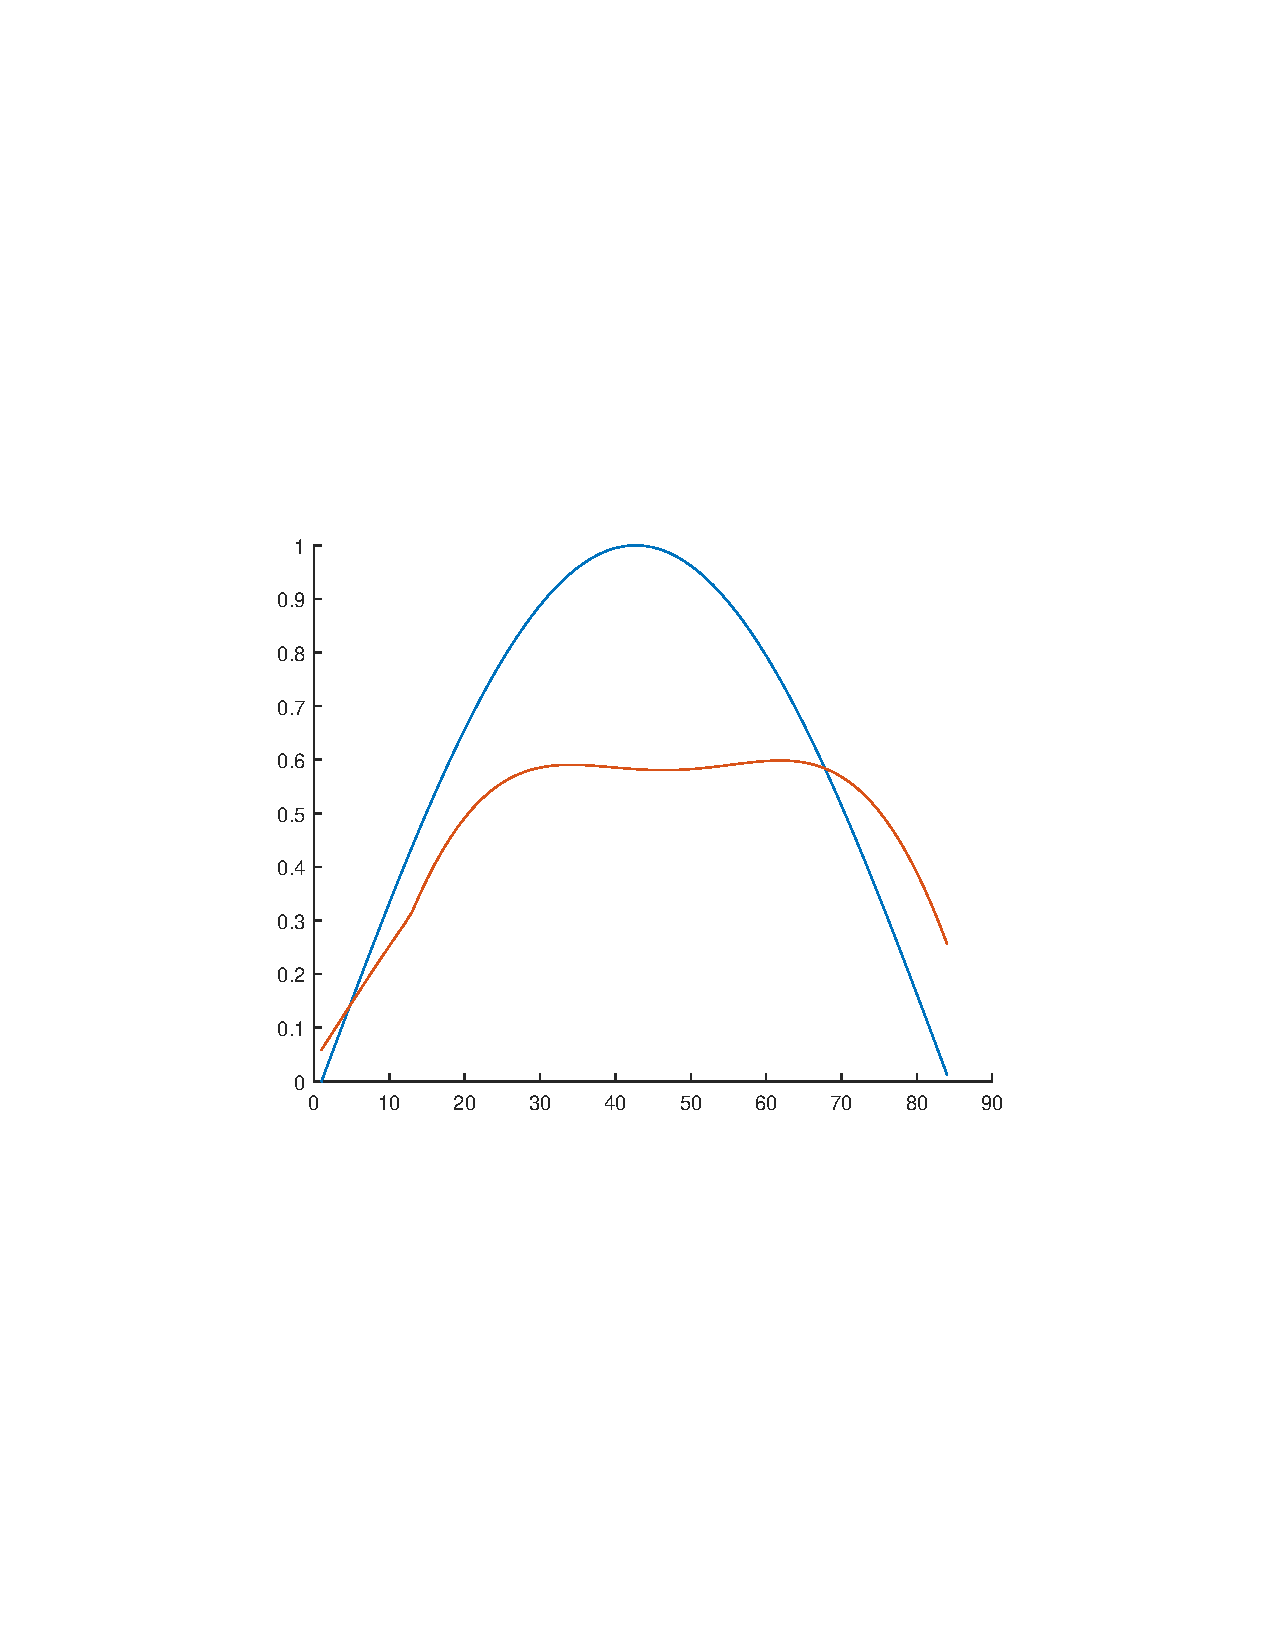
\includegraphics[scale=.6,trim=40mm 70mm 30mm 65mm]{../SCRIPTS/pfc_ripple_2.pdf}\\
	\fonte{Acervo Pessoal.}
	\label{pfc_ripple}
\end{figure}

%Com esse estudo podem ser tiradas como conclusões que o conversor fatalmente flerta com a operação em DCM, mas por pouco tempo, que a corrente de entrada nunca será senoidal, mas chega bem perto, que a corrente máxima do indutor e de entrada é a corrente de pico mais metade da ondulação de corrente, que o \textit{ripple} de alta frequência varia, mas não muito. Com isso podemos seguir rumo à seleção de componentes.

Com esse estudo, podem ser tiradas como conclusões que o conversor fatalmente opera em DCM, mas por um curto intervalo de tempo, durante os cruzamentos por zero da senóide de entrada. Também constatou-se que a corrente de entrada nunca será senoidal, mas é próxima o suficiente. A corrente máxima do indutor e de entrada será a corrente de pico mais metade da ondulação de alta frequência da corrente, e o \textit{ripple} de alta frequência varia conforme o valor instantâneo da tensão da rede CA, mas não de forma significativa. Assim, pode-se seguir rumo à seleção de componentes.


\section{Projeto  dos elementos}

%O projeto de potência aqui transcrito foi primeiro feito em [tcc do Bruno], onde pode ser consultado para maiores explicações.

%O projeto de potência segue como referência a Application Note "UC3854 Controlled Power Factor Correction Circuit Design" \cite{slua}.
Os parâmetros operacionais do conversor são dados na tabela \ref{pfc-spec}.

\begin{table}[!h]
	\centering
	\caption[Parâmetros de projeto para o conversor boost PFC.
	]{
	\parbox[t]{10cm}{Parâmetros de projeto para o conversor boost PFC.}}
	\begin{tabular}{|l|l|}
		\hline
		Tensão de entrada nominal ($V_s$) & 220V  \\ \hline
		Tensão de barramento ($V_b$)      & 400V  \\ \hline
		Potência nominal (P)             & 500W  \\ \hline
		Frequência de operação ($f_s$)    & 60kHz \\ \hline
	\end{tabular}
	\label{pfc-spec}
\end{table}

A tensão de entrada é fornecida pela rede, sendo adotada como 220V RMS. A potência de saída, aproximadamente a de entrada, deve ser de 500W RMS, o que irá drenar uma corrente de entrada aproximadamente senoidal e em fase com a tensão com valor RMS de (500/220)$\approx$2,3 A. Adiante, será discutido como é feito o controle para ser obtida esta corrente. Por ora, assume-se apenas que ele é realizável.





O valor do indutor determina o quanto de \textit{ripple} de alta frequência a corrente de entrada terá, sendo portanto responsável pelo nível de harmônicas de alta frequência que serão introduzidas na rede. Será arbitrado um \textit{ripple} de corrente de 1,5mA.



Como estabelecido na seção anterior, o \textit{ripple} no ponto de pico da tensão da rede CA pode ser adotado como máximo. Ao indicado anteriormente, este é calculado como segue.

\begin{equation}
D_{V_pk}\approx D(\pi / 2\omega) = 1-\frac{\sqrt{2}V_{s_{rms}}}{V_o}
\end{equation}

O \textit{ripple} de corrente será o produto de D pelo tempo de comutação, dividido pelo valor da indutância. Isolando a indutância:

\begin{equation}
L=\frac{D}{\Delta I \cdot f_s}=\frac{1}{\Delta I \cdot f_s}\left (  1-\frac{\sqrt{2}V_{s_{rms}}}{V_o}\right )
\end{equation}

Logo, o indutor deve valer:

% O ponto delimitador é a corrente máxima tolerável, que será a corrente máxima do modelo médio, no pico da tensão senoidal de entrada, somada ao \textit{ripple} de corrente do indutor, ou seja: %deve ser escolhida de 

\begin{equation}
L = \frac{1}{1,5mA \cdot 60kHz}\left (  1-\frac{311V}{400V}\right ) \approx 2,5 mH
\end{equation}

%Assim, admitindo uma corrente de pico máxima de WWA, o indutor deverá ser de ao menos:

O capacitor de saída serve a múltiplos fins, dentre eles filtragem de \textit{ripple} de comutação, da componente de segunda harmônica e estabilidade do conversor, deixando sua banda de passagem menor. Para o caso específico deste estudo, o mais crítico é atenuar o \textit{ripple} de segunda harmônica, e dado que o \textit{ripple} em um capacitor é proporcional à integral da corrente, o barramento de alta tensão é o local ideal para se fazer tal correção, onde se tem a maior tensão e, por conseguinte, a menor corrente na topologia.

A variação de corrente tolerável no COB LED deste estudo é, segundo \cite{denis}, em torno de 25\% da corrente nominal. A resistência dinâmica é próxima de $1\Omega$, logo a variação de tensão aceitável será de 2,5V. O ganho estático de um conversor também é válido para o fator de transferência de \textit{ripple} se a frequência deste for significativamente menor que a de corte do conversor, como de fato exigiremos no projeto de controle do segundo estágio, adiante. Portanto, o \textit{ripple} máximo no barramento intermediário deve ser de $G_m \cdot \Delta V_{cob} = 20V$.

A energia armazenada no capacitor de barramento é igual à integral do balanço de potência neste componente, ou seje:

\begin{equation}
E_C=\frac{CV_b(t)^2}{2}=\int (P_i-P_o)dt
\end{equation}

A potência de entrada é senoidal quadrática, já a de saída é equivalente a que seria dissipada por um resistor, pois o controlador adotado no segundo estágio terá largura de banda inferior à frequência da rede retificada. Sendo $P_m$ a potência média, R a resistência equivalente do segundo estágio, e tomando a derivada dos dois lados:

\begin{equation}
\frac{d}{dt}\left ( \frac{CV_b(t)^2}{2}\right )=CV_b\frac{dV_b}{dt}=2P_msin^2(\omega t)-\frac{V_b^2}{R}
\end{equation}


%A afirmação a seguir parecerá completamente absurda da primeira vez que for lida, mas é fácil perceber que está correta.
A variação da tensão de barramento é desprezível para o cálculo da variação da tensão de barramento. Isto se deve ao fato de que a influência desta variação é uma pequena oscilação da potência de saída, enquanto sua causa primária é a oscilação na potência de entrada. Desta forma podemos tratar $V_b$ como constante, isolar sua derivada e integrar de ambos os lados, isolando a capacitância após isso. Com alguma álgebra, chega-se na seguinte expressão para a capacitância:

\begin{equation}
C = \frac{P}{\omega V \Delta V} \approx \frac{500W}{2\pi \cdot 60 rad/s \cdot 400V \cdot 20V} \approx 160 \mu F
\end{equation}


Termina-se, assim, com os componentes da tabela \ref{gfdp}:

\begin{table}[!h]
	\centering
		\caption[Componentes para o conversor boost PFC.
	]{
		\parbox[t]{10cm}{Componentes para o conversor boost PFC.}}
	\begin{tabular}{|l|l|}
		\hline
		Indutor   & 2,5mH      \\ \hline
		Capacitor & 160$\mu$ F \\ \hline
	\end{tabular}
	\label{gfdp}
\end{table}

\section{Projeto do sistema de controle}

Uma vez determinados os componentes, pode-se projetar o sistema de controle com PFC ativo que irá garantir que a corrente de entrada será senoidal e em fase com a tensão.

Foi tratado matematicamente, no início deste capítulo, o que o sistema de controle deve fazer para que a corrente de entrada tenha o maior fator de potência possível. Aqui será mostrado como fazê-lo.

Existem diversos métodos, alguns deles discutidos em \cite{otro-bruno}. Para este dispositivo, será adotada a estratégia de controle de modo corrente média devido à excelentes características de estabilidade e baixa distorção, pelo fato de amostrar tanto a corrente como a tensão e funcionar numa frequência fixa. Uma forma de onda representativa da corrente do indutor durante meio ciclo foi mostrada na figura \ref{cmc_wav}. Nota-se que a corrente média é senoidal e em fase com a tensão. 



O sistema CMC, \textit{Current Mode Control}, é demonstrado na figura \ref{cmc}, onde se tem a carga, o conversor \textit{boost} e a fonte CA. A tensão de entrada é retificada e filtrada para se obter um valor médio, elevada ao quadrado, devido ao fato de que o fluxo de potência, dada uma impedância fixa, é proporcional ao quadrado da corrente, e passa ao bloco seguinte.

\begin{figure}[!h]
	\centering
	\caption{Conversor \textit{boost} CA-CC com malha de realimentação com controle por corrente média.}
	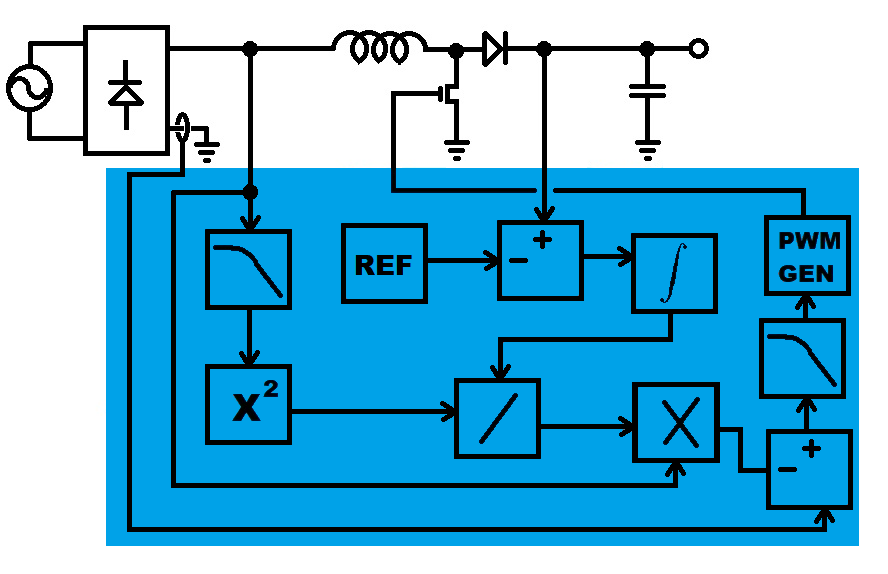
\includegraphics[scale=.4]{../ESQUEMAS/PFC_CTRL.png}\\
	\fonte{Acervo Pessoal.}
	\label{cmc}
\end{figure}


Adiante, a tensão de saída é amostrada e filtrada numa frequência de corte inferior a $2 \cdot 60Hz$, caso contrário esta forçaria o conversor a compensar o \textit{ripple} que naturalmente existe devido ao fluxo de potência ser pulsante e o fator de potência seria prejudicado. O sinal resultante é dividido pelo valor médio da tensão de entrada, para manter o ganho do \textit{loop} de tensão imune à variação na tensão de entrada, e multiplicado pela forma de onda desta para obter a senóide retificada que garantirá fator de potência unitário. Finalmente, este sinal é somado à leitura da corrente passada por um compensador tipo 2 e comparada à onda triangular para obter o sinal de comutação para o MOSFET (\textit{Metal-Oxide Semiconductor Field Effect Transistor}).
%passado por uma malha de controle proporcional-integral e esta leitura é

Os parâmetros a serem calculados são a frequência de corte do filtro da tensão de entrada, que deve ser feito ponderando resposta à variação na tensão de entrada e estabilidade, e os parâmetros do integrador, sobre o qual também pesam questões de estabilidade, mas ainda a resposta a variações na saída do conversor.


Para a implementação do controle descrito, será usado o tradicional CI UC3854 \cite{uc3854}, da unitrode, uma fabricante atualmente pertencente à Texas Instruments. O diagrama interno do circuito integrado é reproduzido na figura \ref{uc}.

\begin{figure}[!h]
	\centering
	\caption{Circuitaria interna do CI UC3854}
	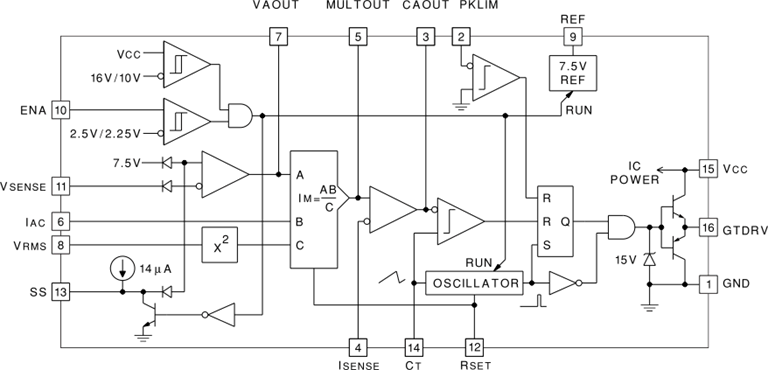
\includegraphics[scale=.7]{../RABISCOS/fbd_slus336a.png}\\
	\fonte{Datasheet do CI UC3854 \cite{uc3854}.}
	\label{uc}
\end{figure}

Nesta figura, além dos elementos citados anteriormente, nota-se alguns mais necessários ao funcionamento e outros opcionais. Tem-se um oscilador a circuito RC ressonante, pelo qual escolhe-se a frequência de operação, comparadores que desligam o \textit{driver} para serem usados como proteção a sobrecorrente e sobretensão, um circuito de \textit{soft-starter} e obviamente terminais de alimentação e capacitores para estabilização da referência interna. O projeto segue como referência a Application Note "UC3854 Controlled Power Factor Correction Circuit Design" \cite{slua}, disponibilizada pela Unitrode, cujo diagrama recomendado é reproduzido na figura \ref{slua}. As equações de projeto foram retiradas do mesmo documento.

\begin{figure}[!h]
	\centering
	\caption{Circuito recomendado pela Unitrode}
	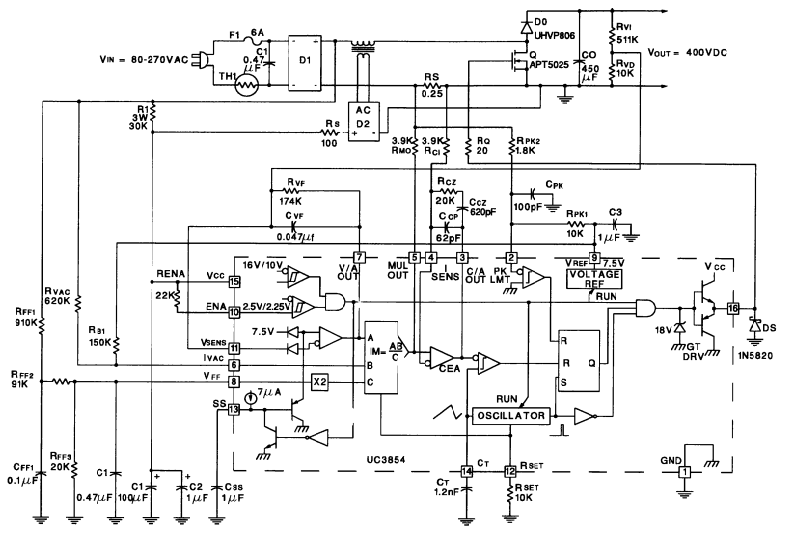
\includegraphics[scale=.7]{../RABISCOS/SLUA.png}\\
	\fonte{Aplication Note SLUA144 \cite{slua}.}
	\label{slua}
\end{figure}

Na entrada $V_{FF}$, ou tensão de \textit{FeedFoward}, deve ser fornecido o valor médio da tensão de entrada, para isso será usado simples filtro de segunda ordem como o da figura \ref{vff}. A tensão deve estar entre 1,4V e 4,5V. Acima disso a tensão lida será grampeada e o conversor perderá o controle \textit{feedfoward}, abaixo o multiplicador irá saturar e a corrente será totalmente distorcida, portanto é melhor que o conversor opere mais próximo do limite superior. Além disso, é recomendado que a tensão do segundo nó não caia abaixo dos 7,5V. Se arbitrada uma tensão mínima de entrada de 80V, os resistores podem ser obtidos resolvendo as equações que seguem.

\begin{figure}[!h]
	\centering
	\caption{Filtro de segunda ordem da entrada de controle \textit{feedfoward}}
	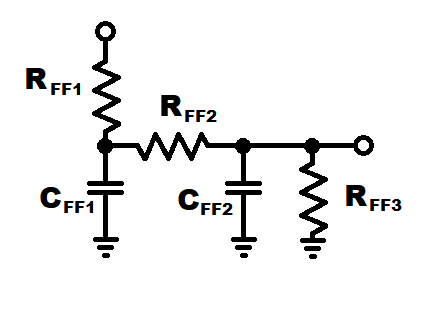
\includegraphics[scale=.7]{../ESQUEMAS/vff.png}\\
	\fonte{Acervo Pessoal.}
	\label{vff}
\end{figure}

\begin{equation}
\begin{cases}
R_{ff1}+R_{ff2} =\left( \frac{V_{min}\cdot 0,9}{1,4} -1 \right) \cdot R_{ff3}\\
R_{ff2} =\frac{7,5 \left( R_{ff1}+R_{ff2}+R_{ff3}\right)}{0,9V_{min}} \cdot R_{ff3}
\end{cases}
\end{equation}

Arbitrando-se $Rff3=10k\Omega$, os valores restantes serão $Rff2=39k\Omega$ e $Rff1=470k\Omega$. Os dois capacitores devem ser escolhidos de modo que a frequência de corte da rede seja baixa o suficiente para não prejudicar o fator de potência, mas ainda alta para que o controle seja efetivo. Colocam-se os dois pólos em uma frequência de um décimo da rede, ou 6Hz. Se a interferência da primeira rede RC na segunda for desprezada e a impedância de entrada do CI suposta infinita, os capacitores serão simplesmente:

\begin{equation}
C_{ff1}=\frac{1}{(R_{ff2}+R_{ff3})S}\approx 620nF
\end{equation}

\begin{equation}
C_{ff2}=\frac{1}{R_{ff3}S}\approx 2,5 \mu F
\end{equation}


O segundo filtro é o compensador responsável por manter a saída com erro nulo em estado permanente. Este deve ser portanto um integrador, como mostrado na figura \ref{vfo}.

\begin{figure}[!h]
	\centering
	\caption{Compensador da tensão de saída}
	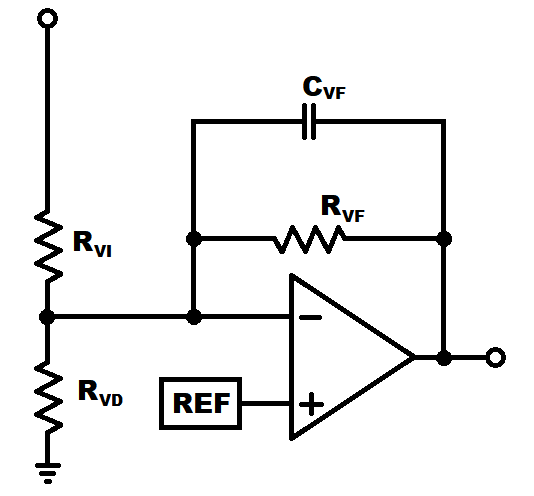
\includegraphics[scale=.5]{../ESQUEMAS/vfo.png}\\
	\fonte{Acervo Pessoal.}
	\label{vfo}
\end{figure}

A referência é interna ao chip, de 7,5V. Para os resistores $R_{vi}$ e $R_{vd}$, portanto, basta percorrer uma lista de resistores comerciais e escolher os que melhor se aproximam desta tensão para uma entrada de 400V, altos o suficiente para não dissipar muita potência. Seleciona-se $R_{vi}=470k\Omega$ e $R_{vd}=9k\Omega$.

Os componentes do integrador devem ser calculados fechando a malha de controle e resolvendo em função da THD máxima aceitável. Para o caso tratado, admitindo 1,5\% de distorção, serão obtidos os seguintes:

\begin{equation}
R_{vf}=\frac{F_r}{F_{vi}}R_{vi}G_{va}\approx 180k \Omega
\end{equation}

\begin{equation}
C_{vf}=\frac{1}{2\pi F_r R_{vi}G_{va}}\approx 620 nF
\end{equation}

Por fim, a corrente deve ser amostrada para poder ser controlada. Isto é feito com um resistor na linha de retorno da corrente, onde convenciona-se terra. O resistor sensor, $R_s$, é arbitrado de forma a não haver perda desnecessária de potência mas ainda assim ter um valor de tensão apreciável para leitura. Será usado uma resistência de $0,2\Omega$, conseguida com dois resistores de 2w $0,39\Omega$ em paralelo. A figura \ref{vci} mostra o compensador de corrente.

\begin{figure}[!h]
	\centering
	\caption{Compensador da malha de corrente}
	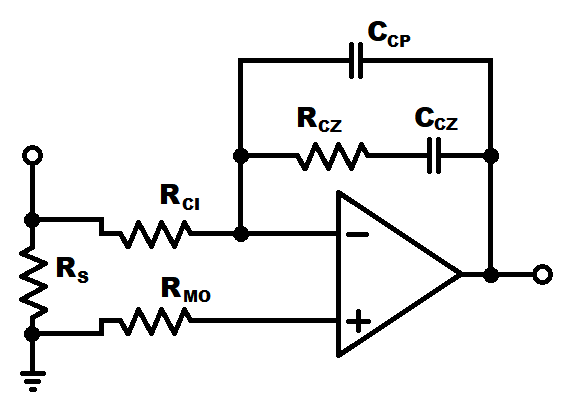
\includegraphics[scale=.5]{../ESQUEMAS/vci.png}\\
	\fonte{Acervo Pessoal.}
	\label{vci}
\end{figure}

%%%%%%%%%%%%%%%%%%%%%%%%%%%%%%%%%%
Os resistores $R_{ci}$ e $R_{mo}$ são arbitrados em 4,7k$\Omega$. O ganho DC do compensador deve ser de tal forma que a inclinação descendente da leitura da corrente no indutor seja igual à da onda triangular gerada pelo oscilador, de amplitude 5,2V, ou seja:

\begin{equation}
\Delta V_{R_s}=\frac{V_o}{L}\frac{R_s}{F_s}
\end{equation}

\begin{equation}
G_{ca}=\frac{5,2}{\Delta V_{R_s}}
\end{equation}

\begin{equation}
R_{cz}=R_{ci}G_{ca}
\end{equation}

O resistor $R_{cz}$ assim calculado vale aproximadamente $39k\Omega$. O pólo do compensador deve ser colocado a uma década abaixo da frequência de comutação, então $C_{cp}$ se calcula como segue.

\begin{equation}
C_{cp}=\frac{1}{2\pi f_s R_{cz}}
\end{equation}

O capacitor obtido assim vale 48pF. O zero deve ser alocado numa frequência intermediária, dada por:

\begin{equation}
f_{ci}=\frac{f_s}{G_{ca}}\frac{R_{cz}}{2\pi R_{ci}}
\end{equation}

\begin{equation}
C_{cz}=\frac{1}{2\pi f_{ci} R_{cz}}
\end{equation}

E chega-se a um $C_{cz}$ de 330pF.

%%%%%%%%%%%%%%%%%%%%%%%%%%%%%%%%%%

No manual da Unitrode, é fornecido uma metodologia para determinar os demais componentes do sistema de controle. Uma folha de cálculo do \textit{software} CAS Maxima\textregistered ~com as equações pode ser consultada em \cite{github}.
%Além dos parâmetros explicados acima, existem malhas de proteção que devem ser calculadas para desarmar o comutação em caso de falha, sobre as quais não entraremos em detalhes.



%O ci implementa a exata cadeia de controle descrito, e 


%Falo um pouco de como funciona o ci, depois ressuscito aquele projeto

%Aqui os componentes calculados para a implementação.

%:table

\section{Simulação}

O conversor foi simulado usando um modelo do UC3854, nativo do PSIM\textregistered ~ \textit{circuit simulator}. O modelo totalmente implementado é reproduzido na figura \ref{psim_boost}.

\begin{figure}[!h]
	\centering
	\caption{Conversor \textit{boost} com UC3854.}
	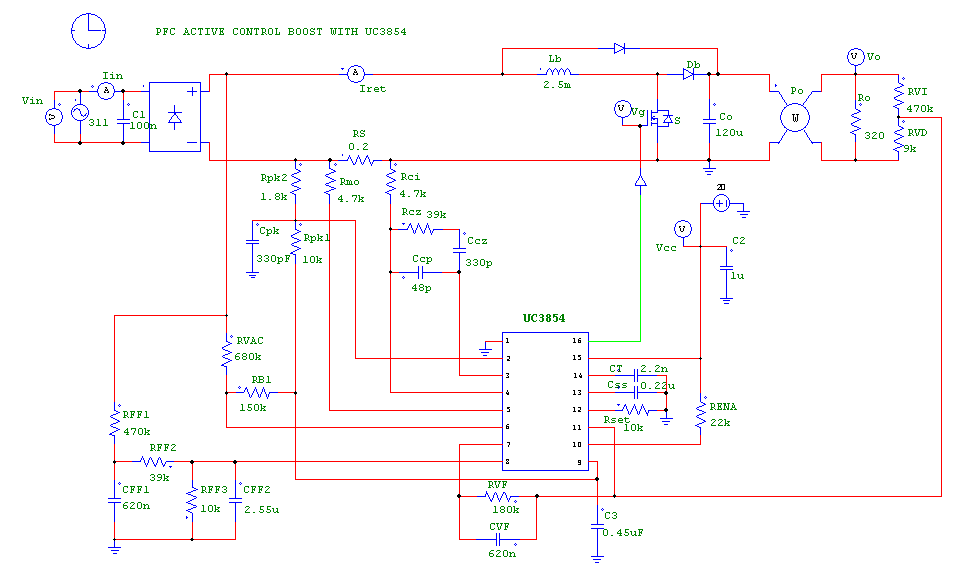
\includegraphics[scale=.6]{../ESQUEMAS/PFC_BOOST.PNG}\\
	\fonte{Acervo Pessoal.}
	\label{psim_boost}
\end{figure}

Na figura \ref{psim_boost}, pode-se ver que a corrente de entrada é bastante próxima de senoidal, graças à corrente modulada no indutor. A tensão de saída apresenta o \textit{ripple} de baixa frequência calculado de 20V e a potência de saída é próxima aos 500W, como especificado.

\begin{figure}[!h]
	\centering
	\caption{Corrente de entrada, tensão de saída, potência de saída e corrente no indutor em um \textit{boost} com UC3854.}
	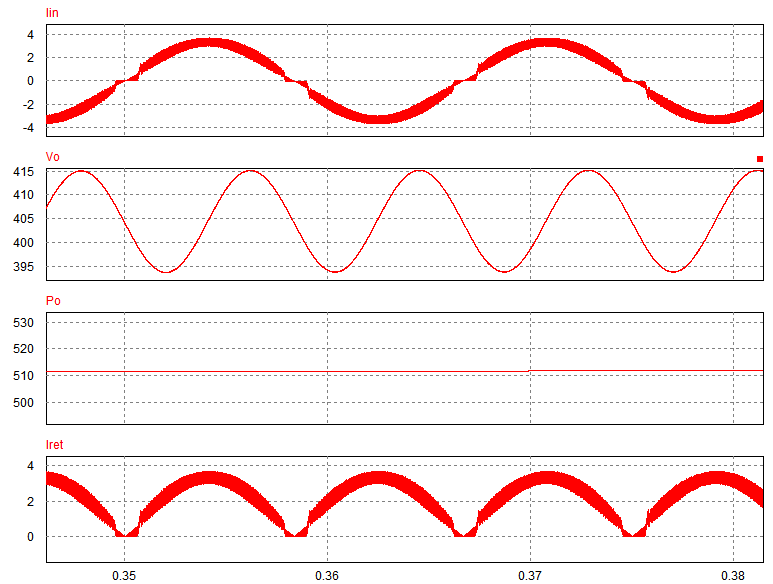
\includegraphics[scale=.5]{../GRAFICOS/pfc_output.PNG}\\
	\fonte{Acervo Pessoal.}
	\label{pfc_output}
\end{figure}

Por fim, na figura \ref{pfc_pertub}, o conversor é sujeito a uma variação de 10\% na tensão de entrada. Pode-se ver que a saída volta ao estado estacionário em poucos ciclos de rede, o que, para todos os efeitos, atente bem a aplicação à qual é destinado.

\begin{figure}[!t]%!h
	\centering
	\caption{Corrente de entrada, tensão de saída, potência de saída e corrente no indutor em um \textit{boost} com UC3854 sujeito a distúrbio na entrada.}
	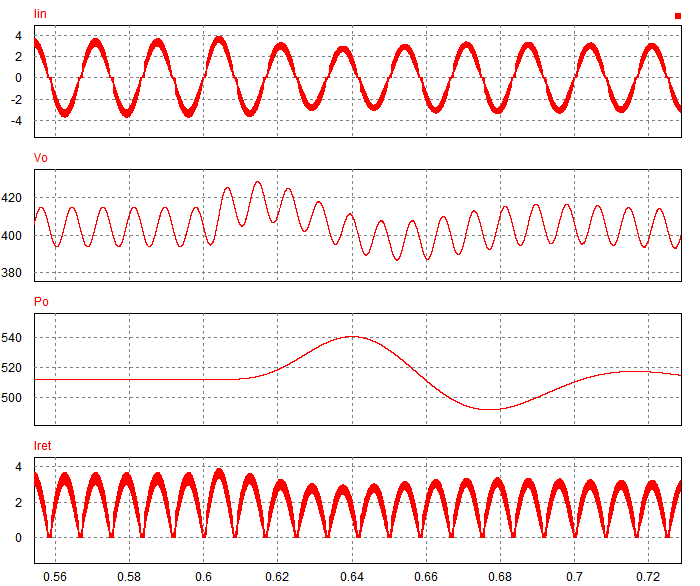
\includegraphics[scale=.6]{../GRAFICOS/pfc_pertub.PNG}\\
	\fonte{Acervo Pessoal.}
	\label{pfc_pertub}
\end{figure}

\chapter{Análise e projeto do segundo estágio}

Como definido anteriormente, a topologia do segundo estágio será aquela tratada em \cite{artigo_do_china}, reproduzida na figura \ref{china}. Adiante, será caracterizada a operação do conversor e definidos os parâmetros de implementação.

\begin{figure}[!h]
	\centering
	\caption{Conversor EDSCIBC}
	\includegraphics[scale=.8]{../ESQUEMAS/EDSCIBUCK.PNG}\\
	\fonte{Acervo Pessoal.}
	\label{china}
\end{figure}


\section{Estudo de operação}

O conversor EDSCIBC, quando operando em CCM, possui dois comportamentos distintos, um para uma razão cíclica inferior a 0,5, quando não ocorre condução simultânea dos interruptores, e outro, para maior que meio, quando isto ocorre. É notável que a aplicação deste trabalho excursiona longe do segundo comportamento, portanto apenas o primeiro será analizado.

\begin{figure}[!h]
	\centering
	\caption{Etapas da operação do conversor EDSCIBC: (a) primeira etapa, (b) terceira etapa, e (c) segunda e quarta etapas.}
	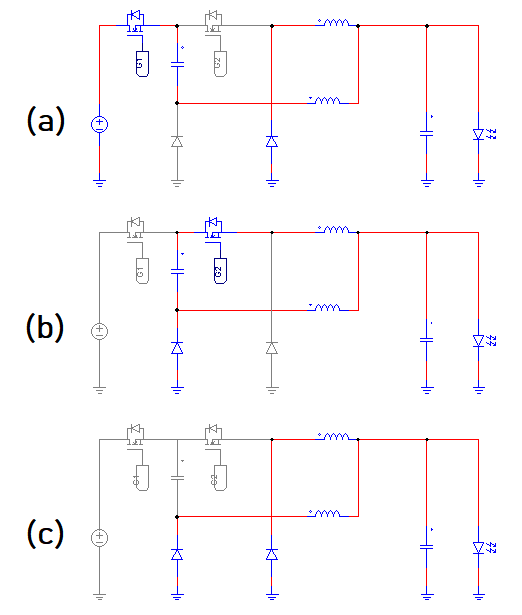
\includegraphics[scale=.8]{../ESQUEMAS/split.PNG}\\
	\fonte{Acervo Pessoal.}
	\label{modos}
\end{figure}

É tomado como estágio inicial de operação o fechamento do interruptor S1. Neste período de duração $T \cdot D$ o interruptor S2 e o diodo D1 se encontram abertos, como visto na figura \ref{modos} (a). Será obtido o modelo em espaço de estados do conversor. Para isso, tomam-se as variáveis de estado como as assocoadas à energia armazenada, as correntes nos indutores e tensões nos capacitores, como mostrado na figura \ref{ss_var}. Desta forma, chega-se ao seguinte:


\begin{figure}[!h]
	\centering
	\caption{Variáveis de estado definidas sobre o EDSCIBC}
	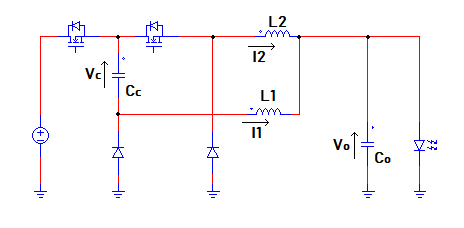
\includegraphics[scale=.8]{../ESQUEMAS/ss_var.PNG}\\
	\fonte{Acervo Pessoal.}
	\label{ss_var}
\end{figure}

% As tensões nos indutores, assumindo \textit{ripple} nulo nos capacitores de acoplamento e de saída, serão:


\begin{equation}
\begin{array}{cc}
L_1 \dot{I}_1 = V_s - V_c - V_o\\
L_2 \dot{I}_2 = - V_o\\
C_c \dot{V}_c = I_1\\
C_o \dot{V}_o = I_1+I_2-\frac{V_o}{R_o}
\end{array}
\end{equation}

Ou na forma matricial:

\begin{equation}
\begin{array}{cc}
\begin{bmatrix}\dot{I_1} \\\dot{I_2} \\\dot{V_c} \\\dot{V_o}\end{bmatrix}=\begin{bmatrix}0&0&-1/L_1&-1/L_1 \\ 0&0&0&-1/L_2 \\ 1/C_c&0&0&0 \\ 1/C_o&1/C_o&0&0\end{bmatrix}\begin{bmatrix}I_1 \\I_2 \\V_c \\V_o
\end{bmatrix}+\begin{bmatrix}V_s/L_1 \\0\\0\\-I_o/C_o\end{bmatrix}\\\\
%y(t)=\begin{bmatrix} 0&0&0&1 \end{bmatrix}\begin{bmatrix} I_1 \\I_2 \\V_c \\V_o\end{bmatrix}
\end{array}
\end{equation}



Depois disso ocorre a abertura do interruptor S1, e a parte funcional do conversor se torna como a figura \ref{modos} (c) durante T(1-2D)/2. As equações de estado serão:

\begin{equation}
\begin{array}{cc}
L_1 \dot{I}_1 = - V_o\\
L_2 \dot{I}_2 = - V_o\\
C_c \dot{V}_c = 0\\
C_o \dot{V}_o = I_1+I_2-\frac{V_o}{R_o}
\end{array}
\end{equation}

\begin{equation}
\begin{array}{cc}
\begin{bmatrix}\dot{I_1} \\\dot{I_2} \\\dot{V_c} \\\dot{V_o}\end{bmatrix}=\begin{bmatrix}0&0&0&-1/L_1 \\ 0&0&0&-1/L_2 \\ 0&0&0&0 \\ 1/C_o&1/C_o&0&0\end{bmatrix}\begin{bmatrix}I_1 \\I_2 \\V_c \\V_o
\end{bmatrix}+\begin{bmatrix}0\\0\\0\\-I_o/C_o\end{bmatrix}\\\\
%y(t)=\begin{bmatrix} 0&0&0&1 \end{bmatrix}\begin{bmatrix} I_1 \\I_2 \\V_c \\V_o\end{bmatrix}
\end{array}
\end{equation}

No terceiro estado, de duração $T \cdot D$, o interruptor S2 e o diodo D1 conduzem, como na Figura \ref{modos} (b). As equações de estado serão expressas por:

\begin{equation}
\begin{array}{cc}
L_1 \dot{I}_1 = - V_o\\
L_2 \dot{I}_2 = V_c - V_{o}\\
C_c \dot{V}_c = -I_2\\
C_o \dot{V}_o = I_1+I_2-\frac{V_o}{R_o}
\end{array}
\end{equation}

\begin{equation}
\begin{array}{cc}
\begin{bmatrix}\dot{I_1} \\\dot{I_2} \\\dot{V_c} \\\dot{V_o}\end{bmatrix}=\begin{bmatrix}0&0&0&-1/L_1 \\ 0&0&1/L_2&-1/L_2 \\ 0&-1/C_c&0&0 \\ 1/C_o&1/C_o&0&0\end{bmatrix}\begin{bmatrix}I_1 \\I_2 \\V_c \\V_o
\end{bmatrix}+\begin{bmatrix}0\\0\\0\\-I_o/C_o\end{bmatrix}\\\\
%y(t)=\begin{bmatrix} 0&0&0&1 \end{bmatrix}\begin{bmatrix} I_1 \\I_2 \\V_c \\V_o\end{bmatrix}
\end{array}
\end{equation}

Por último, o quarto estado é idêntico ao segundo, apresentado na figura \ref{modos} (c), e com a mesma duração. Assim, pode-se encontrar o modelo médio do conversor, ponderando as equações de estados pelo tempo de duração relativo de cada um \cite{ogata}.

\begin{equation}
\begin{array}{cc}
\begin{bmatrix}\dot{I_1} \\\dot{I_2} \\\dot{V_c} \\\dot{V_o}\end{bmatrix}=\begin{bmatrix}0&0&-D/L_1&-1/L_1 \\ 0&0&D/L_2&-1/L_2 \\ D/C_c&-D/C_c&0&0 \\ 1/C_o&1/C_o&0&0\end{bmatrix}\begin{bmatrix}I_1 \\I_2 \\V_c \\V_o
\end{bmatrix}+\begin{bmatrix}DV_i/L_1\\0\\0\\-I_o/C_o\end{bmatrix}\\\\
y(t)=\begin{bmatrix} 0&0&0&1 \end{bmatrix}\begin{bmatrix} I_1 \\I_2 \\V_c \\V_o\end{bmatrix}
\end{array}
\end{equation}

% Usando o princípio do balanço volt-segundo, podemos igualar a variação positiva e negativa nas correntes dos indutores, obtendo as equações abaixo.

%\begin{equation}
%%\left
%\{
%\begin{array}{lll}
%\frac{1}{L1} (V_{s} - V_{cb} - V_{o}) \cdot DT = \frac{1}{L1} V_{o}(1-D)T\\
%\frac{1}{L2} (V_{cb} - V_{o}) \cdot DT = \frac{1}{L2} V_{o}(1-D)T
%\end{array}
%%\right%\}
%\label{system_ind}
%\end{equation}
%
%Somando as duas e isolando $ V_{o} / V_{s} $, chegamos que o ganho estático vale:


Em estado estacionário, $\dot{X}=0$. Logo:

\begin{equation}
\begin{array}{lll}
0=AX+U\\
X=-A^{-1}U
\end{array}
\end{equation}

Resolvendo e isolando $V_o$, chega-se, finalmente, a:

\begin{equation}
G_{e} = \frac{V_{o}}{V_{s}} = \frac{D}{2}
\end{equation}


Portanto, metade do ganho geralmente obtido em conversores \textit{buck} ou IBC convencionais, o que significa que será operado a uma razão cíclica nominal duas vezes maior.

Um dos efeitos adversos é uma corrente de valor bastante alto passando pelo capacitor de acoplamento, que precisa ser dimensionado para tal, com respeito à dissipação térmica e perdas por ESR (\textit{Equivalent Series Resistance}). Outro problema, este de ordem mais prática, é que o capacitor, mesmo em série com os indutores, acaba sofrendo um pouco com as variações bruscas de tensão decorrentes da comutação, levando a alguns picos consideráveis de corrente, como pode ser observado nas imagens de osciloscópio do capítulo referente ao ensaio do protótipo.

\section{Projeto dos elementos}

%Para garantir o modo de operação em ccm, os indutores deverão ter um valor mínimo, como calculado a seguir. Começamos por encontrar a corrente média em cada um deles:

A corrente média nos indutores é determinada pela carga. Como observado nas equações \ref{system_ind}, derivadas isolando as indutâncias das equações de estados, os dois indutores são sujeitos às mesmas tensões. Além disso, pode-se constatar na figura \ref{modos} que não ocorre fluxo de corrente de um indutor para o outro em nenhuma das quatro etapas de funcionamento. Portanto, escolhendo valores de indutância iguais, as correntes em ambos serão idealmente idênticas, defasadas de $180^\circ$ e de valor médio igual à metade do valor médio da corrente de saída.

\begin{equation}
\begin{cases}
\frac{1}{L1} (V_{s} - V_{cb} - V_{o}) \cdot DT = \frac{1}{L1} V_{o}(1-D)T\\
\frac{1}{L2} (V_{cb} - V_{o}) \cdot DT = \frac{1}{L2} V_{o}(1-D)T
\end{cases}
\label{system_ind}
\end{equation}

Desta forma, toma-se como figura de mérito a máxima variação da corrente instantânea no indutor sobre a corrente média deste, $\Delta I_L/I_L$. Usando as equações em \ref{system_ind}, esta grandeza será a dada em \ref{variation}.

\begin{equation}
\frac{\Delta I_L}{I_L} = \frac{\frac{1}{L} \cdot V_{o}(1-D)T}{I_{L_{media}}} = 
\frac{ V_{o}(1-D)}{LI_{L_{media}}F}
\label{variation}
\end{equation}

Isolando L:

\begin{equation}
L = \frac{V_{o}(1-D)}{\Delta I_L \cdot f_s}
\end{equation}

A variação de corrente é simétrica em relação à corrente média, portanto um $\Delta I_L/I_L=2$ retornaria a indutância crítica, que valeria:

\begin{equation}
L_{crit} \approx \frac{ 50V(1-0,25)}{2 \cdot 5A \cdot 40KHz} \approx 100 \mu H
\end{equation}

No entanto, tal indutância colocaria o conversor num limiar de funcionamento instável, onde uma pequena mudança de parâmetros o faria mudar de modo de operação, tal qual uma mudança na corrente de saída ou na tensão de entrada. Além disso, trabalhar com uma excursão elevada de corrente nos obriga a dimensionar núcleos maiores nos indutores, pois a corrente de saturação precisará ser maior, e o laço de histerese será mais extenso, resultando em perda de eficiência. Visando ainda a possibilidade de dimerização, onde a corrente de saída seria eventualmente reduzida, será arbitrado um ${\Delta I_L}/{I_L}$ de 0,4. Os indutores, portanto, deverão ser:

\begin{equation}
L_{ot} \approx \frac{ 50V(1-0,25)}{0,4 \cdot 5A \cdot 40KHz} \approx 450 \mu H
\end{equation}


Os capacitores são obtidos pelo nível de \textit{ripple} aceitável arbitrado para a respectiva função. Para o capacitor de acoplamento, assume-se um \textit{ripple} máximo tolerável de 4\%. Observando os modos de operação, percebe-se que a corrente que flui no capacitor de acoplamento é a mesma que passa nos indutores nos modos (a) e (b) da figura \ref{modos}. Usando um capacitor ideal:
%e, para a saída adota-se segundo normas de iluminação e o estudo em [artigo do denis] um máximo de O

\begin{equation}
V_{C} = V_0 + \frac{1}{C} \int_{0}^{T} i(t) dt =
V_0 + \frac{1}{C} \int_{-DT/2}^{DT/2} (i_m + (V_s/2-V_o)t) dt
\end{equation}

\begin{equation}
\Delta V_C = \frac{1}{C} [i_m \cdot t + (V_s/2-V_o)t^2/2]^{D/2}_{-D/2} = \frac{I_m \cdot D}{C \cdot F}
\end{equation}

Isolando a capacitância e substituindo $N_C = \Delta V / V_{medio}$:

%\begin{equation}
%C = \frac{2 \cdot I_m \cdot D}{\Delta V \cdot F}
%\end{equation}

\begin{equation}
C = \frac{4 \cdot I_m \cdot D}{N_C \cdot V_s \cdot F} \approx 
\frac{4 \cdot 5A \cdot 0,25}{0,04 \cdot 400V \cdot 40KHz} \approx 8 \mu F
\label{cap_ac}
\end{equation}


%\begin{eqnarray*}
%	x &=& blah blah blah \\ 
%	& & more blah blah blah 
%\end{eqnarray*}




Para o capacitor de saída, deve ser considerada a resistência dinâmica do COB LED, que segundo \cite{denis} vale aproximadamente $1 \Omega$ para o ponto de operação almejado. Assim pode-se arbitrar um \textit{ripple} de alta frequência máximo de 100mA, que equivale a um \textit{ripple} de tensão de 100mV. A corrente de saída será a soma das correntes dos dois indutores, que possuem formas de onda triangulares com 180 graus de defasagem de uma para a outra. Encontrar o \textit{ripple} da soma é um exercício simples de geometria analítica, para este conjunto de parâmetros vale cerca de 3/4 do \textit{ripple} de um dos indutores, especificado na definição do próprio, numa frequência duas vezes maior. A área de um triângulo de desvio da média será metade do produto de metade do \textit{ripple} pela metade do período de comutação, e o \textit{ripple} na tensão o dobro disso dividido pela capacitância. Isolando a capacitância:

\begin{equation}
C = \frac{\Delta I_L}{4 \cdot \Delta V_o \cdot F} \approx 
\frac{0,4 \cdot 0,75 \cdot 5A}{4 \cdot 100mV \cdot 80KHz} \approx 40 \mu F
\end{equation}


O primeiro interruptor é sujeito à mesma tensão de entrada, já o segundo fica submetido a apenas metade desta tensão, devido à queda de tensão do capacitor de acoplamento. Um MOSFET possui resistência de condução, logo deve ser especificada para ele a corrente RMS. Já um diodo apresenta queda de tensão aproximadamente constante, e por isso este deve ser especificado em função da corrente média. Restringiu-se bastante a variação na intensidade da corrente dos indutores como especificação de projeto, de forma que pode ser desprezada para os efeitos desse cálculo. A corrente nos interruptores e nos diodos pode ser aproximada como na figura \ref{a_semi}, (a) e (b), respectivamente.

\begin{figure}[!h]
	\centering
	\caption{Correntes nos semicondutores: (a) corrente no MOSFET S1 e (b) corrente no diodo D1.}
	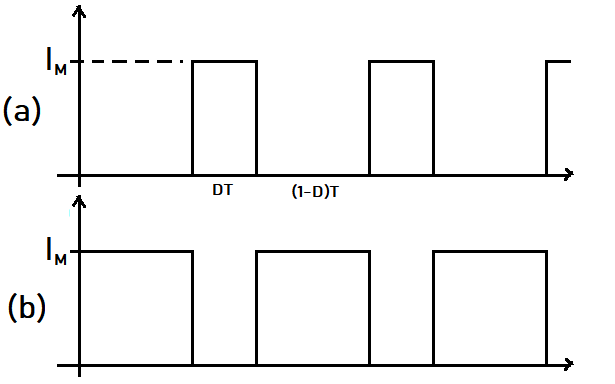
\includegraphics[scale=.4]{../GRAFICOS/a_semi.PNG}\\
	\fonte{Acervo Pessoal.}
	\label{a_semi}
\end{figure}

Assim a corrente RMS será de $I_m \sqrt{D} \approx 2,5A $ para os MOSFETs e a corrente média de $I_m (1-D) \approx 3,8A $ para os diodos. Devem ser escolhidos semicondutores que suportem tais esforços com alguma tolerância. Desta forma são definidos os componentes listados na tabela \ref{comp-pc}.

\begin{table}[!h]
	\centering
\caption[Valores calculados para os componentes do circuito de potência do conversor do estágio PC.]{
	\parbox[t]{10cm}{Valores calculados para os componentes do circuito de potência do conversor do estágio PC.}}
	\begin{tabular}{|l|l|}
		\hline
		Indutores                & $450\mu H$ \\ \hline
		Capacitor de acoplamento & $8 \mu F$  \\ \hline
		Capacitor de saída       & $40 \mu F$ \\ \hline
	\end{tabular}
\label{comp-pc}
\end{table}






\section{Projeto do sistema de controle}

O conversor, como modelado em \cite{denis}, admitindo indutâncias iguais e tensão no capacitor de acoplamento constante, e tomado o modelo do COB LED como uma queda de tensão constante e uma resistência dinâmica medida para o ponto de operação nominal, terá a seguinte função-transferência \cite{denis}:

\begin{equation}
H(s)=\frac{V_o(s)}{D}=\frac{V_{dc}/r_d}{(C_oL)s^2+(L/r_d)s+2}
\end{equation}

Será utilizado um controlador do tipo integrador, cuja equação no domínio contínuo é a seguinte:

\begin{equation}
G(s) = \frac{1}{s}
\end{equation}

Como critérios para o projeto do controlador, priorizando a estabilidade, tomam-se:

\begin{itemize}
	\item Margem de fase de ao menos 60 graus.
	\item Tempo de acomodação de 5 ciclos da rede.
	\item Frequência de corte inferior a 20\% de $2 \cdot 60Hz$
\end{itemize}

Foi constatado que uma constante de integração de A=4,3e-4 $mA^{-1}$ é capaz de cumprir tais requisitos. Discretizando a função transferência pelo método trapezoidal, obtém-se a seguinte função no domínio discreto:

\begin{equation}
G(z) = \frac{Y(z)}{X(z)} = \frac{A(z+1)}{z-1}
\end{equation}

Isolando em Y, chega-se à seguinte lei de controle:

\begin{equation}
Y[N] = Y[N-1] - A(X[N] + X[N-1])
\end{equation}

O controle é implementado de forma digital, utilizando para isso um sensor de corrente e um processador equipado com gerador de PWM. Uma interrupção programada síncrona com o gerador PWM desencadeia uma leitura da corrente, que é usada para alimentar a equação de controle, a qual fornece um novo valor de razão cíclica, que por sua vez é usada para atualizar a largura do sinal de controle das chaves.
% A estrutura do controle segue o fluxo descrito na figura \ref{controle_digital}.

Fazer a amostragem síncrona com o PWM traz algumas vantagens. A começar pela resposta do controle, que é a mais rápida possível para a mesma margem de estabilidade, já que o valor da razão cíclica é atualizado a cada ciclo de comutação, e não há maneira de atualizar mais rapidamente.

Outra vantagem é que o sistema fica menos suscetível a ruídos de comutação, pois as frequências de ordem superior são significativamente filtradas pelo capacitor de saída e, como a amostra é tomada sempre no mesmo lugar com relação ao ciclo de operação do conversor, a frequência de comutação e harmônicas são mapeadas por efeito de \textit{aliasing} na frequência zero, ou CC, não contribuindo com oscilação no controle.


%Projeto do controle (Modelagem consulte Denis), estabilidade, discretização, considerações sobre aliasing (tenho uma teoria boa pra essa parte kkkk) e tá bão já.

\section{Simulação}

Tendo definido os componentes e parâmetros operacionais, foi testado em simulação no \textit{software} PSIM o funcionamento do conversor. O modelo da figura \ref{pc_model} foi utilizado.

\begin{figure}[h]
	\centering
	\caption{Conversor EDSCIBC no PSIM}
	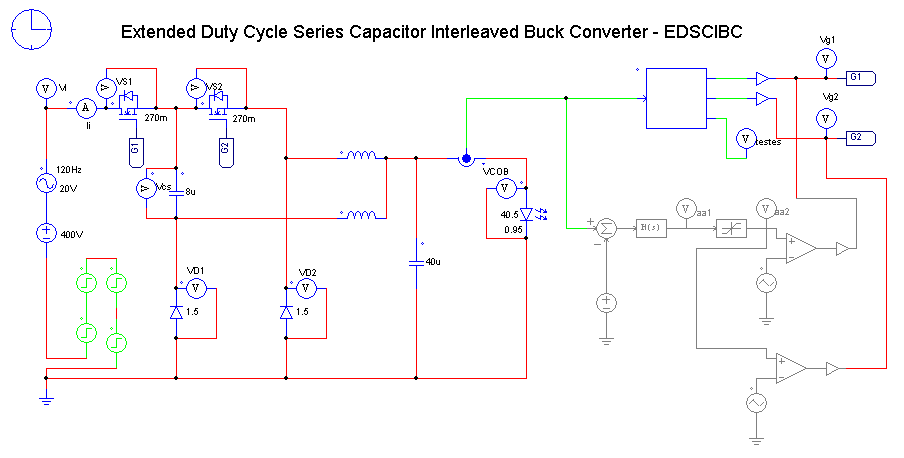
\includegraphics[scale=.7]{../ESQUEMAS/Ctrl_egibc_2.PNG}\\
	\fonte{Acervo Pessoal.}
	\label{pc_model}
\end{figure}

Este modelo permite simulação tanto de controle digital como de analógico. Para o caso digital, o seguinte código foi usado dentro da unidade de simulação computacional:


\begin{lstlisting}
PWM_MAX = PWM_PERIOD * D_CRIT;
PWM_MIN = PWM_PERIOD * D_MIN;

// FREQ SIMULATION = 40MHz

ct++;
if(ct>DUTY)*out=0;
if(ct>499 && ct<(499+DUTY))*(out+1)=15;
if(ct>(499+DUTY))*(out+1)=0;
if(ct>998){ct=0;*out=15;ctt++;}

if(ctt>9){
    ctt=0;
    corrente = -*in;     //A*ui32ADC0Value + B;

    x[2]=x[1];
    x[1]=x[0];
    x[0]= REF - corrente;

    //Malha de controle

    ymv[1]=ymv[0];
    ymv[0] = 5.38e-09*(x[0]+ x[1])+ymv[1];

    // Hard - Limiter
    if (ymv[0] > 0.5) {
        ymv[0] = 0.5;
    } else if (ymv[0] < 0) {
        ymv[0] = 0;
    }
    *(out+2)=ymv[0];

    PWM_NEW=ymv[0];

    //Limitador de razao ciclica
    if (PWM_NEW > D_CRIT) {
        PWM_NEW = D_CRIT;
    } else if (PWM_NEW < D_MIN) {
        PWM_NEW = D_MIN;
    }

    //Calculo da razao ciclica
    DUTY = PWM_NEW*PWM_PERIOD;
}
\end{lstlisting}

Trata-se de uma linguagem c simplificada, sem detalhes de implementação física, porém é possível entender a essência do necessário a um controlador digital. A cada período, a corrente é amostrada e as variáveis responsáveis pela memória são atualizadas. Posteriormente, o valor de saída do controle é atualizado de acordo com a equação de diferenças do controlador e uma cascata de saturadores garante que o conversor não opere em um ponto potencialmente destrutivo.

A implementação prática exige algumas minúcias que serão tratadas no capítulo próprio. Nas próximas imagens serão mostradas formas de onda simuladas relevantes ao funcionamento do conversor.

Na figura \ref{stage2_hf} são apresentadas as tensões sobre os interruptores no primeiro \textit{grid}, sobre os diodos no segundo e as correntes nos indutores no terceiro. Como previsto, apenas um dos semicondutores é sujeito à tensão de entrada, vendo os outros apenas a metade desta. As correntes nos indutores são defasadas de $180^\circ$, e apresentam \textit{ripple} de alta frequência de 2A, como projetado.

\begin{figure}[!h]
	\centering
	\caption{Tensões nos interruptores, nos diodos, e correntes nos indutores}
	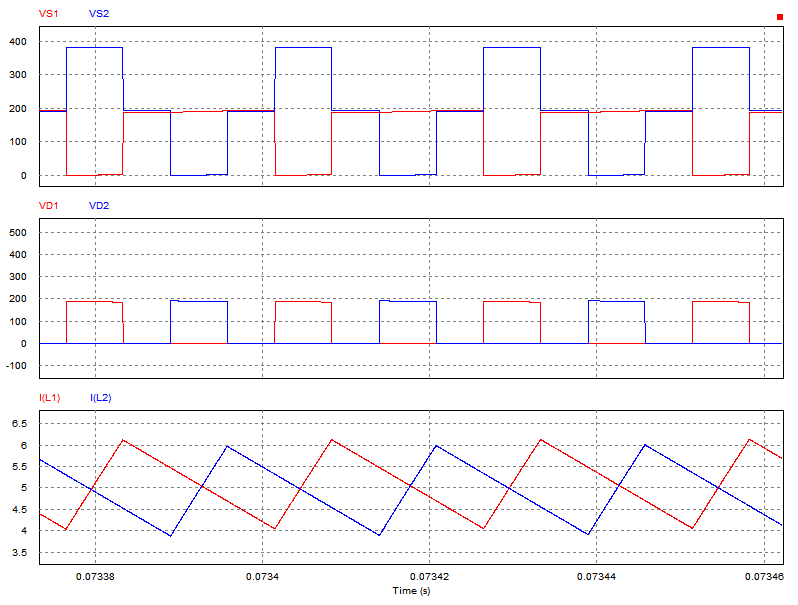
\includegraphics[scale=.5]{../GRAFICOS/stage2_hf.PNG}\\
	\fonte{Acervo Pessoal.}
	\label{stage2_hf}
\end{figure}

O \textit{ripple} de baixa frequência de 20V foi introduzido no barramento, a fim de simular o funcionamento do primeiro estágio. De acordo com a figura \ref{stage2_rip}, o \textit{ripple} se propaga para a saída, com aproximadamente 2,5V de pico a pico, pouco menos que o projetado devido a não ter sido considerada a capacitância de saída do segundo estágio para o projeto do capacitor de barramento. A corrente, de igual forma, apresenta ondulação de baixa frequência de 25\% da média. 

\begin{figure}[!h]
	\centering
	\caption{Tensão e corrente de saída}
	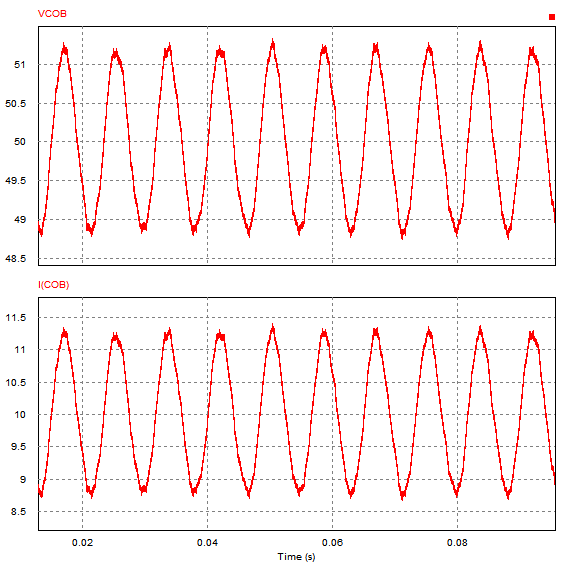
\includegraphics[scale=.7]{../GRAFICOS/stage2_rip.PNG}\\
	\fonte{Acervo Pessoal.}
	\label{stage2_rip}
\end{figure}

Por fim, conforme apresentado na figura \ref{stage2_ctrl}, é feito um ensaio aplicando um distúrbio de 10\% na tensão média de entrada. A potência de saída sofre certa variação, porém rapidamente volta à média, próximo aos 500W.

\begin{figure}[!h]
	\centering
	\caption{Tensão de entrada sujeita a distúrbio, tensão e potência de saída}
%	\includegraphics[scale=.5]{../GRAFICOS/stage2_ctrl.PNG}\\
	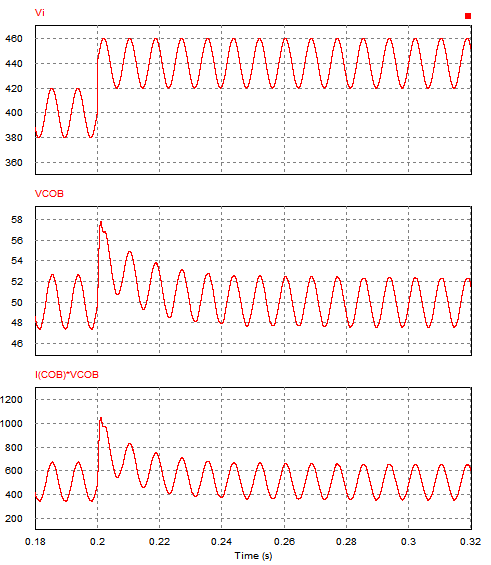
\includegraphics[scale=.75]{../GRAFICOS/pc_disturb.PNG}\\
	\fonte{Acervo Pessoal.}
	\label{stage2_ctrl}
\end{figure}




\chapter{AIT - Assembly, Integration and Test}

Como esboçado nos capítulos anteriores, o conversor é composto de dois estágios. Complementam as placas de potência dispositivos de acionamento, sensores, interfaces e controladores. Neste capítulo, serão descritos os materiais, equipamentos e métodos de construção e ensaio do protótipo, bem como apresentadas as formas de onda obtidas.

\section{Primeiro estágio}

O primeiro estágio foi implementado com base nas notas de aplicação da Unitrode\textregistered ~\cite{slua}. A placa do conversor foi produzida em fenolite face simples no Laboratório de Processos da UFJF e o protótipo montado no NIMO.

O indutor foi fabricado em núcleo E NEE 55-28-21, da THORNTON, com 90 voltas de 3 fios AWG 24 entrelaçados em paralelo. A tabela \ref{pfc-matlist} resume os demais componentes.

\begin{table}[!h]
	\centering
	\caption[Indutor, capacitor e modelos dos semicondutores utilizados no protótipo do conversor boost PFC.]{
		\parbox[t]{10cm}{Indutor, capacitor e modelos dos semicondutores utilizados no protótipo do conversor boost PFC.}}
	\begin{tabular}{|l|l|}
		\hline
		Indutor                 & 2,7 mH    \\ \hline
		Capacitor de barramento & 160 $\mu F$    \\ \hline
		Ponte retificadora      & KBU8K     \\ \hline
		MOSFET                  & IPW60R190 \\ \hline
		Diodo                   & MUR 860   \\ \hline
	\end{tabular}
\label{pfc-matlist}
\end{table}

\begin{figure}[!h]
	\centering
	\caption{Protótipo PFC - Placa de potência}
	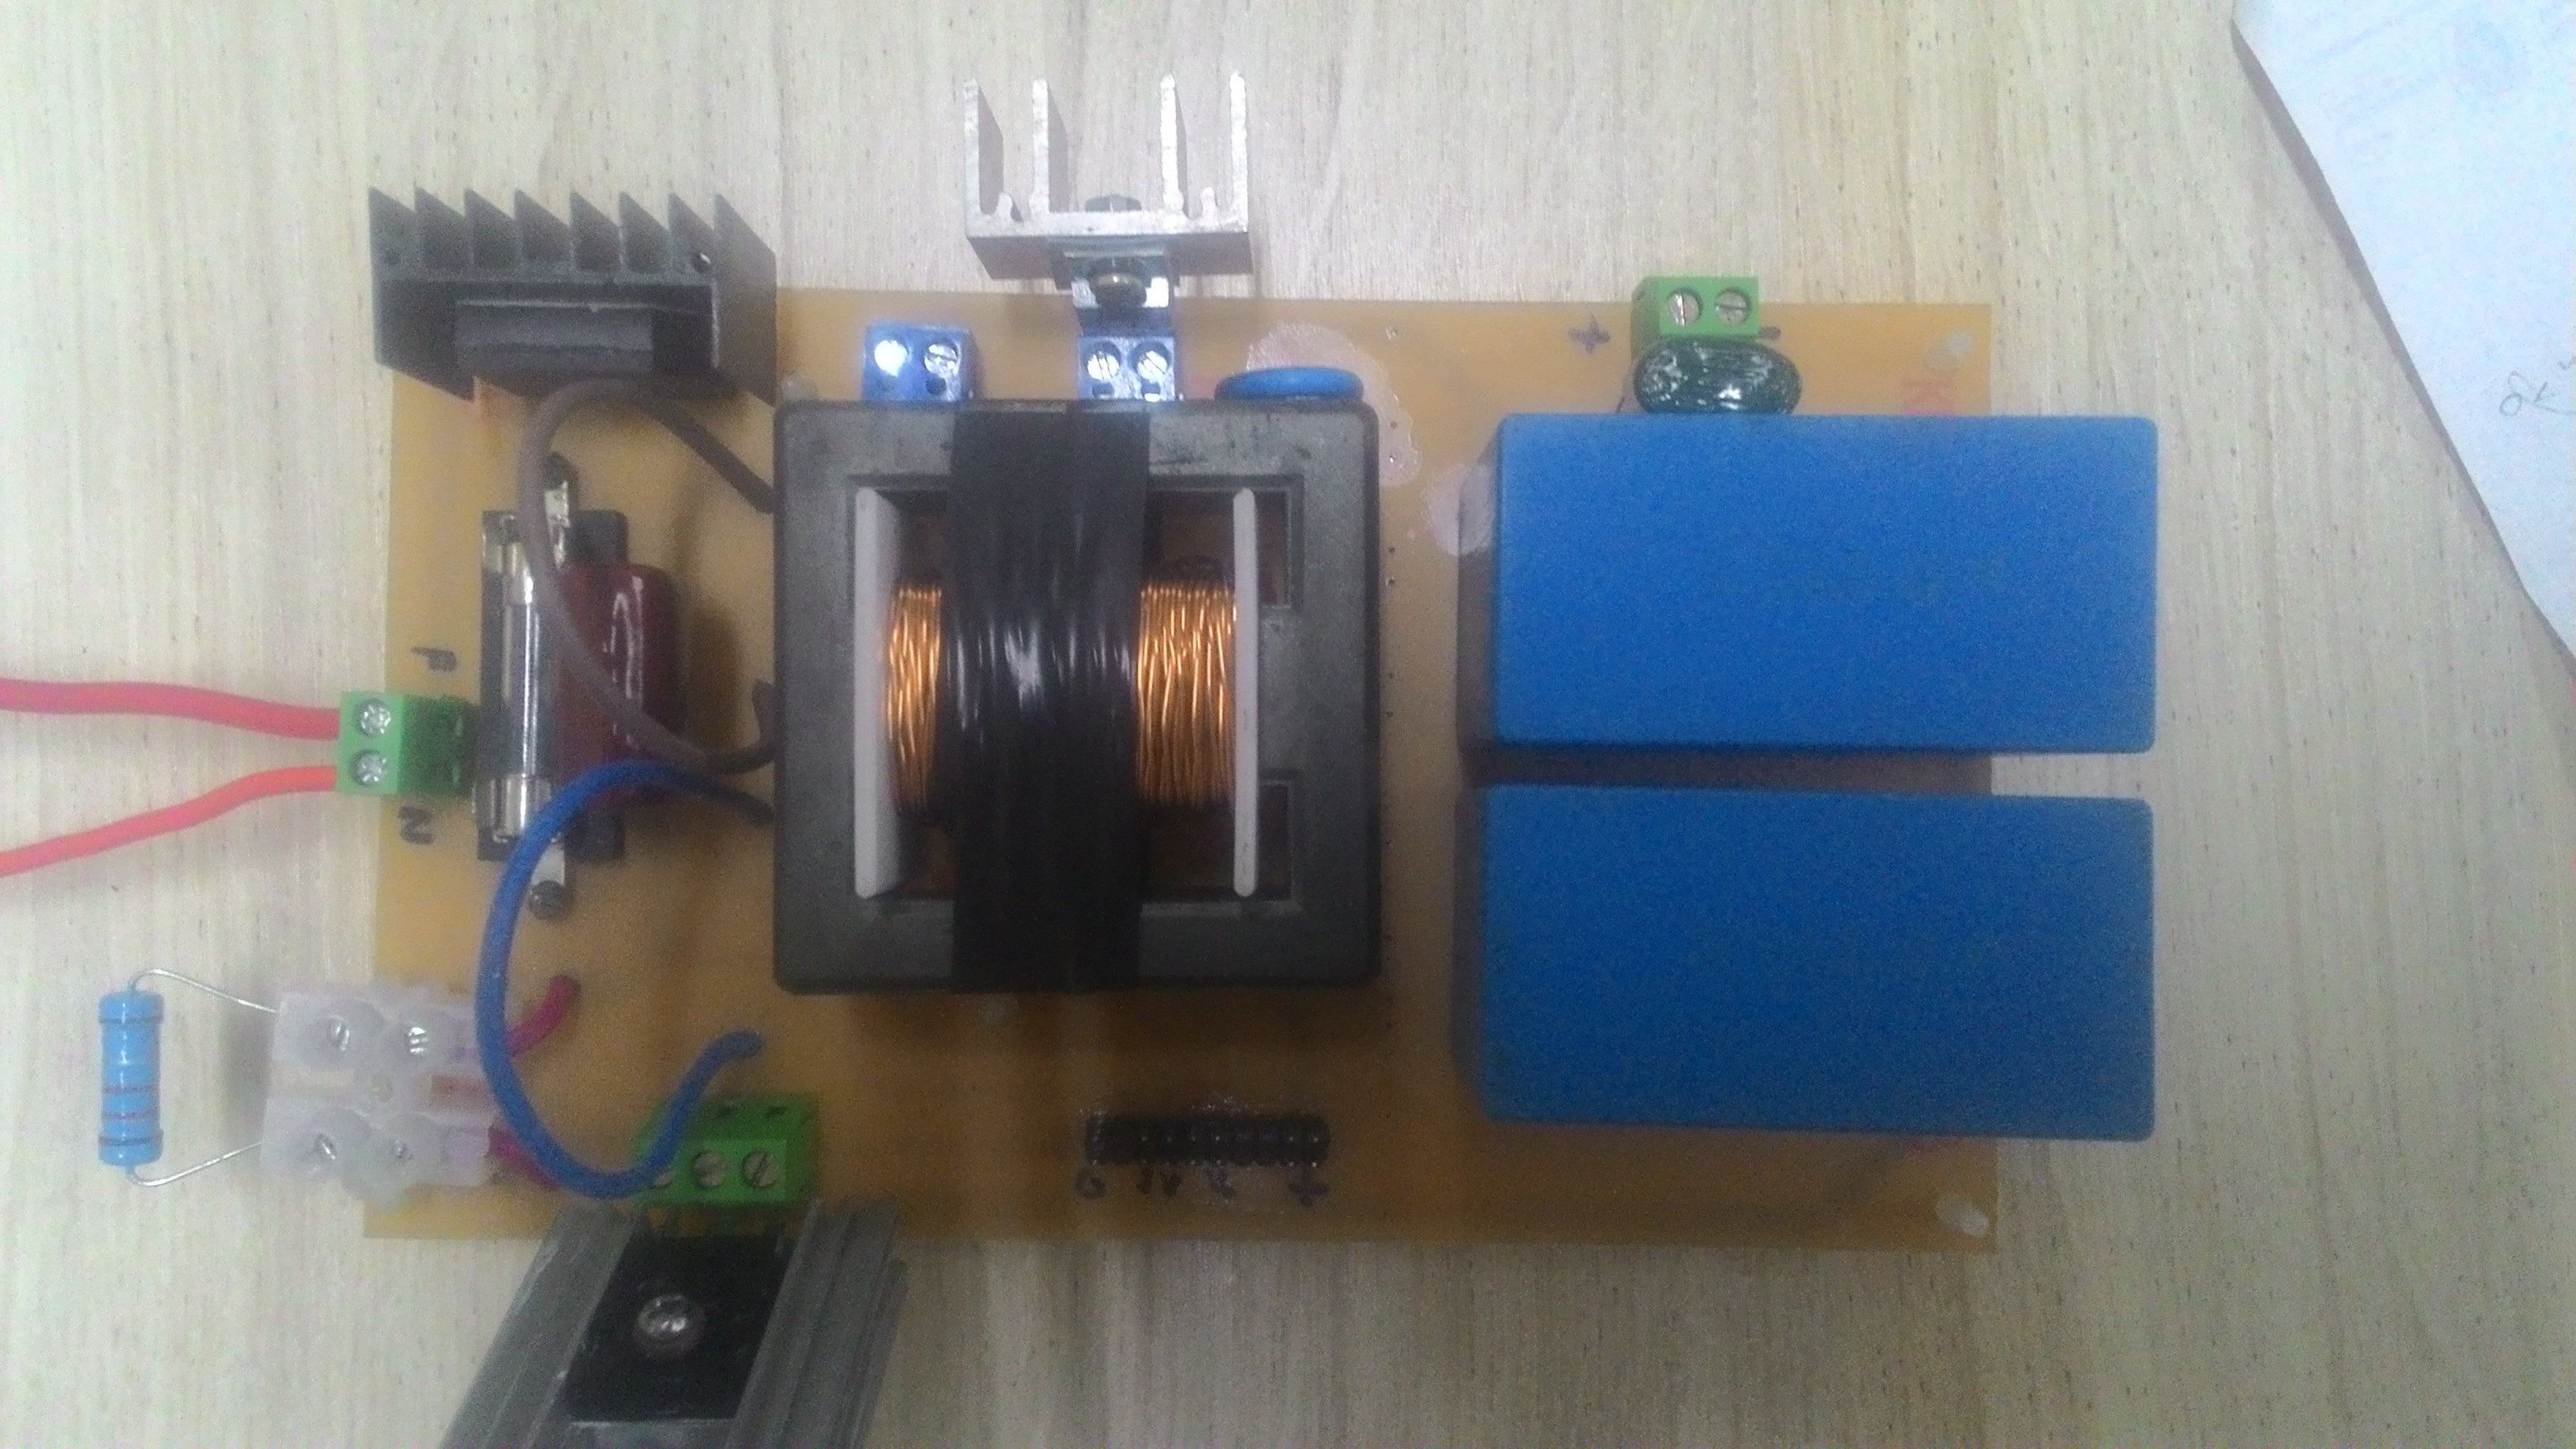
\includegraphics[scale=.05]{../FOTOGRAFIAS/P_20180910_174425.jpg}\\
	\fonte{Acervo Pessoal.}
\end{figure}


O sistema de controle foi primeiro testado usando montagem em protoboard, para ajuste dos parâmetros. Foi constatado que as equações da aplication note \cite{slua} e a simulação eram um bom ponto de partida, mas algumas pequenas modificações de valores em capacitâncias e resistências do circuito de controle se fizeram necessárias na prática, de forma a otimizar os resultados obtidos.

Os componentes que precisaram de ajuste foram $R_{pk2}$, limitador da corrente de pico, aumentado em 50\% por estar limitando demais, $R_{mo}$ e $R_{ci}$, malha de corrente, aumentado em 30\% porque não estavam permitindo o fluxo certo de potência, e $C_{vf}$, malha de tensão, dobrado para deixar a dinâmica mais lenta e limpar certo ruído que se manifestou, além de ajustes finos em $R_{vi}$ e $R_{vd}$ para chegar na tensão correta.

A placa de controle foi fabricada no Label em fibra de vidro face simples utilizando o método de transferência térmica e corrosão, sendo montada no NIMO.

\begin{figure}[!h]
	\centering
	\caption{Protótipo PFC - Placa de controle}
	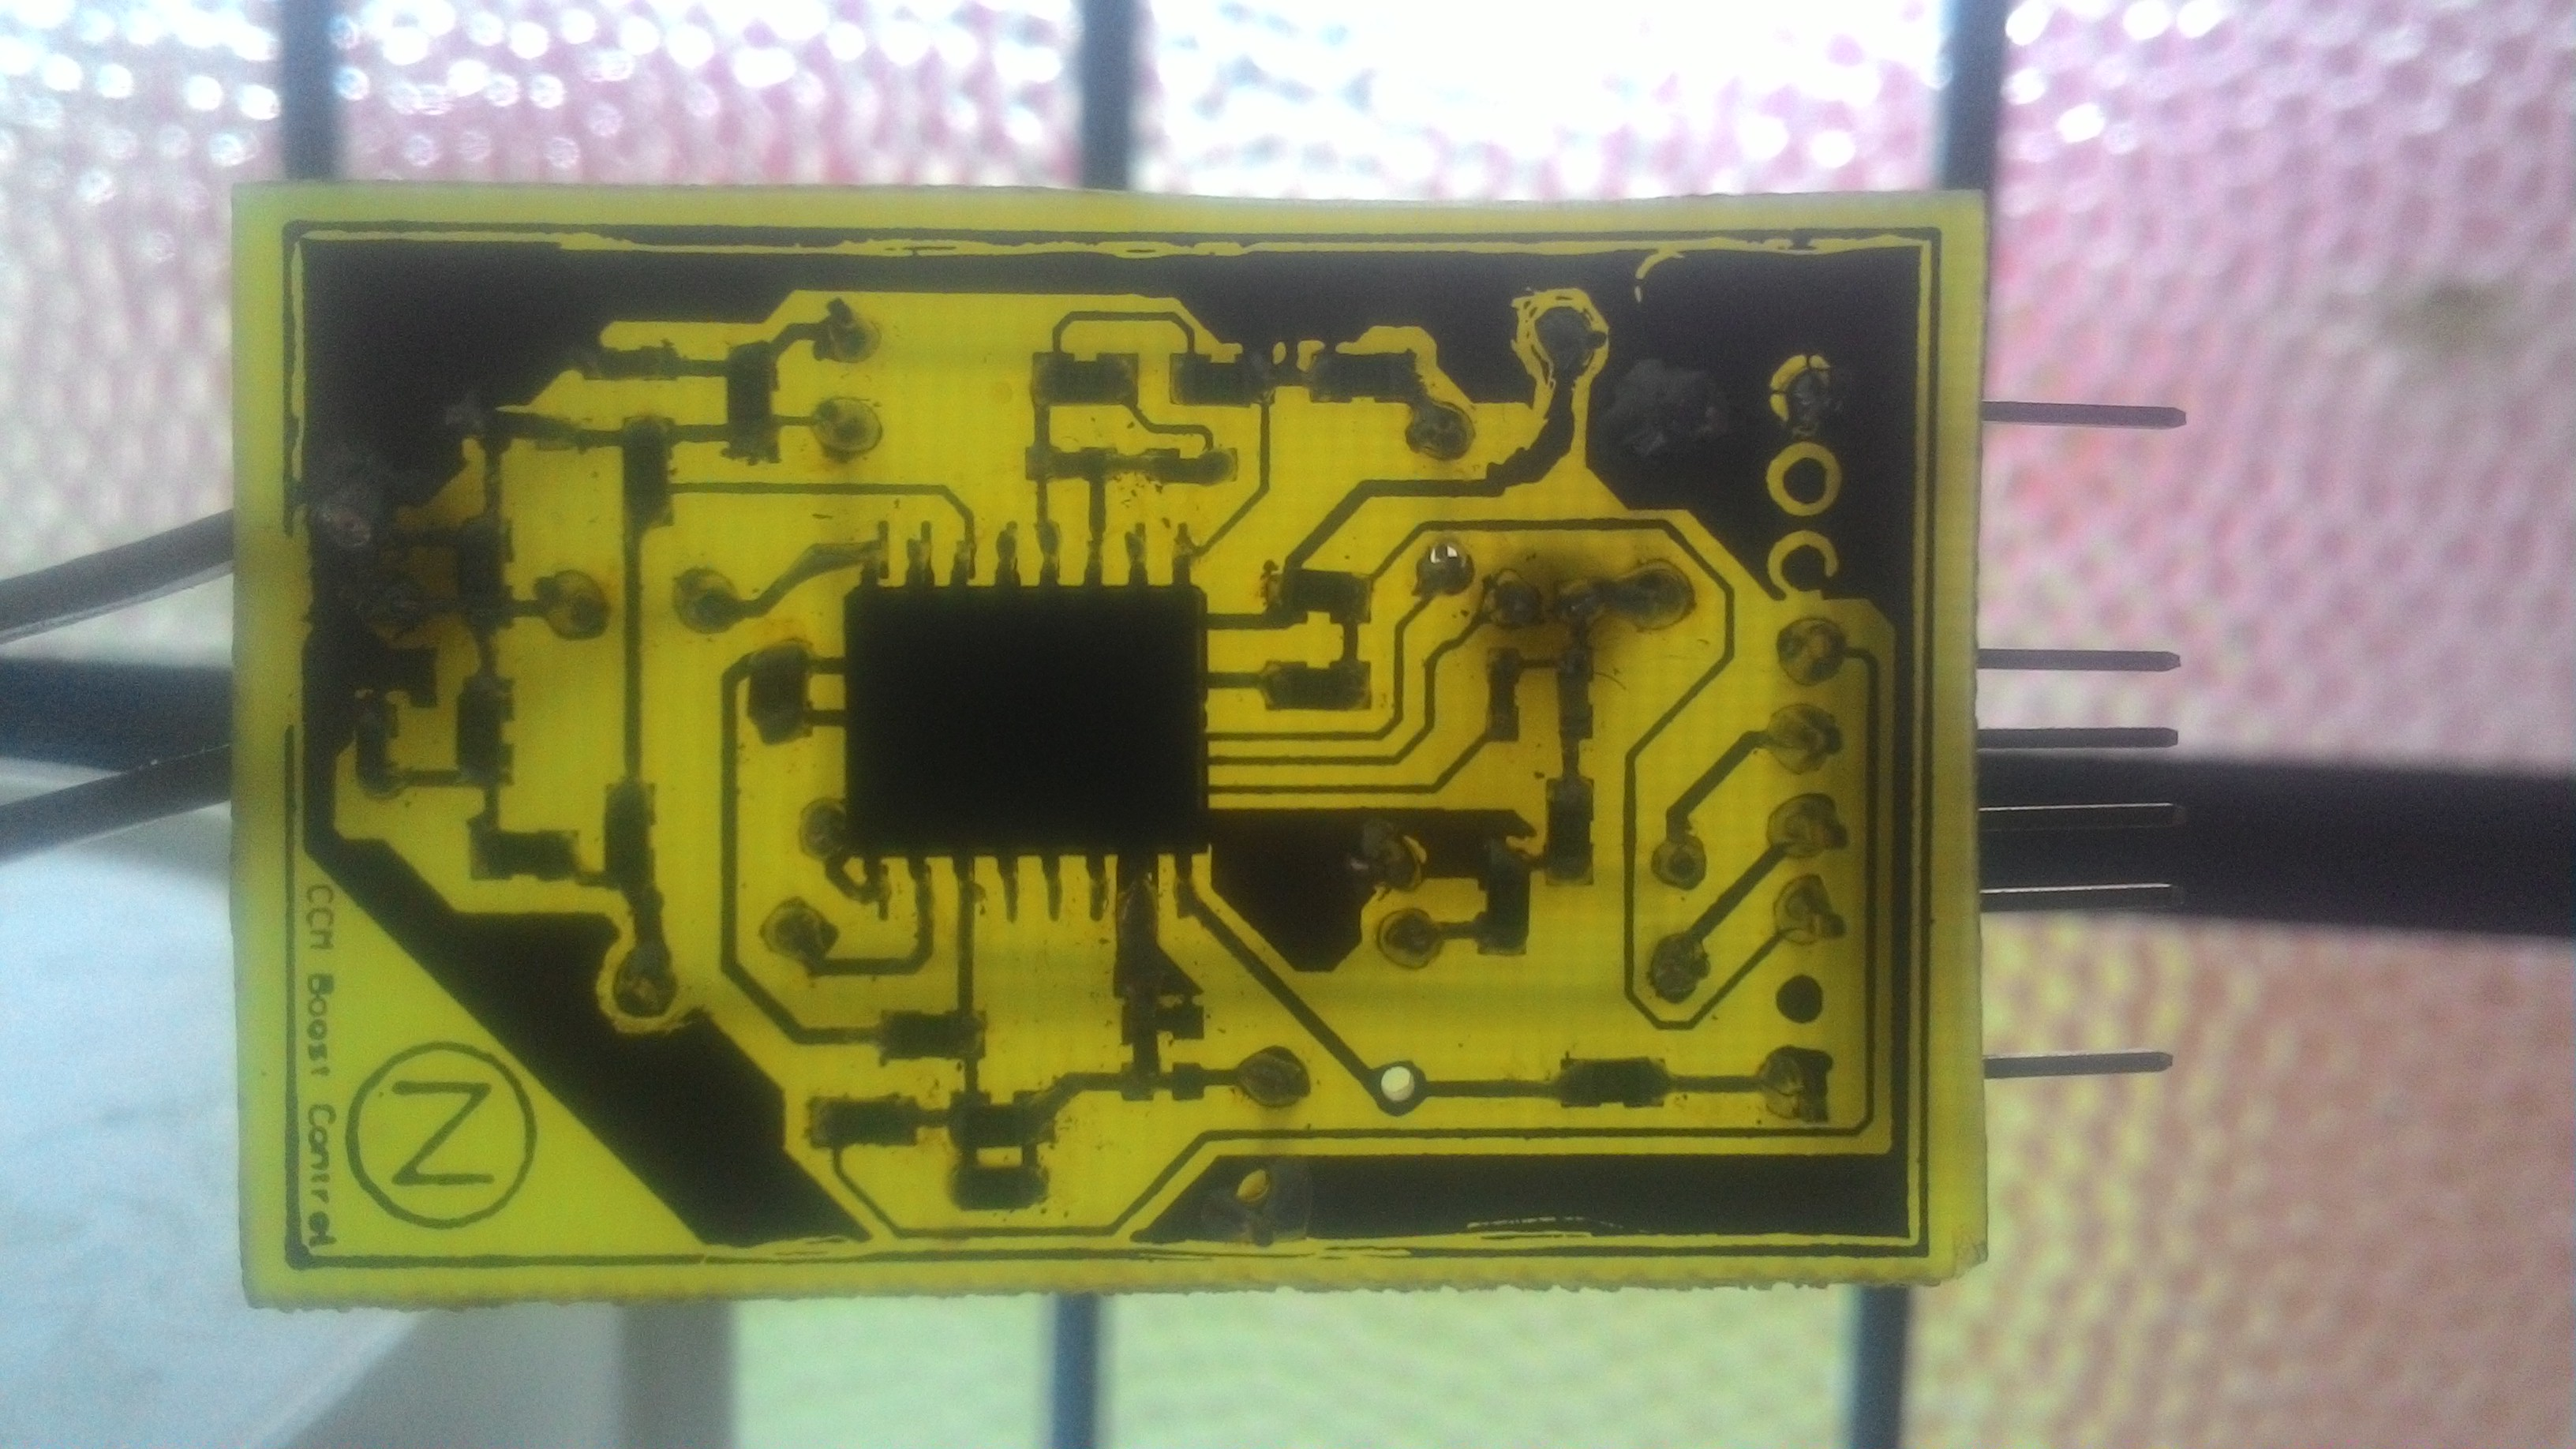
\includegraphics[scale=.05]{../FOTOGRAFIAS/P_20180910_103427.jpg}
	\fonte{Acervo Pessoal.}
\end{figure}

Após montado o conversor, este foi testado utilizando reostatos como carga, com a resistência equivalente do segundo estágio. O conversor foi alimentado usando a fonte California 5kW.


Na figura \ref{o_pfc_v_i_220}, são apresentadas a tensão de entrada, de $220V_{RMS}$, e a corrente de entrada do conversor \textit{boost} PFC. Constata-se que a corrente é senoidal, exceto por um baixo nível de distorção de alta frequência, e em fase com a tensão de entrada.

\begin{figure}[!h]
	\centering
	\caption{Formas de onda para o estágio PFC: Tensão nominal (azul) e corrente de entrada (vermelha).}
	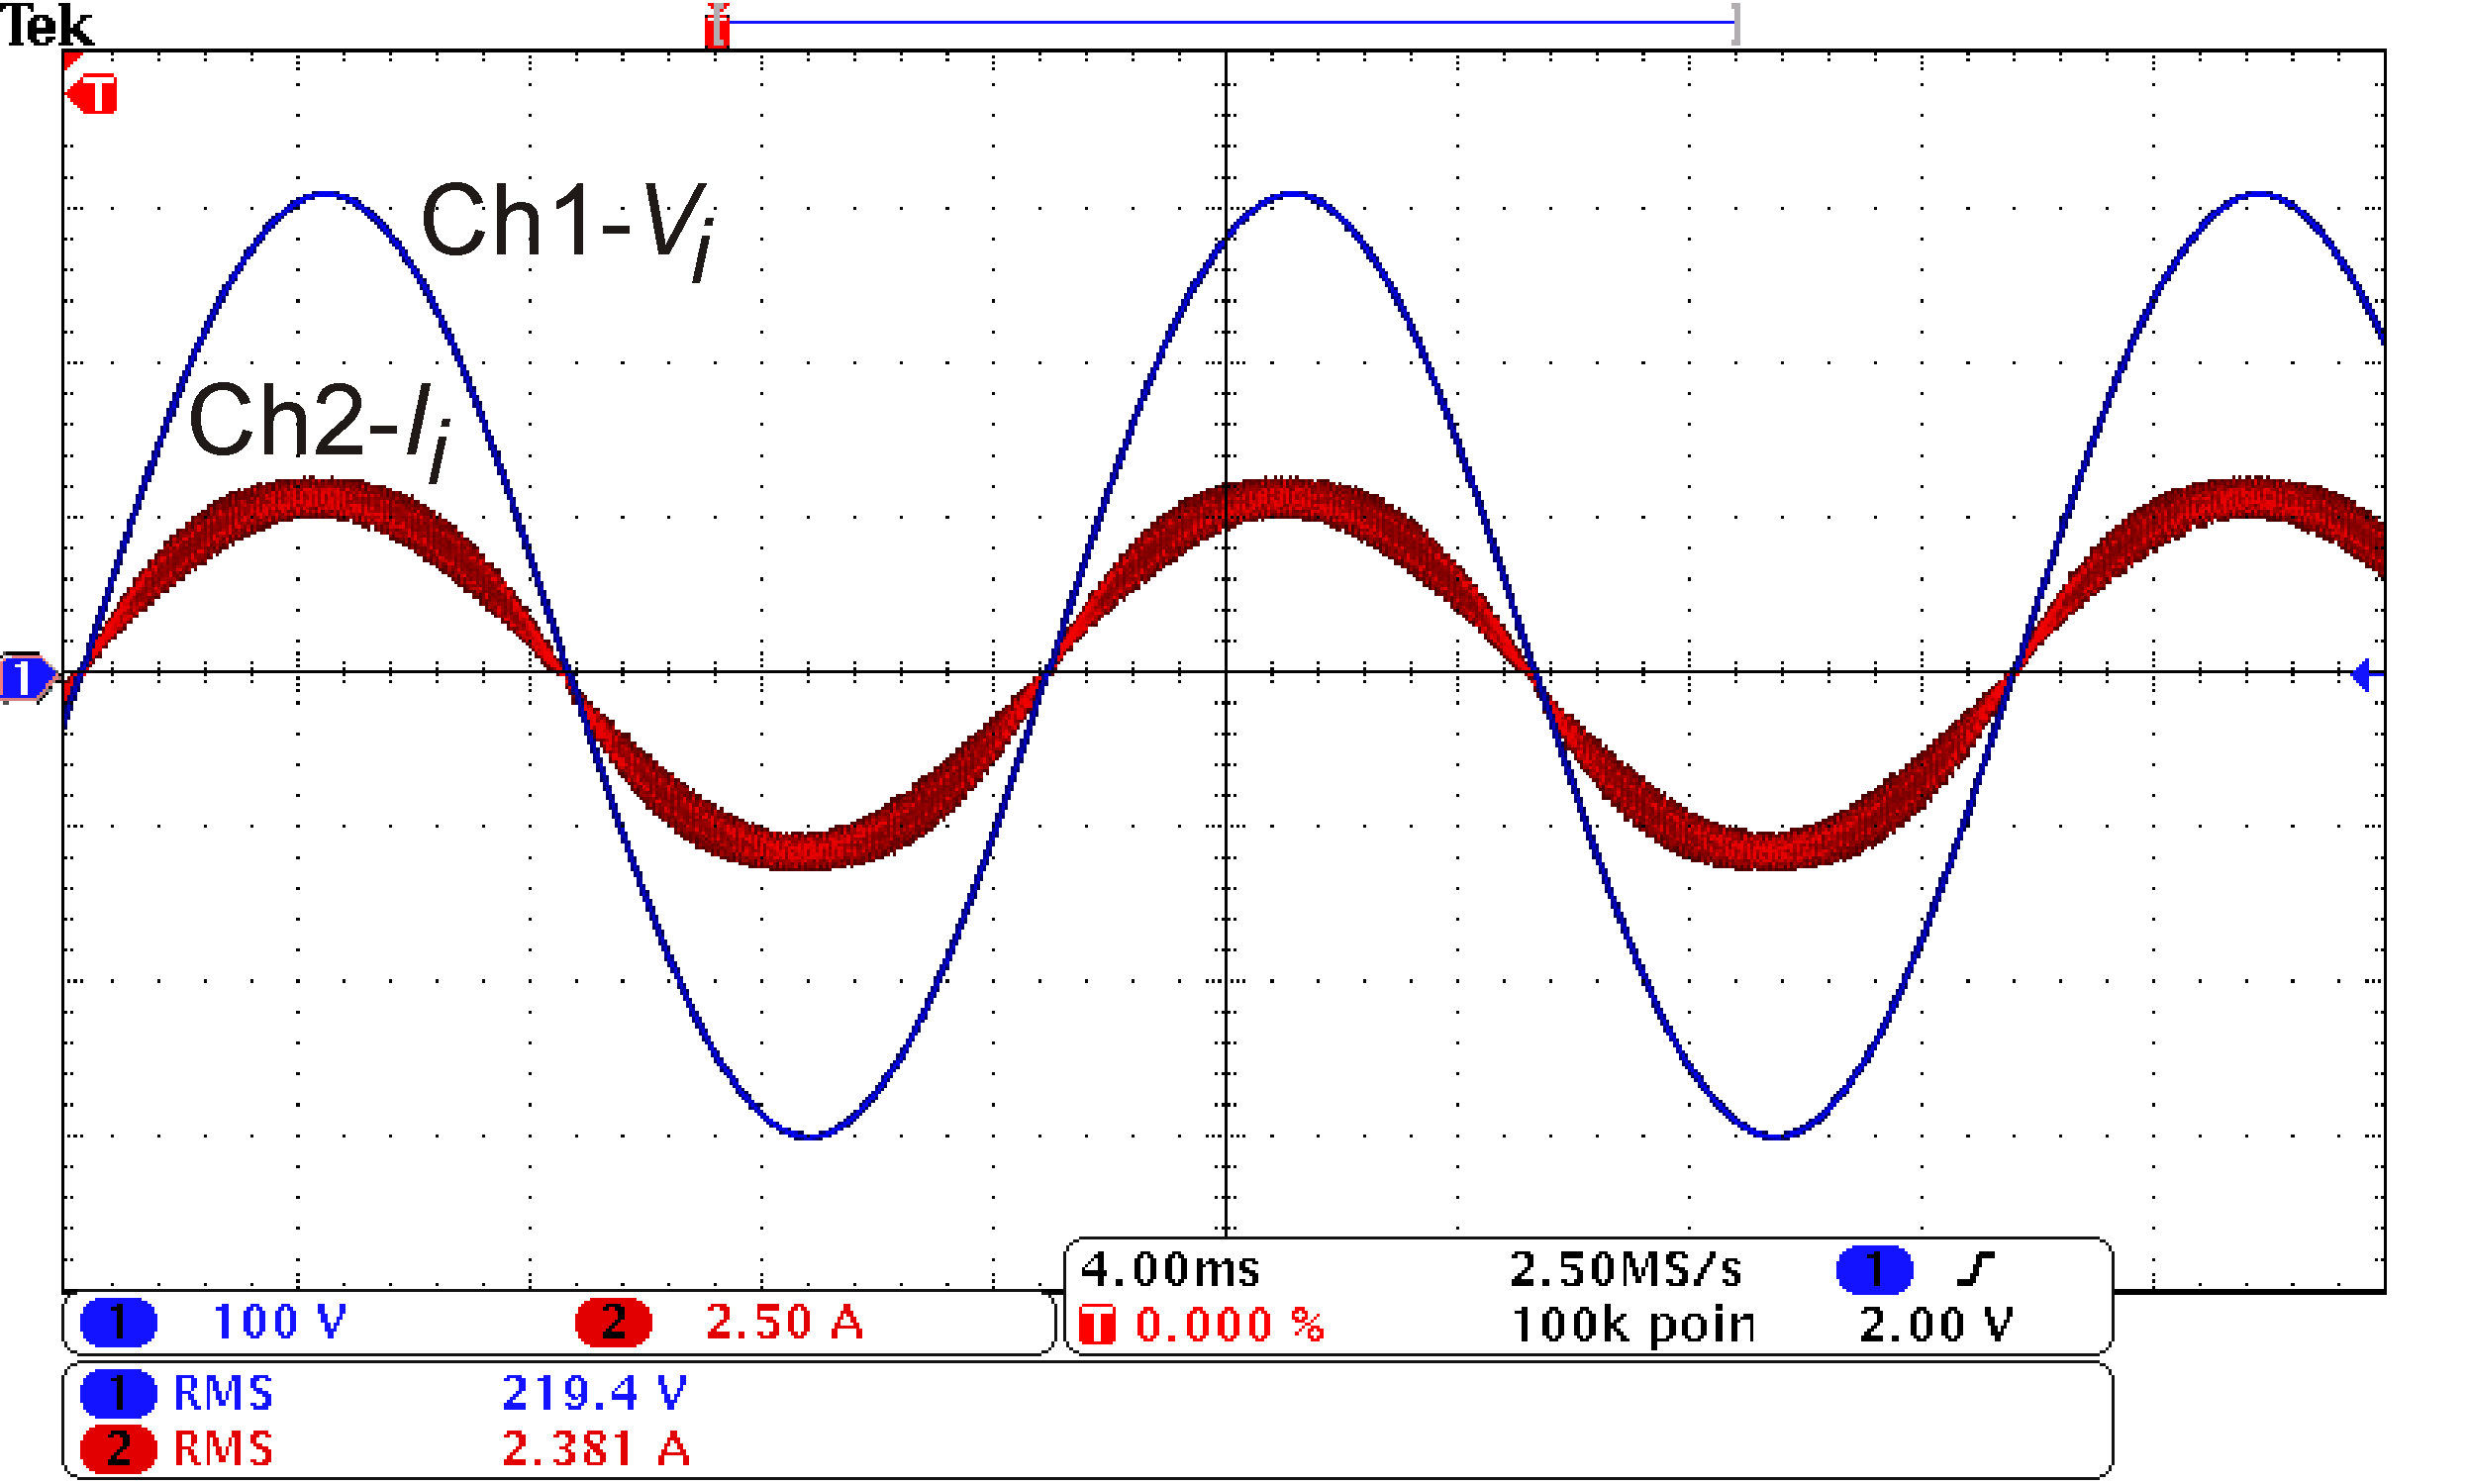
\includegraphics[width=0.7\linewidth]{../FIGURAS/Figuras_TFC_Eric/Formas_de_onda/PFC_ACM}
	\fonte{Fonte: Pereira, D. C. (2019) \cite{denis}.}
	\label{o_pfc_v_i_220}
\end{figure}

Na figura \ref{o_pfc_v_i} é mostrado o conversor operando em 127V. Constata-se que o projeto é funcional em tensão universal, sem maiores inconvenientes.

\begin{figure}[!h]
	\centering
	\caption{Formas de onda para o estágio PFC: Tensão em 127V (azul) e corrente de entrada (ciano).}
	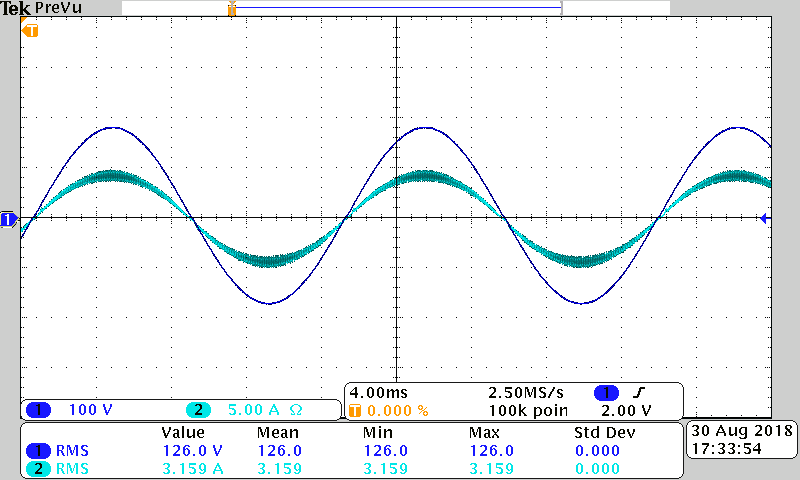
\includegraphics[width=0.7\linewidth]{../GRAFICOS/TEK/tek00042}
	\fonte{Acervo Pessoal.}
	\label{o_pfc_v_i}
\end{figure}



Na forma de onda da figura \ref{o_pfc_ind}, é vista uma captura com a corrente no indutor, modulada em uma senóide retificada. Além disso, nesta figura é apresentada também a forma de onda da tensão no barramento, que é próxima a 400 V com 20 V pico a pico de ondulação de baixa frequência.

\begin{figure}[!h]
	\centering
	\caption{Formas de onda para o estágio PFC: corrente no indutor (ciano) e tensão de saída (azul).}
	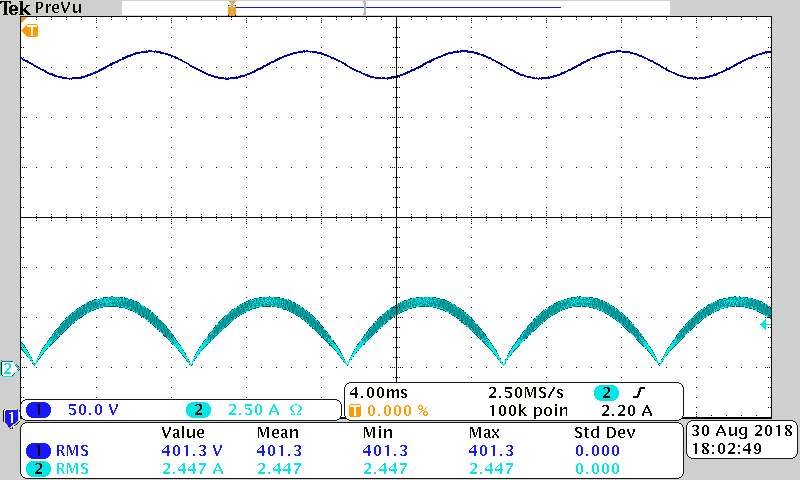
\includegraphics[width=0.7\linewidth]{../GRAFICOS/TEK/tek00064}
	\fonte{Acervo Pessoal.}
	\label{o_pfc_ind}
\end{figure}




Na captura da figura \ref{o_pfc_ctrl}, o conversor é submetido a uma variação na tensão de entrada de 10\%. Pode-se ver que o comportamento transitório é satisfatório, tendo um retorno suave.

\begin{figure}[!h]
	\centering
	\caption{Conversor PFC submetido a distúrbio na tensão de entrada. Formas de onda para a corrente de entrada (ciano) e tensão no barramento (azul).}
	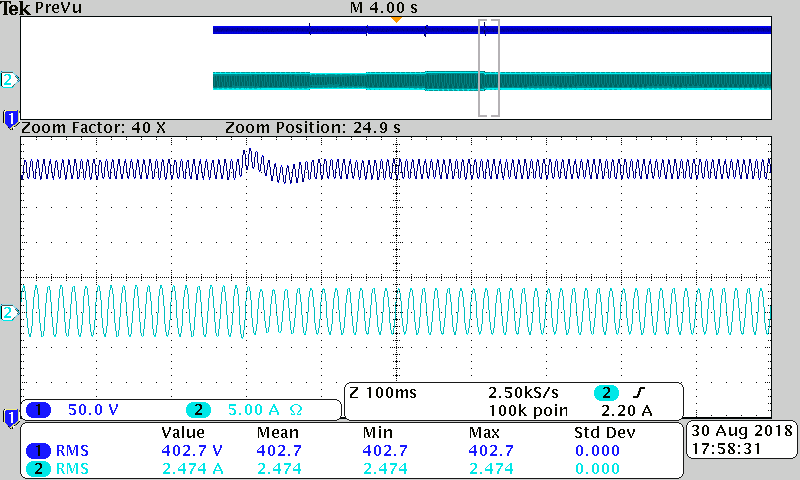
\includegraphics[width=0.7\linewidth]{../GRAFICOS/TEK/tek00058}
	\fonte{Acervo Pessoal.}
	\label{o_pfc_ctrl}
\end{figure}


A eficiência deste estágio isolado foi medida com o watímetro digital Yokogawa em 96\%, quando operando com tensão de entrada de $220V_{rms}$ como mostrado na Figura \ref{yoko}. O fator de potência foi praticamente unitário.

\begin{figure}[!h]
	\centering
	\caption{Protótipo PFC - Leituras do wattímetro}
	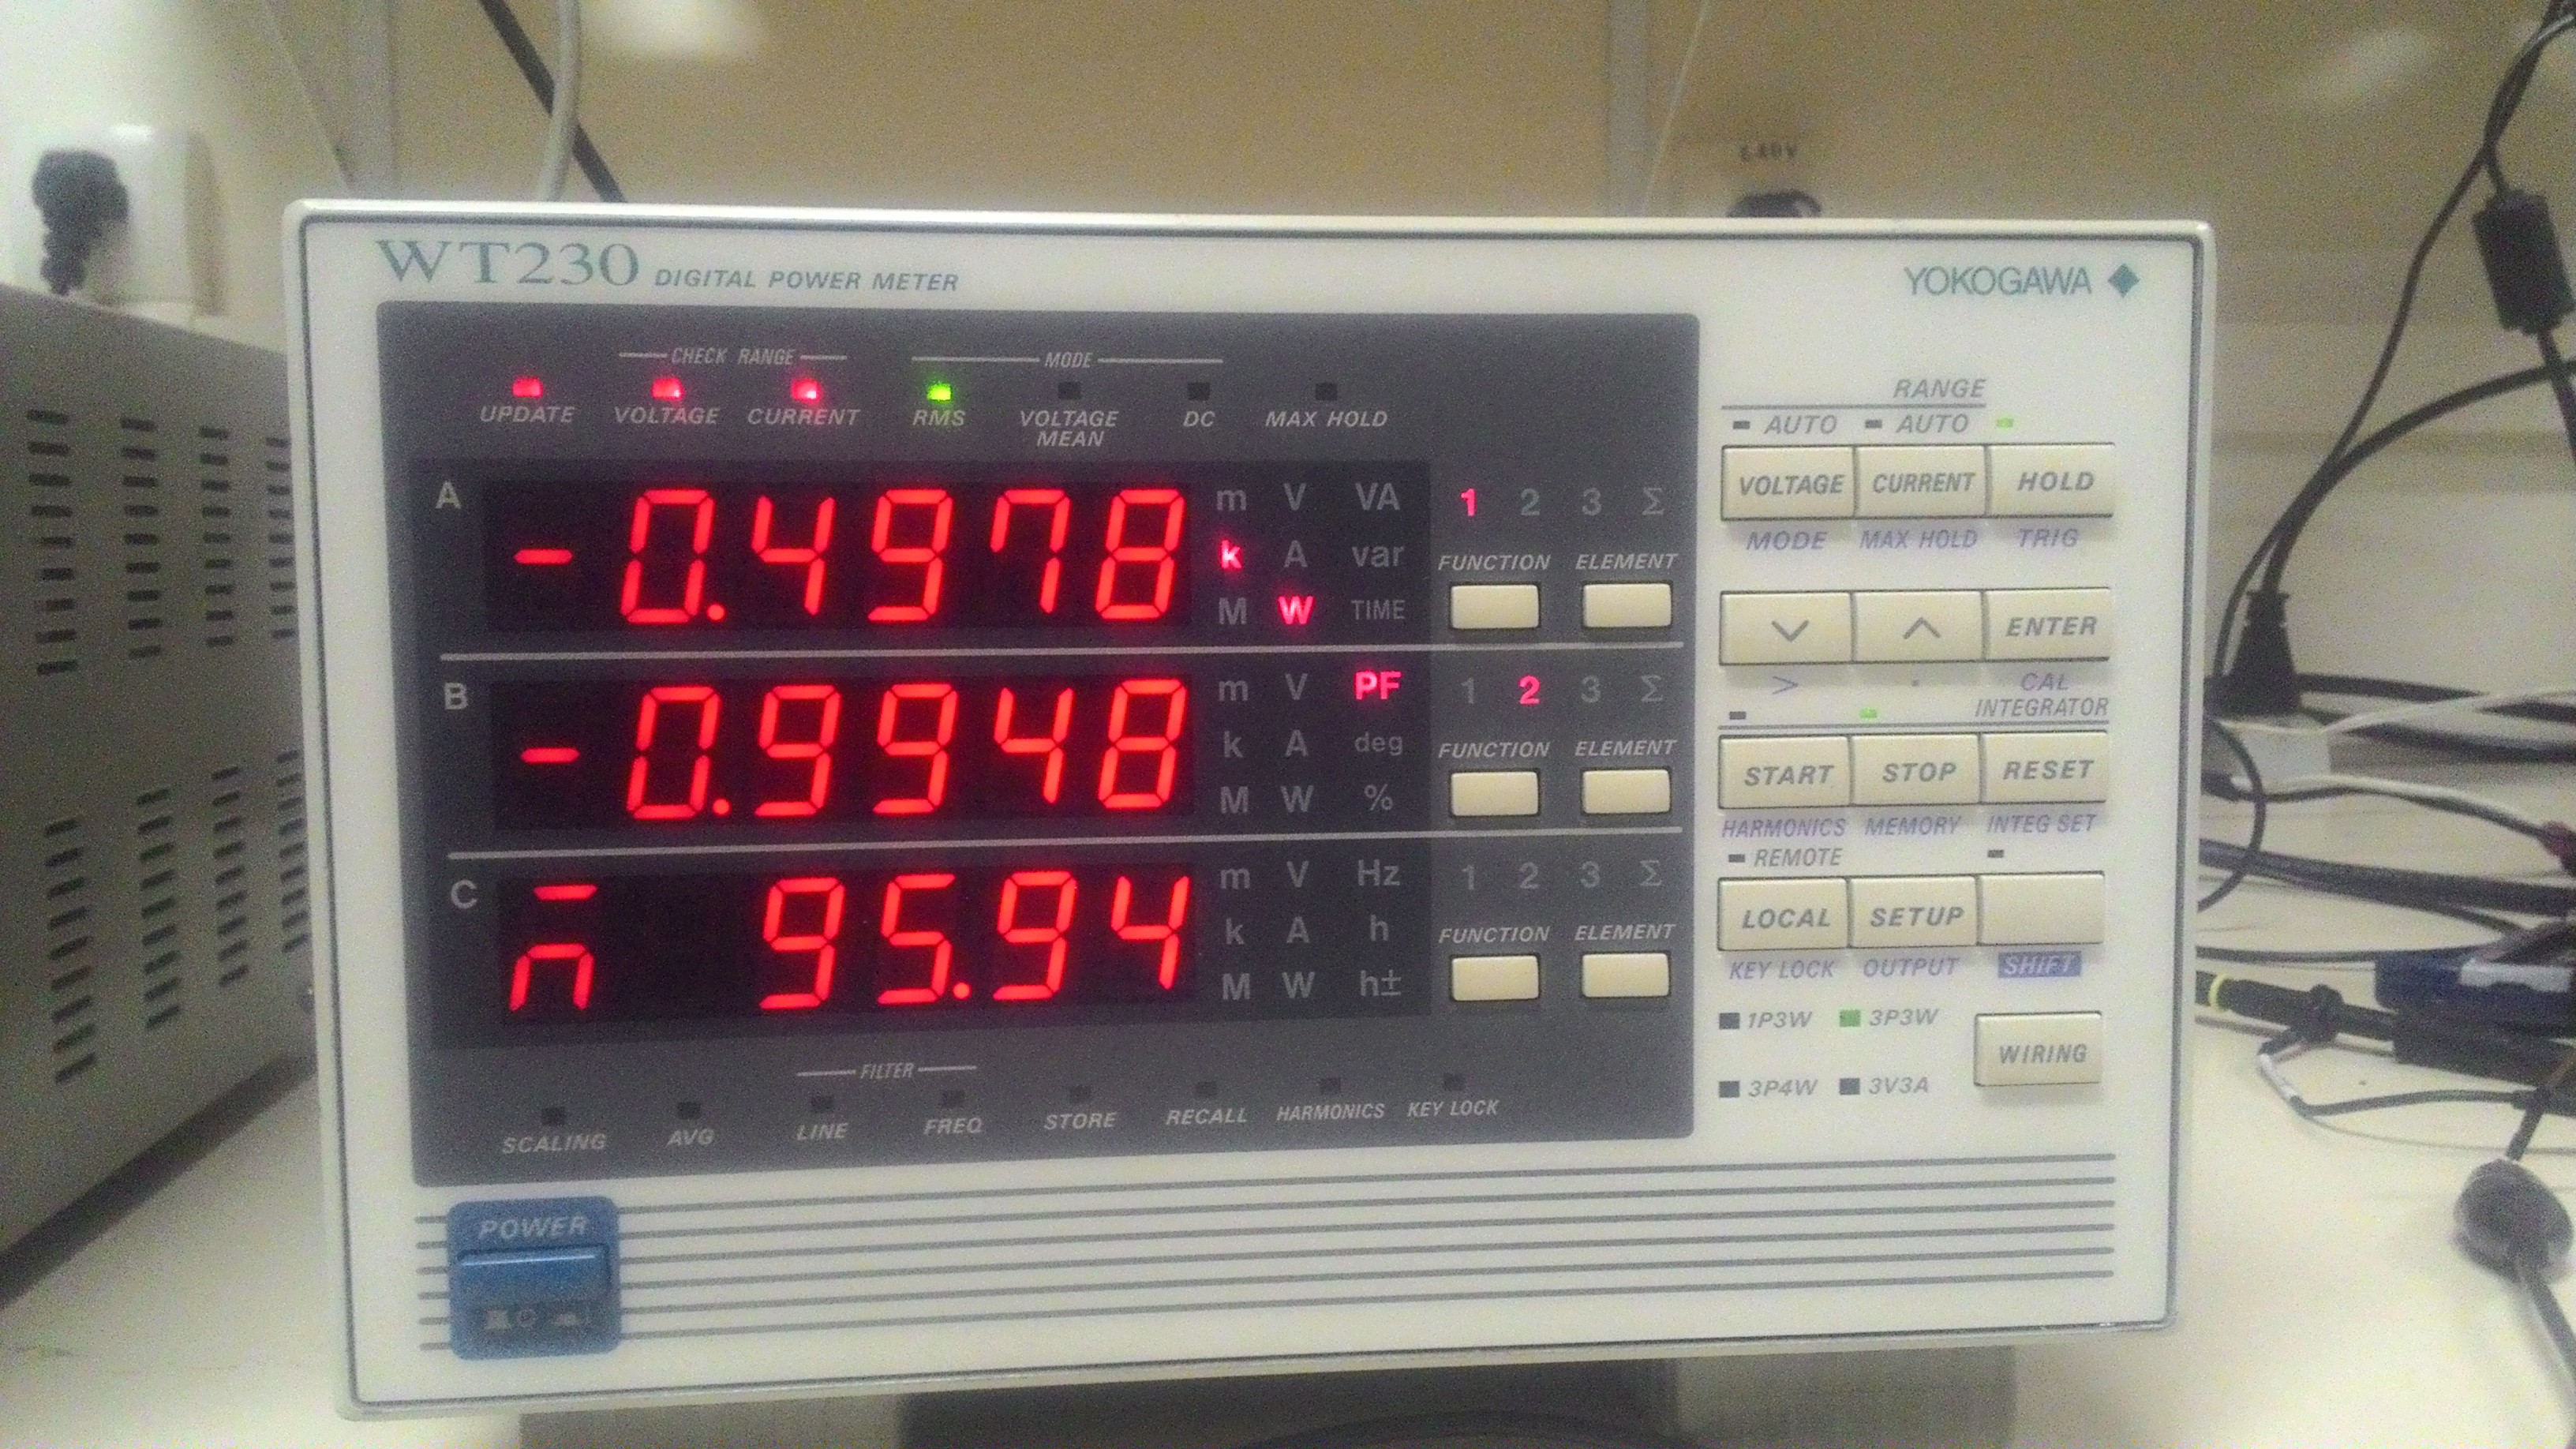
\includegraphics[scale=.05]{../FOTOGRAFIAS/P_20180830_175245.jpg}\\
	\fonte{Acervo Pessoal.}
	\label{yoko}
\end{figure}


\section{Segundo estágio}

Cronologicamente, o primeiro conversor montado foi o EDSCIBC, protótipo apresentado na Figura 40. Os dois indutores foram construídos em núcleo E modelo NEE 42-21-20, 40 voltas. Foi constatado que o máximo fio que poderia ser usado na frequência de 40kHz era o AWG 22, devido à questões relacionadas ao efeito \textit{skin} de acordo com a profundidade de penetração e condução da corrente no fio escolhido, se fazendo necessário o uso de três fios entrelaçados para garantir a ampacidade necessária. O restante dos componentes, os capacitores série e de saída; os MOSFETs e diodos, são de mercado, sendo que os seus respectivos valores e modelos são mostrados na Tabela \ref{pc-matlist}.




\begin{table}[]
	\centering
\caption[Indutores, capacitores e modelos dos semicondutores utilizados no protótipo do conversor EDSCIBC PC.]{
	\parbox[t]{10cm}{Indutores, capacitores e modelos dos semicondutores utilizados no protótipo do conversor EDSCIBC PC.}}
	\begin{tabular}{|l|l|}
		\hline
		Indutores                      & 500 $\mu H$ \\ \hline
		Capacitor série de acoplamento & 12 $\mu F$   \\ \hline
		Capacitor de saída             & 40 $\mu F$    \\ \hline
		MOSFETs S1 e S2                & IRFP460    \\ \hline
		Diodos D1 e D2                 & MUR 8100   \\ \hline
	\end{tabular}
	\label{pc-matlist}
\end{table}

A placa de circuito, de face simples, foi fabricada no Laboratório de Processos da UFJF com uma CNC LPKF\textregistered. O conversor, apresentado em \ref{pc-board}, foi montado no NIMO.

\begin{figure}[!h]
	\centering
	\caption{Protótipo PC - Placa de potência}
	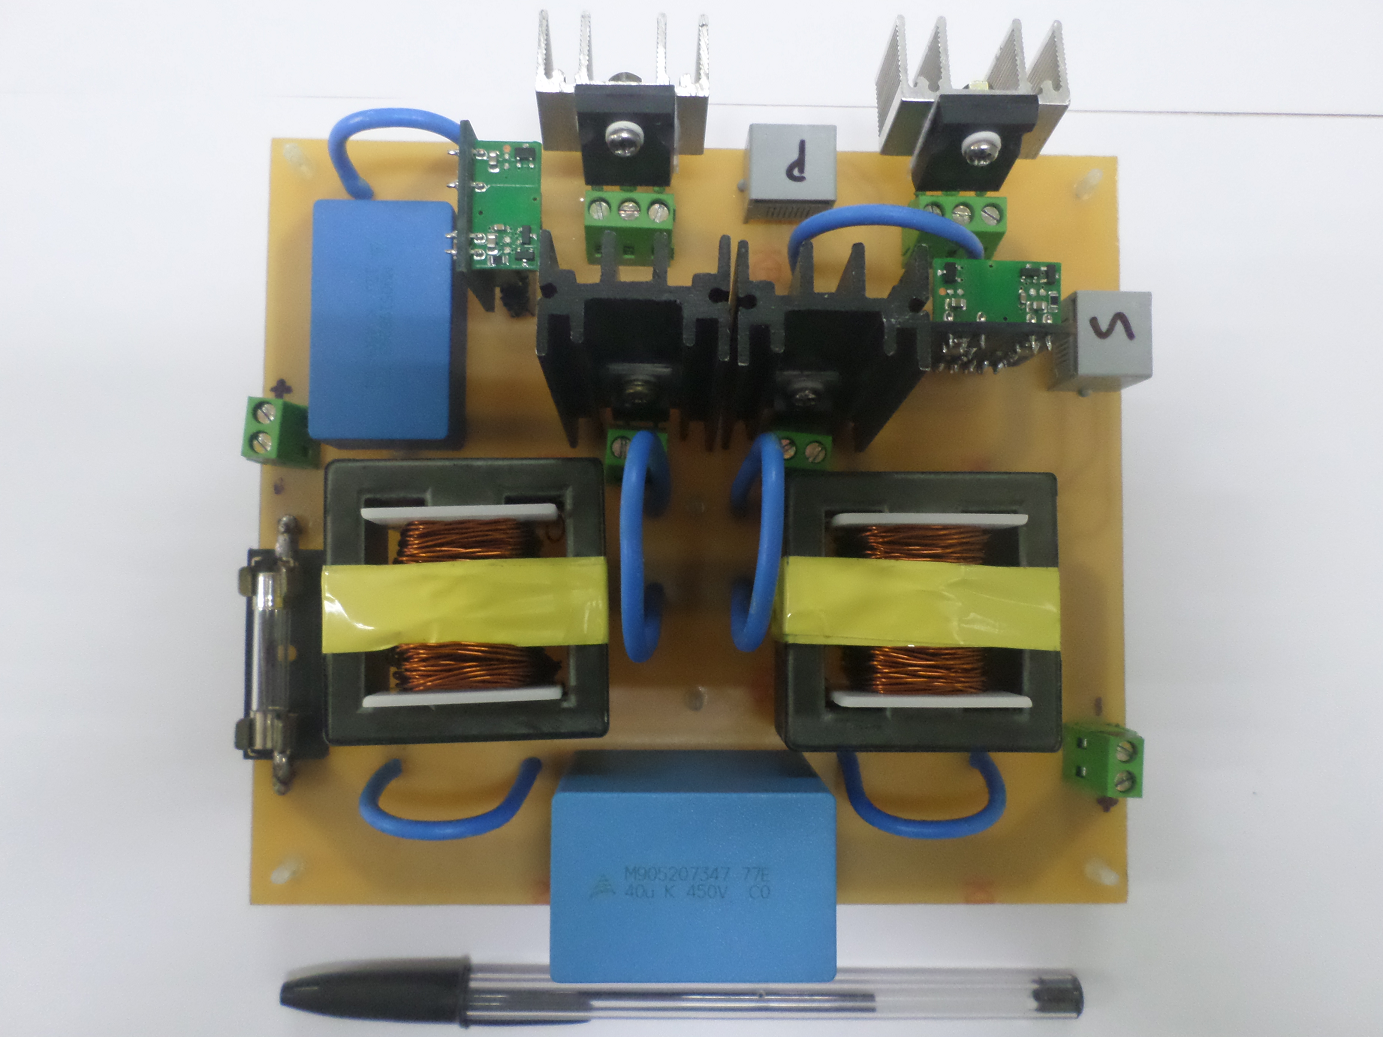
\includegraphics[scale=.16]{../FOTOGRAFIAS/D1.png}\\
	\fonte{Acervo Pessoal.}
	\label{pc-board}
\end{figure}

Os sinais de acionamento e sensoriamento foram roteados a partir e para a placa de controle com cabos de rede e conectores RJ45, conforme apresentado na foto da figura \ref{pc-ctrl-board}. O controle foi implementado digitalmente em uma placa de prototipagem Tiva-C da Texas Instruments\textregistered. A placa é equipada com um microcontrolador TM4c123gh6pm, que conta com CPU Cortex\textregistered ~M4 de 80 MHz, ADC de 12 bits e contadores de 16 bits com múltiplas configurações de geração de onda. Para o interfaceamento, foi feita uma placa \textit{dock} roteando os sinais para os conectores de rede.

O programa embarcado no processador se utiliza de uma interrupção configurada no \textit{overflow} do contador onde o sinal PWM é gerado, que é o momento central entre a abertura e o fechamento de um dos interruptores, o local com menor ruído possível para fazer a amostragem. O \textit{trigger} gerado pela interrupção é direcionado ao ADC, o que inicia uma conversão, que é lida pela CPU. É feita a sequência de cálculo descrita na seção 3.3 e o valor resultante é escrito no registrador, que é usado pelo módulo PWM para definir a largura de pulso. O código usado pode ser consultado em \cite{github}. 

\begin{figure}[!h]
	\centering
	\caption{Protótipo PC - Microcontrolador conectado à placa dock e respectivas ligações de sensoriamento e sinais PWM para os interruptores do estágio PC.}
	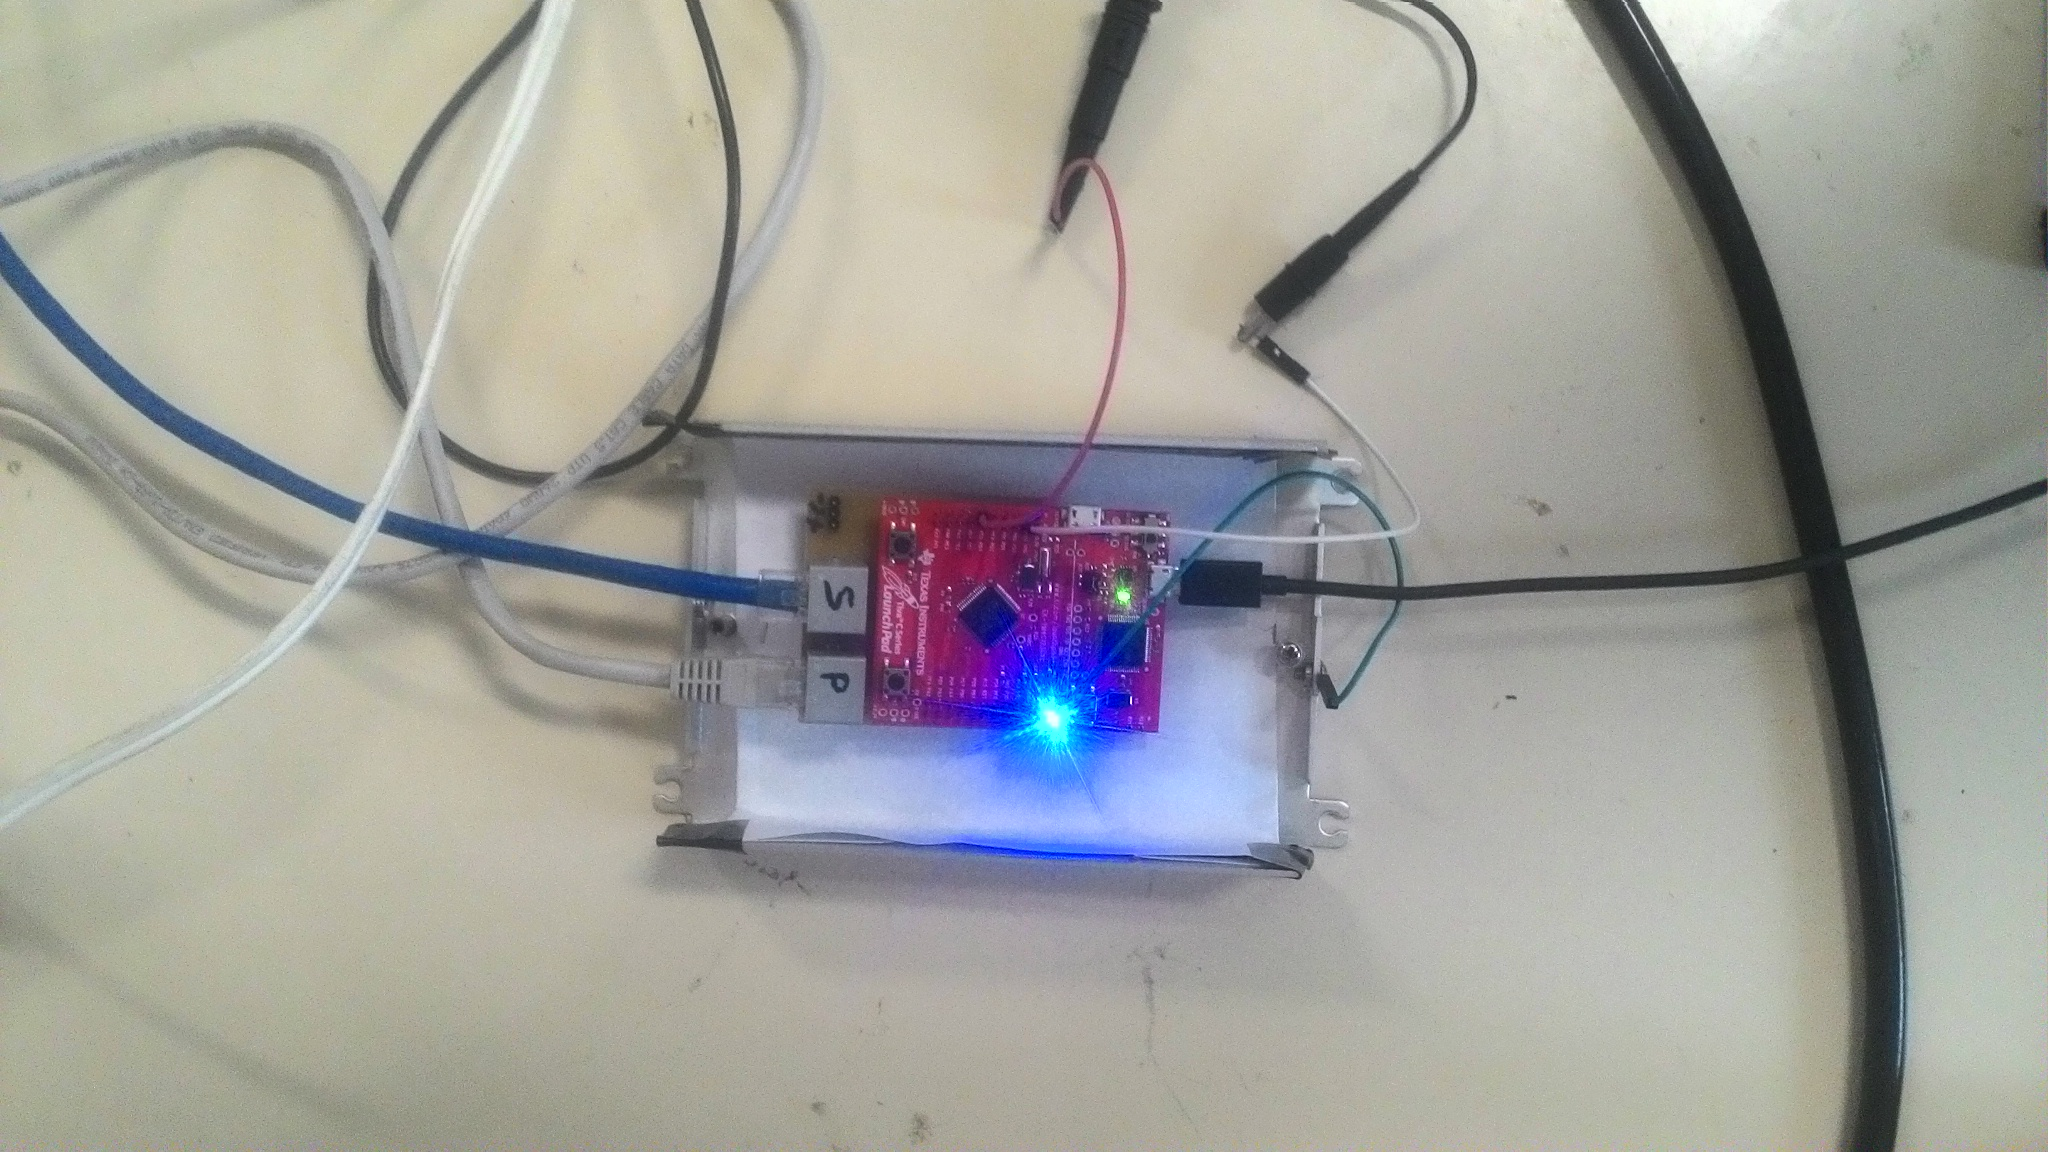
\includegraphics[scale=.1]{../FOTOGRAFIAS/P_20180712_152414.jpg}\\
	\fonte{Acervo Pessoal.}
	\label{pc-ctrl-board}
\end{figure}


O acionamento dos MOSFETs foi feito usando uma placa projetada em \cite{livinha}, em um trabalho voltado a acelerar o desenvolvimento de protótipos dentro do laboratório. A placa foi fabricada no NIMO usando uma CNC industrial e coberta com máscara de solda de tinta fotossenssível.% na Casa do Vinícius.

%:plaquinha do vinicius

O sensoriamento da corrente foi feito usando o sensor de Efeito Hall ACS-712-20A \cite{acs}, fundo de escala de 20A, encapsulamento soic-4. O sensor conta com isolamento galvânico entre a entrada de corrente e a saída analógica. Foi usado um divisor resistivo para adequar a saída do sensor, de até 5V, ao range do ADC do processador, de 3,3V. A Figura \ref{acs-board} mostra uma tomada do circuito de sensoriamento de corrente de saída usando o ACS-712.


\begin{figure}[!h]
	\centering
	\caption{Protótipo PC - Sensor de corrente ACS-712 na placa de potência}
	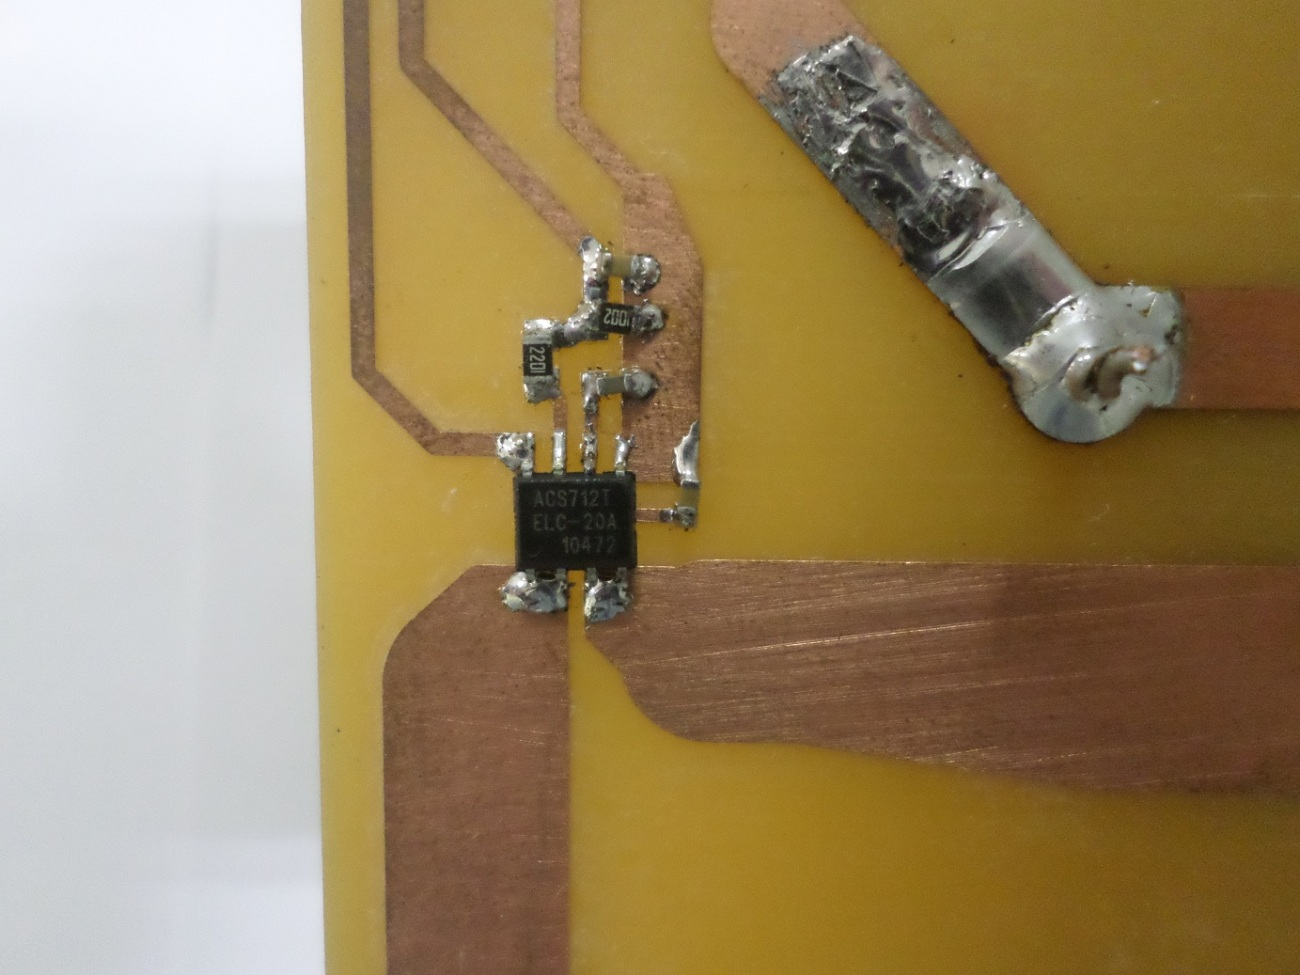
\includegraphics[scale=.3]{../FOTOGRAFIAS/D2.jpg}\\
	\fonte{Acervo Pessoal.}
	\label{acs-board}
\end{figure}

%O controle foi implementado de forma digital, utilizando para isso uma placa tiva-C, da texas. Como sensor de corrente, foi usado um medidor de efeito Hall isolado de encapsulamento soic-4, o ALS329.

O conversor foi testado com auxílio da fonte California 5kW. Os instrumentos de medida foram o Watímetro YOKOGAWA WT-230, Osciloscópio Tectronix, pontas de prova isoladas de tensão e corrente. Em testes preliminares foram usados reostatos para emular a mesma condição de corrente na saída do circuito, de forma a poupar o COB LED de possíveis danos por erro humano.

No decorrer dos testes, foi constatada a necessidade de um \textit{snubber} em um dos diodos, para atenuar um pico de tensão que se fazia presente. Este foi implementado em topologia RCD, com um resistor de porcelana de 4,7 k$\Omega$ 10W e um capacitor de disco cerâmico de 1 nF 4 kV. Também foi preciso adicionar um filtro de linha LC na placa \textit{dock}, na trilha de sensoreamento do conversor, em série com a linha de sinal, pois o microcontrolador estava sendo desligado devido a um circuito de proteção interna, sendo sensibilizado por surtos de tensão extremamente curtos transferidos à linha de sensoriamento, provavelmente por acoplamento indutivo.

%Na captura do osciloscópio mostrada na figura \ref{o_pc_sems} é representada a tensão e corrente no interruptor S1, ainda sem o \textit{snubber}. É notável o tamanho dos picos causados pela comutação, tornando necessária a utilização de um \textit{snubber}.

%\begin{figure}[!h]
%	\centering
%	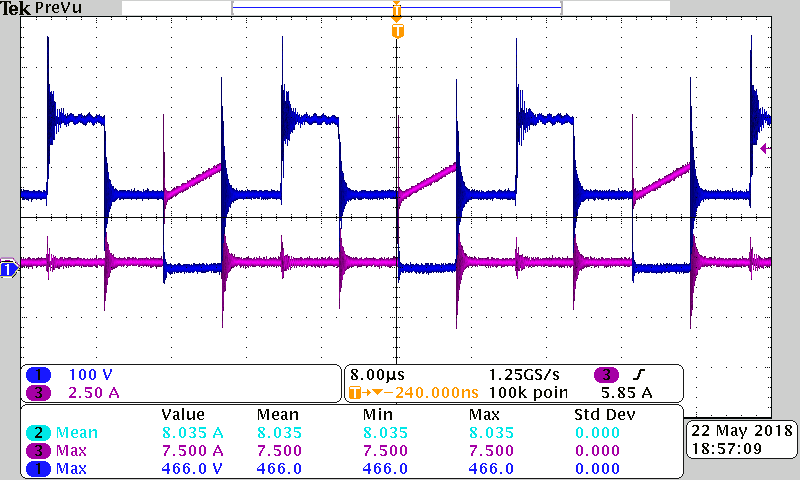
\includegraphics[width=0.7\linewidth]{../GRAFICOS/TEK/tek0020}
%	\caption{}
%	\fonte{Acervo Pessoal.}
%	\label{o_pc_sems}
%\end{figure}

%[não tenho figura dele bom, Denis... Não sei o que eu arrumei com elas]

%:operação normal

Nas figuras \ref{pc_wav_0} e \ref{pc_wav_1}, são mostrados os esforços nos diodos e nos MOSFETs, respectivamente. Constata-se que são da forma e intensidade previstas em projeto. Na figura \ref{pc_wav_88}, são apresentadas as formas de onda das correntes nos indutores, as quais estão em bom equilíbrio, com valores médios de 5A. Adicionalmente, as formas de onda das tensões gate-source dos MOSFETs também são mostradas na Figura \ref{pc_wav_88}, com as quais pode ser notado que o conversor opera com razão cíclica estendida, isto é, 0,25 para o ponto de operação deste trabalho.



\begin{figure}[!h]
	\centering
	\caption{Formas de onda para o estágio PC: Correntes (verde e vermelho) e tensões (azul e lilás) nos diodos.}
	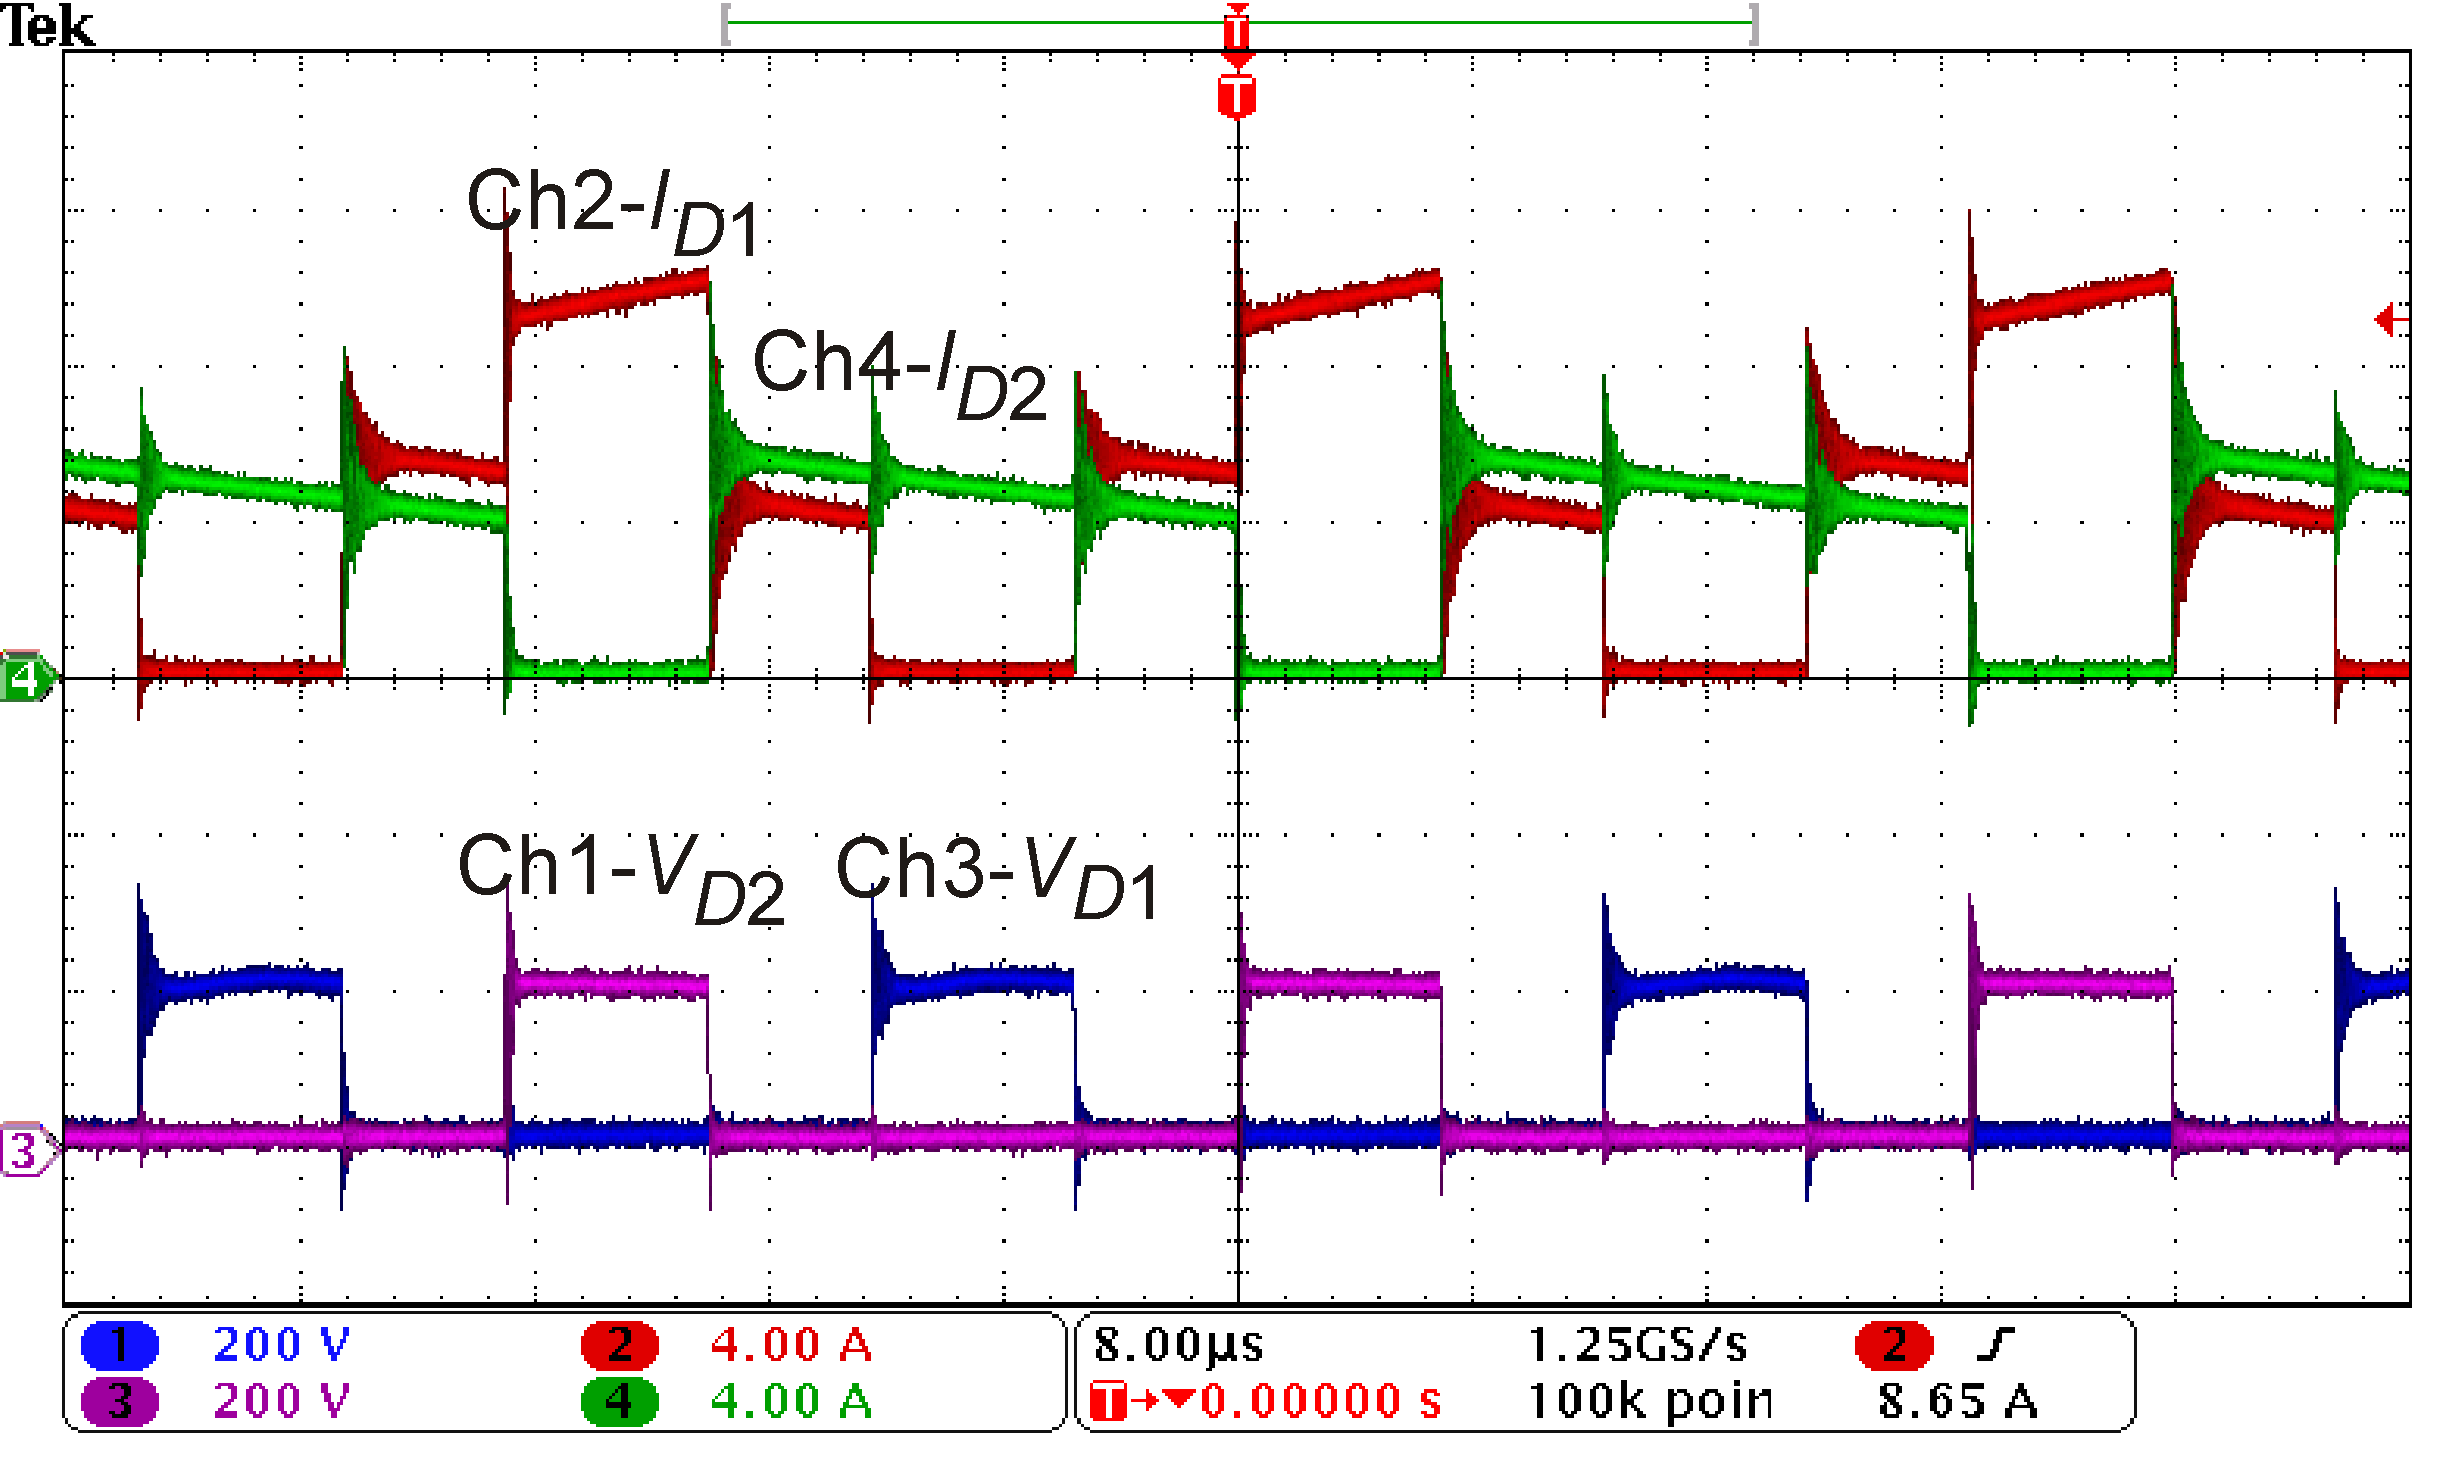
\includegraphics[width=0.7\linewidth]{../FIGURAS/Figuras_TFC_Eric/Formas_de_onda/Diodos_EGIBC}
	\fonte{Fonte: Pereira, D. C. (2019) \cite{denis}.}
	\label{pc_wav_0}
\end{figure}


\begin{figure}[!h]
	\centering
	\caption{Formas de onda para o estágio PC: Correntes (verde e vermelho) e tensões (azul e lilás) nos MOSFETs.}
	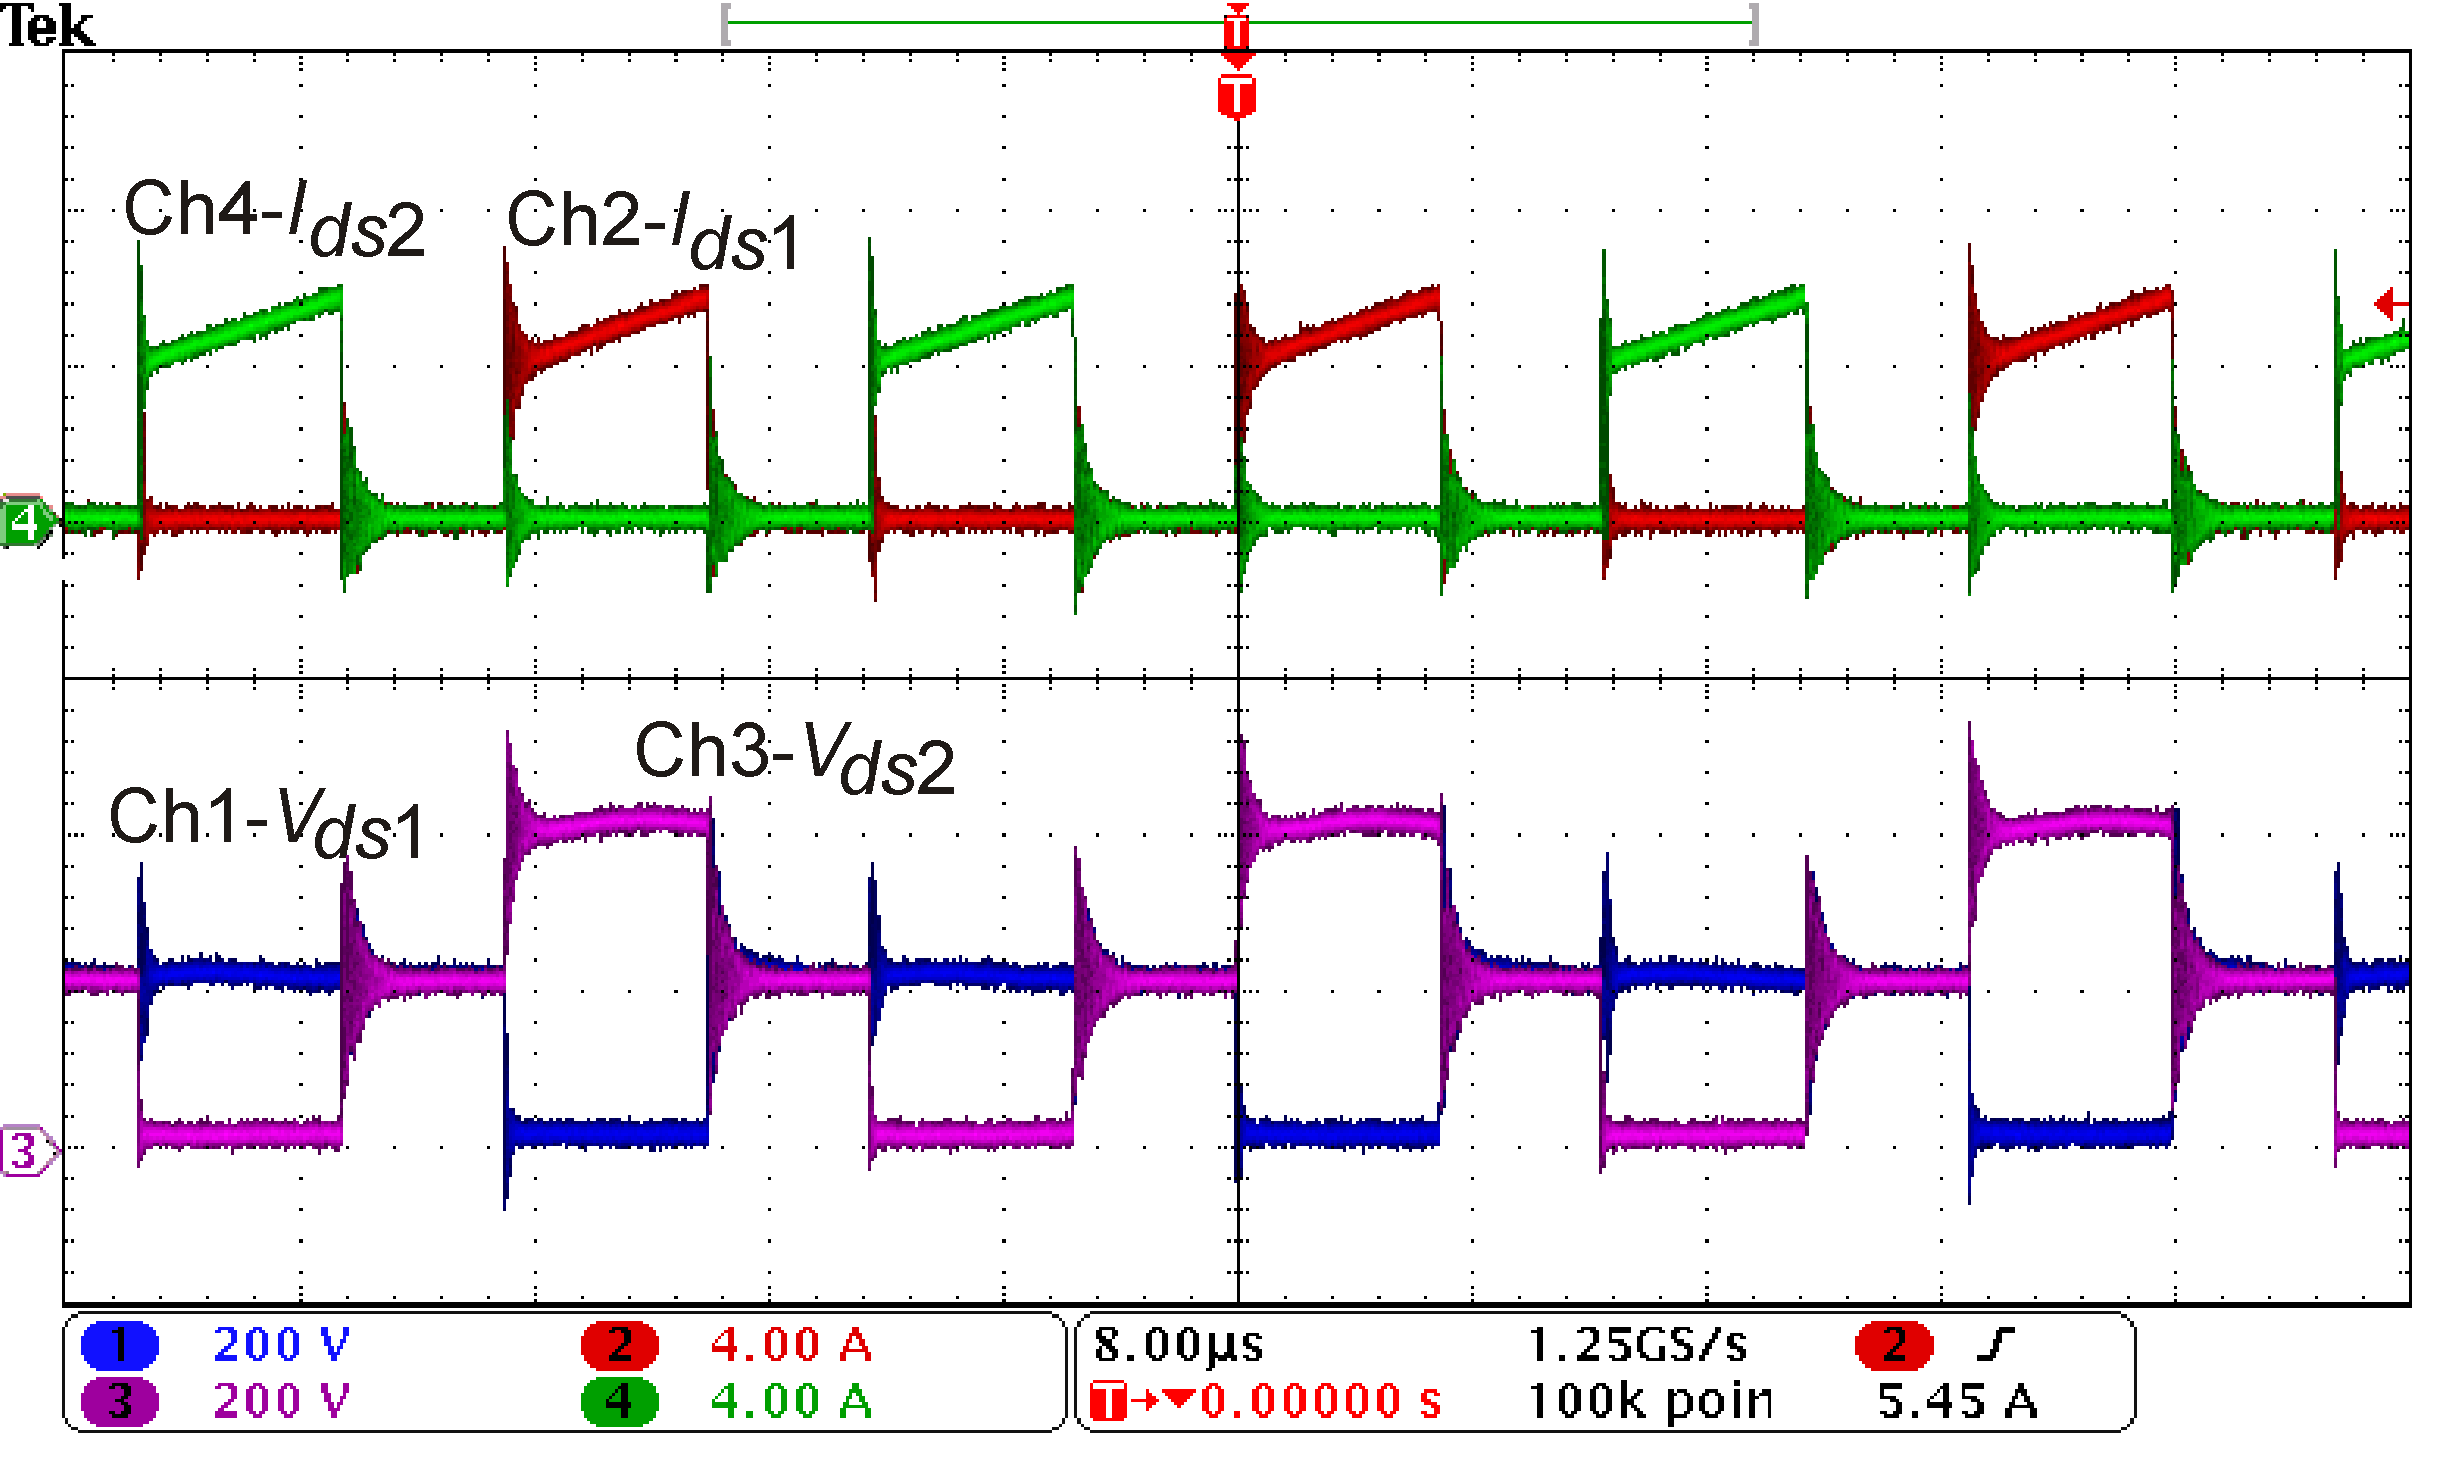
\includegraphics[width=0.7\linewidth]{../FIGURAS/Figuras_TFC_Eric/Formas_de_onda/MOSFETs_EGIBC}
	\fonte{Fonte: Pereira, D. C. (2019) \cite{denis}.}
	\label{pc_wav_1}
\end{figure}

\begin{figure}[!h]
	\centering
	\caption{Formas de onda para o estágio PC: Correntes (verde e vermelho) nos indutores e tensões de \textit{gate} dos MOSFETs (azul e lilás).}
	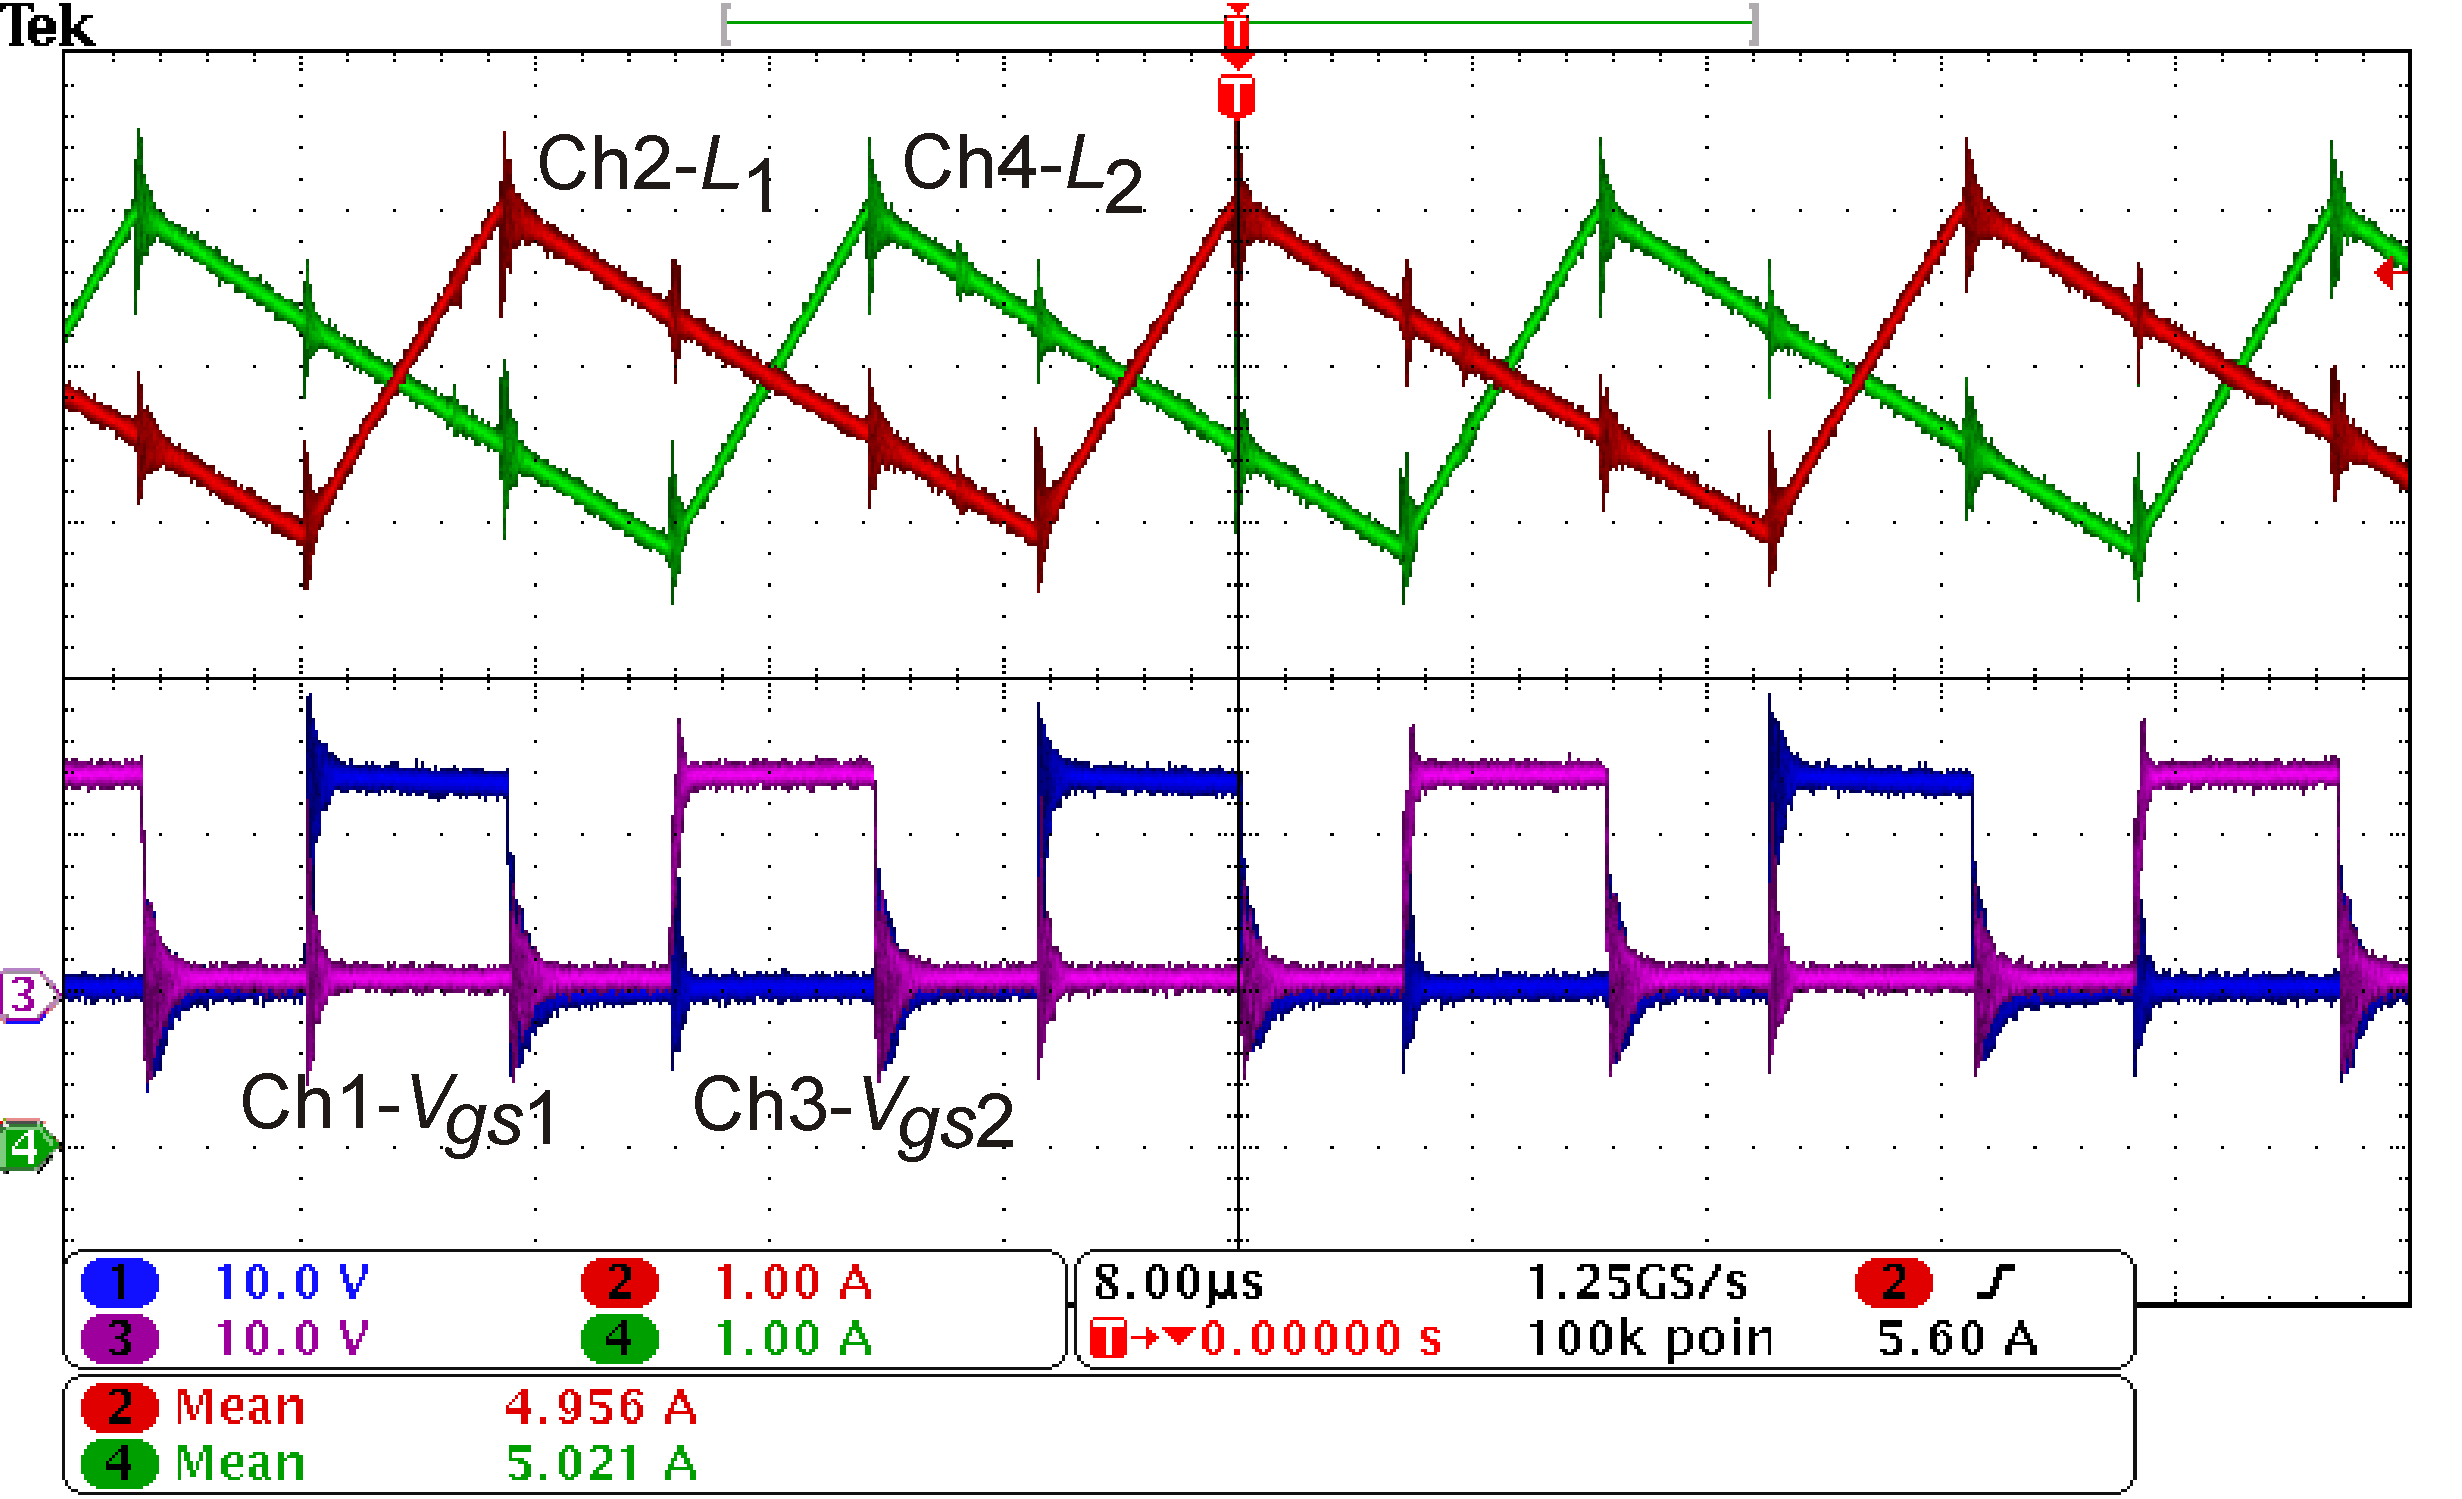
\includegraphics[width=0.7\linewidth]{../FIGURAS/Figuras_TFC_Eric/Formas_de_onda/Inductors_EGIBC}
	\fonte{Fonte: Pereira, D. C. (2019) \cite{denis}.}
	\label{pc_wav_88}
\end{figure}

Na figura \ref{pc_wav_2}, o conversor com os dois estágios é sujeito a um distúrbio de aproximadamente 10\% na tensão da rede. Constata-se que o erro em regime permanente é aproximadamente nulo e a saída retorna suavemente ao valor nominal.

%:controle
\begin{figure}[!h]
	\centering
	\caption{Formas de onda para o estágio PC: Distúrbio na tensão da rede. Corrente de entrada (vermelho), corrente de saída (verde), tensão de barramento (lilás) e tensão de saída (azul)}
	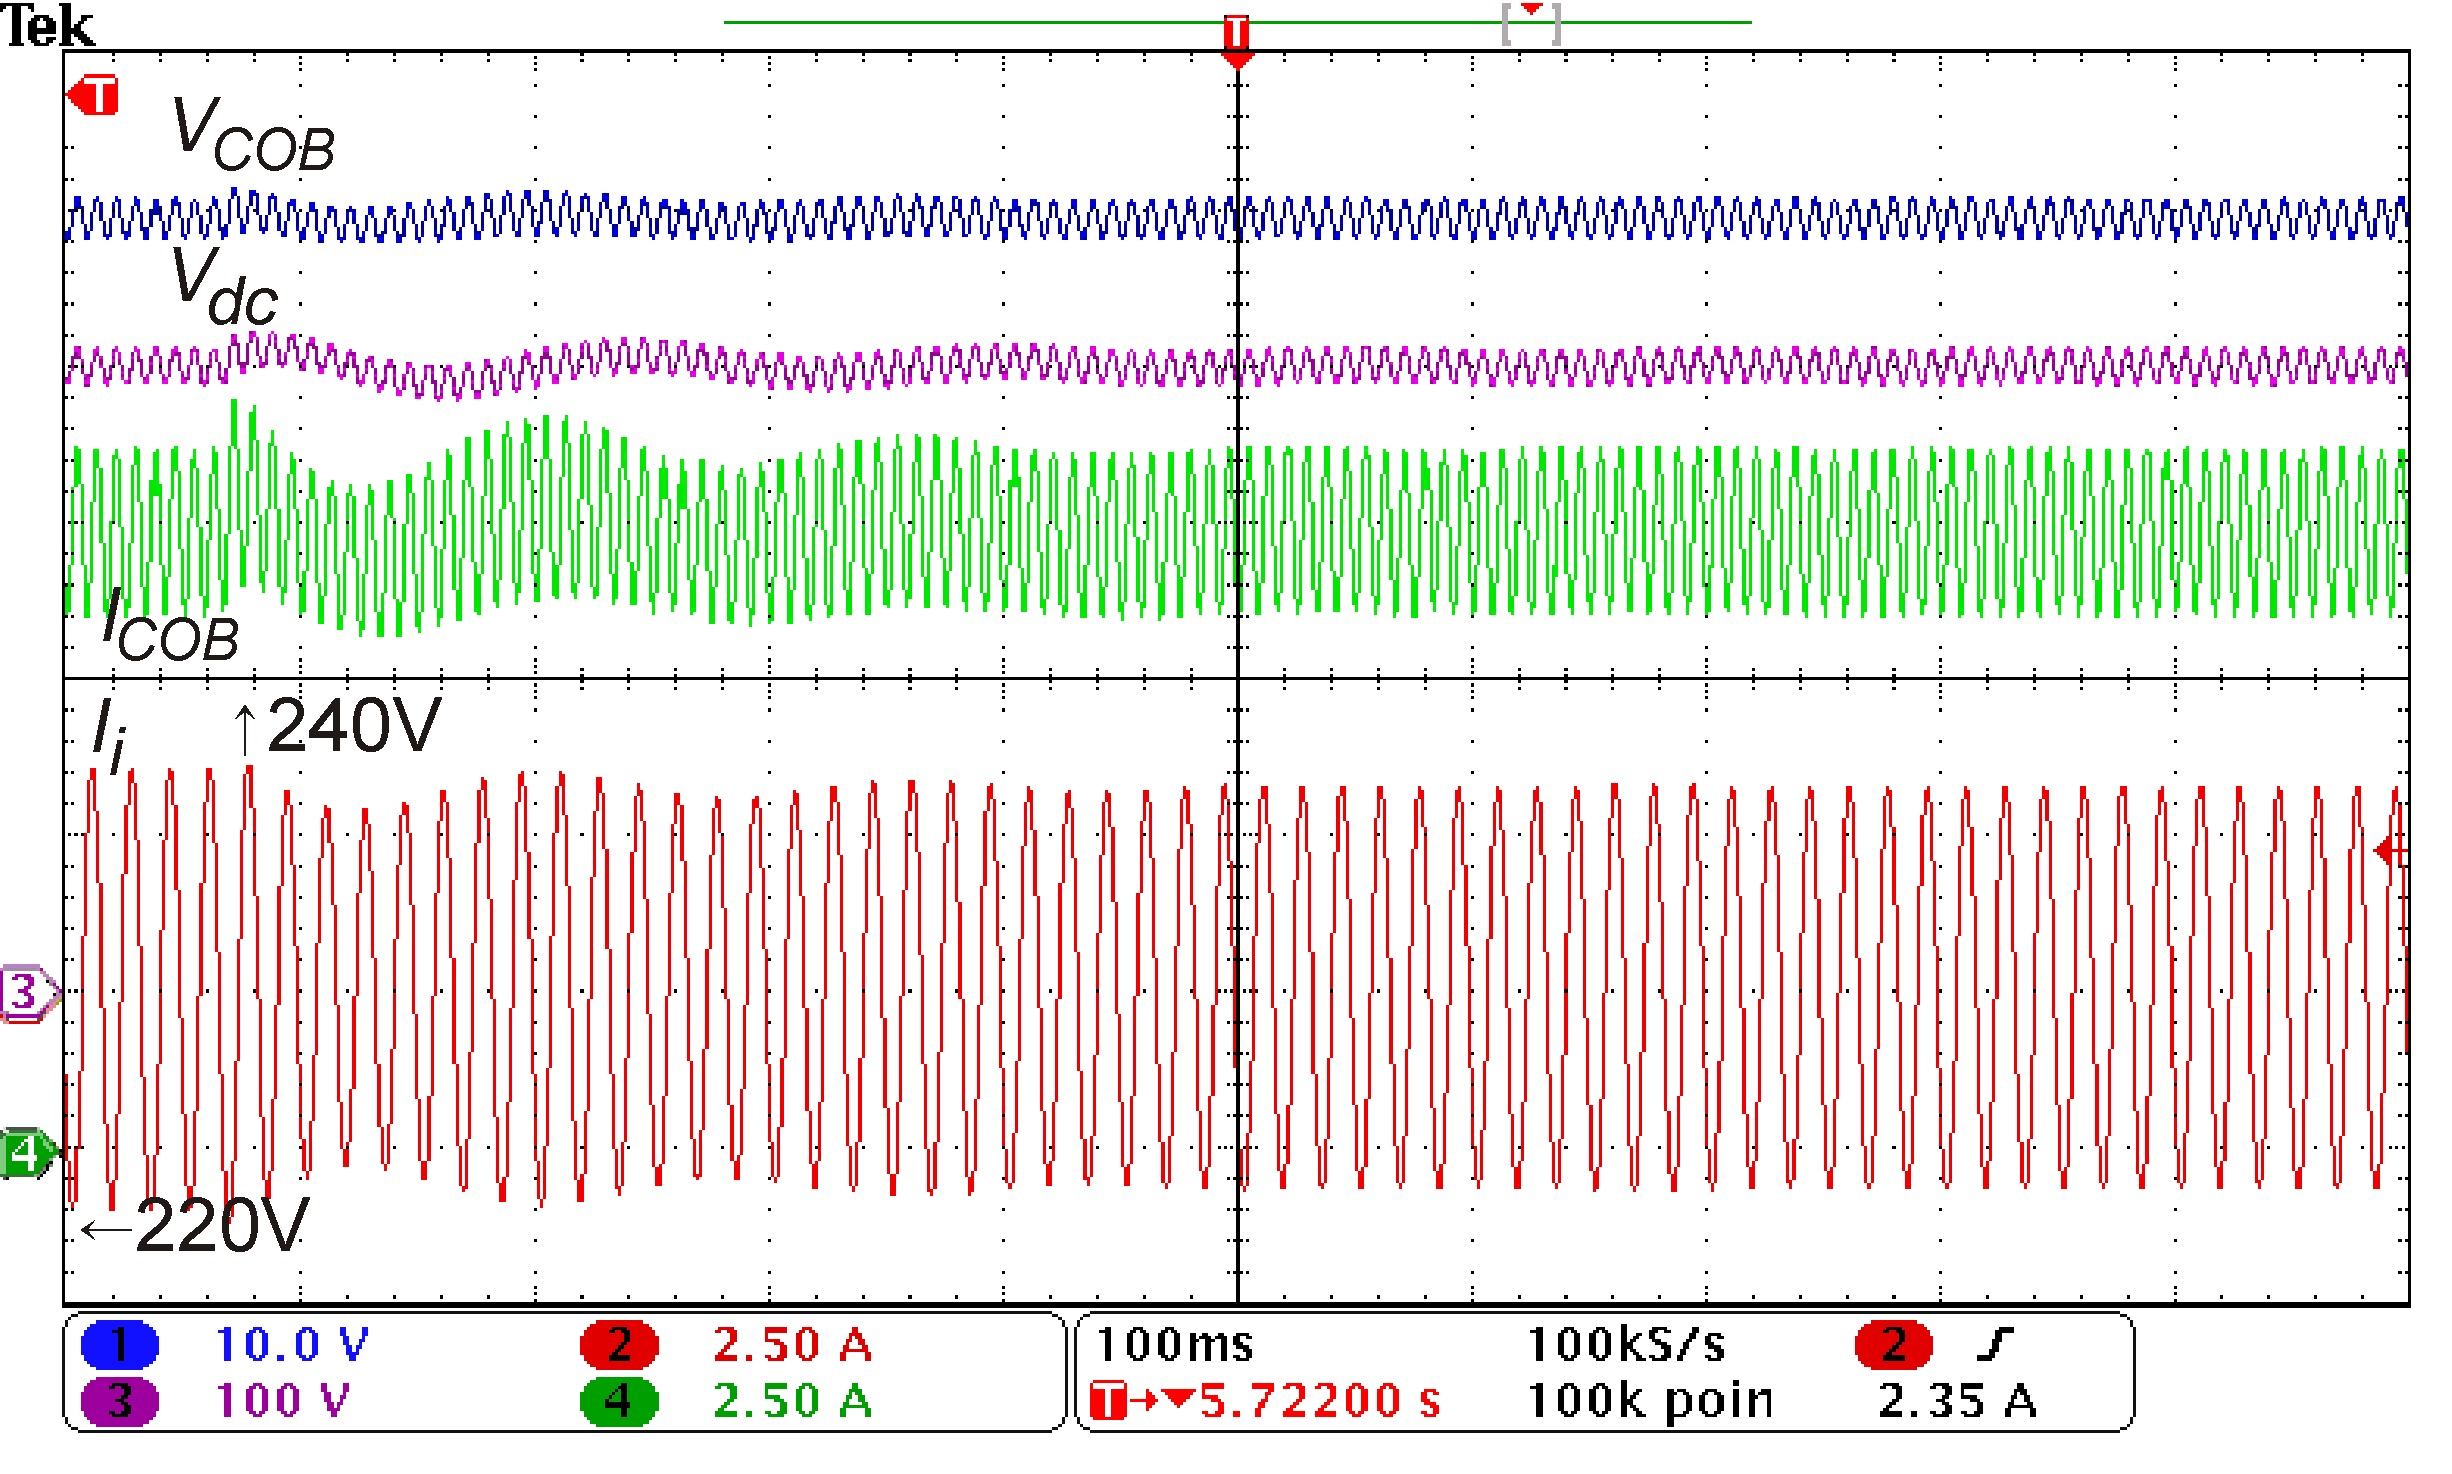
\includegraphics[width=0.7\linewidth]{../FIGURAS/Figuras_TFC_Eric/Formas_de_onda/Detailed_220V_to_240V}
	\fonte{Fonte: Pereira, D. C. (2019) \cite{denis}.}
	\label{pc_wav_2}
\end{figure}


A eficiência deste estágio foi medida em 94\%.




\section{Resultados gerais}

As placas referentes a este protótipo, tanto de potência quanto de controle quanto de acionamento, são apresentadas na figura \ref{pc_pfc_proto}.

\begin{figure}[!h]
	\centering
	\caption{Protótipo montado}
	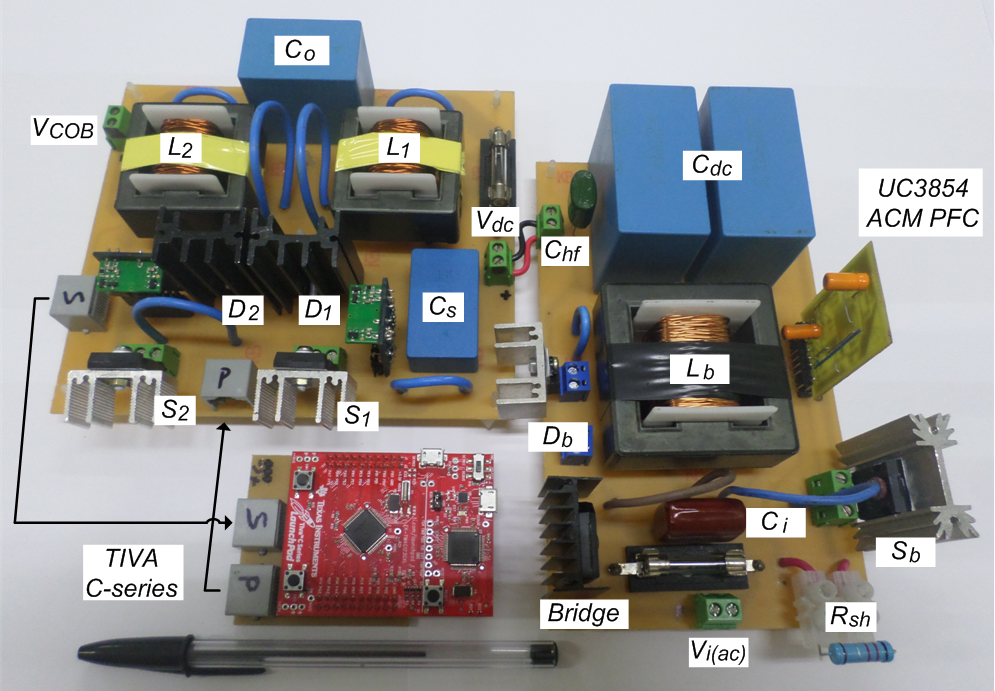
\includegraphics[width=0.7\linewidth]{../FIGURAS/Figuras_TFC_Eric/Figuras/Prototipo_ACM-EGIBC.png}
	\fonte{Fonte: Pereira, D. C. (2019) \cite{denis}.}
	\label{pc_pfc_proto}
\end{figure}

A eficiência do estágio PC na corrente nominal de 10 A foi medida em 94 \% e a do estágio PFC em 96\%, levando a uma eficiência global de 90\%. O fator de potência resultante foi de 0,99 e a distorção harmônica foi de 2,17\%.

Na figura \ref{tdh_super} é mostrada uma sobreposição das componentes harmônicas presentes na corrente de entrada com o máximo permitido segundo a norma IEC 61000-3-2 Classe C. Constata-se que a norma é atendida com margem mesmo sem filtro de harmônicas, graças ao controle PFC implementado.

\begin{figure}[!h]
	\centering
	\caption{Componentes harmônicas da corrente de entrada do conversor.}
	\includegraphics[width=0.7\linewidth]{../FIGURAS/Figuras_TFC_Eric/Figuras/iec61000-3-2_controlled_two-stage_pt}
	\fonte{Acervo Pessoal.}
	\label{tdh_super}
\end{figure}


\chapter{Considerações sobre atenuação ativa de ripple}

%Basicamente o último relatório do Braga.

Este é um pequeno equacionamento introdutório relativo a uma hipótese, sobre qual seria o efeito de se utilizar compensação ativa de \textit{ripple} no segundo estágio objetivando a redução da capacitância de barramento, técnica similar a \cite{guilherme} e \cite{bruno}, porém aqui a atenuação será feita sem degradação do fator de potência.


\section{Matemática}

%As próximas páginas foram geradas automaticamente a partir de um CAS, por isso a formatação está meio ruim. Os comentários podem estar meio vagos sem o código, apenas com as saídas. Caso o leitor resolva analisar mais a fundo, peço que solicite o arquivo original. 

Para a análise deste capítulo, o conversor será tratado não como dois, mas como três estágios, o PFC, o PC e um intermediário, que será chamado de ES, do inglês \textit{Energy Storage}.

%:conversor 3 estágios
\begin{figure}[!h]
	\centering
	\caption{Topologia multi-estágios adotada neste capítulo}
	\includegraphics[scale=.8]{../ESQUEMAS/treestage.png}\\
	\fonte{Acervo Pessoal.}
	\label{c}
\end{figure}

Nesta seção, serão deduzidas as expressões que descrevem o comportamento do conversor com compensação ativa de \textit{ripple}. O primeiro passo é equacionar a potência de entrada e a de saída no estágio de armazenamento de energia, representado pelo capacitor.

A potência fornecida pelo PFC é uma senóide ao quadrado, pois o conversor deve emular uma carga resistiva. A potência drenada pelo PC, por outro lado, será feita constante pelo controle do estágio de saída. Para o ES, portanto, teremos um fluxo de potência conforme a figura \ref{cs5_1}.

\begin{equation}
P_{in}(t):=2P\sin{(wt)}^2
\end{equation}

\begin{equation}
P_{out}(t):=P
\end{equation}

\begin{figure}[!h]
	\centering
	\caption{Fluxo de potência de entrada (azul) e saída (vermelho) no estágio ES}
	\includegraphics[width=.75\linewidth,height=.80\textheight,keepaspectratio]{../GRAFICOS/cs5_img/cs5_1}
	\fonte{Acervo Pessoal.}
	\label{cs5_1}
\end{figure}

Dessa forma, a energia no capacitor será:

\begin{equation}
E_{cap}( w,P,t) := \int{P_{in}(t)-P_{out}(t)dt}
\end{equation}

Ou:

\begin{equation}
E_{cap}( w,P,t) := E_{media}-\frac{P\sin{(2tw)}}{2w}
\end{equation}

Não há produção de energia, portanto esta deve ser estritamente positiva para qualquer instante de tempo. Assim, substituindo a fórmula da energia no capacitor e igualando a zero, pode-se calcular o capacitor crítico como:

\begin{equation}
E_{méd}( C,V_{méd}) :=\frac{C V_{mid}^2}{2}
\end{equation}


\begin{equation}
C( P,V_{méd},\omega) :=\frac{P}{V_{méd}^2 \cdot \omega}
\end{equation}

%\begin{equation}
%8.289319952702883{{10}^{-6}}
%\end{equation}

Para as especificações deste trabalho, e adotando uma potência de saída de 300W, a capacitância assim calculada é próxima de 8,3 $\mu F$.


Esse seria o caso de ambos os estágios terem a capacidade de elevar ou abaixar a tensão, mas há sérias desvantagens nisso. Nosso protótipo é um \textit{boost} seguido de um \textit{buck}, então restrições devem ser adicionadas.

O primeiro estágio, como dito, é um \textit{boost}. Portanto, a tensão de saída deve sempre ser superior a de entrada, sob pena de não haver condução. Equacionando a energia da mesma forma que na célula anterior, encontra-se a forma da tensão de barramento.

\begin{equation}
V_b( P,V_{méd},\omega,t,C) :=\sqrt{ V{méd}^2 -\frac{P sin(2t\omega)}{C\omega}}
\end{equation}

A tensão de entrada, retificada, vale:

\begin{equation}
Vin( V_{pk},w,t) :=| V_{pk}\,\sin{(\omega t)}|
\end{equation}

Igualando as duas, obtém-se:

\begin{equation}
\operatorname{C}\left( P,\mathit{Vpk},\mathit{Vmid},w,t\right) :=-\frac{P\,\sin{(2tw)}}{{{\mathit{Vpk}}^{2}}w\,{{\sin{(tw)}}^{2}}-{{\mathit{Vmid}}^{2}}w}\mbox{}
\end{equation}

É preciso maximizar a expressão anterior em relação ao tempo usando um método algébrico qualquer, a fim de obter o capacitor que garantirá que a tensão de entrada não exceda a de saída em nenhum instante.

%\begin{equation}
%\includegraphics[width=.95\linewidth,height=.80\textheight,keepaspect%ratio]{../GRAFICOS/cs5_img/cs5_2}\mbox{}
%\end{equation}

A seguir, na figura \ref{cs5_3}, são apresentadas as tensões de entrada e de saída com o capacitor calculado para o conversor adotado neste trabalho, aproximadamente 13 $\mu F$.

\begin{figure}[!h]
	\centering
	\caption{Tensão de entrada retificada, em azul, e de barramento, em vermelho}
	\includegraphics[width=.95\linewidth,height=.80\textheight,keepaspectratio]{../GRAFICOS/cs5_img/cs5_3}
	\fonte{Acervo Pessoal.}
	\label{cs5_3}
\end{figure}


A razão saída/entrada não é atípica. A faixa de ganho que o controle deve percorrer é essencialmente a mesma da operação analizada na seção 2.1, caso o capacitor seja escolhido com um valor não tão crítico.

% Resta saber se o 3854 lidará bem com isso. O psim diz que sim.

%\includegraphics[width=.95\linewidth,height=.80\textheight,keepaspectratio]{../GRAFICOS/cs5_img/cs5_4}\mbox{}

Da mesma forma, porém em perspectiva inversa, o estágio de saída é um abaixador. Temos que garantir que a tensão de saída será sempre menor que a de barramento. Igualando as duas, obtém-se:

\begin{equation}
\operatorname{C}\left( P,\mathit{Vo},\mathit{Vmid},w\right) :=-\frac{P}{\left( {{\mathit{Vo}}^{2}}-{{\mathit{Vmid}}^{2}}\right) w}\mbox{}
\end{equation}

%\begin{equation}
%8.420896459888642{{10}^{-6}}
%\end{equation}

Na figura \ref{cs5_5}, são apresentadas as tensões de barramento e de saída para uma capacitância de aproximadamente 8,4 $\mu F$.

\begin{figure}[!h]
	\centering
	\caption{Tensão de barramento, em azul, e de saída, em vermelho}
	\includegraphics[width=.95\linewidth,height=.80\textheight,keepaspectratio]{../GRAFICOS/cs5_img/cs5_5}
	\fonte{Acervo Pessoal.}
	\label{cs5_5}
\end{figure}

Termina-se, assim, com uma restrição essencial e mais duas decorrentes da topologia tratada neste trabalho. O capacitor mínimo de projeto deverá ser maior que a maior das restrições.

Por fim, deve ser feita uma consideração operacional. Permitir maior \textit{ripple} significa também submeter os componentes a um maior esforço.

No último gráfico, figura \ref{cs5_6}, é apresentado o \textit{ripple} em função do capacitor para o caso estudado.

\begin{figure}[!h]
	\centering
	\caption{\textit{Ripple} no barramento em função do capacitor adotado}
	\includegraphics[width=.95\linewidth,height=.80\textheight,keepaspectratio]{../GRAFICOS/cs5_img/cs5_6}
	\fonte{Acervo Pessoal.}
	\label{cs5_6}
\end{figure}

\section{Teste em simulação}

Foi feita no Psim uma simulação dos dois estágios em conjunto, a fim de verificar se a hipótese é válida.

\begin{figure}[!h]
	\centering
	\caption{Circuito de dois estágios simulado para constatação da atenuação ativa de \textit{ripple}.}
	\includegraphics[scale=.55]{../ESQUEMAS/PFCA_AND_PC}\\
	\fonte{Acervo Pessoal.}
	\label{PFCA}
\end{figure}

No primeiro estágio, foi simulado um conversor hipotético que convencionaremos chamar de PFC absoluto, o qual é capaz de drenar uma corrente perfeitamente senoidal e entregar a potência drenada ao barramento independente da tensão deste, cujo esquemático é dado em \ref{PFCA}. Já no estágio PC, a lei de controle foi alterada para uma com ganho infinito na frequência de ripple, o que caracteriza a técnica de controle ressonante \cite{ogata}. A função transferência usada é dada na equação \ref{ft_res}

\begin{equation}
G(s)=\frac{s^3\cdot 1.888e-1 +s^2\cdot 1.657e3 +s\cdot 1.859e6 +5.601}{s^3\cdot 1.000 +s^2\cdot 0.000 +s\cdot5.685e5 +0.000}
\label{ft_res}
\end{equation}


Seguem, assim, na figura \ref{ond2}, as formas de onda obtidas na simulação, para uma capacitância de barramento de $16\mu F$, ou 20\% do valor nominal.

\begin{figure}[!h]
	\centering
	\caption{Formas de onda simuladas para análise de atenuação ativa de \textit{ripple}. \textit{Grid} 1: Tensão no barramento, tensão no COB LED e tensão de entrada retificada. \textit{Grid} 2: corrente de entrada. \textit{Grid} 3: corrente no COB LED.}
	\includegraphics[scale=.65]{../GRAFICOS/ond2}\\
	\fonte{Acervo Pessoal.}
	\label{ond2}
\end{figure}

Para efeito de comparação, foi simulado o conversor \textit{boost} projetado neste trabalho, como indicado em \ref{cici}. As formas de onda obtidas nesta configuração são apresentadas na figura \ref{ond}.

\begin{figure}[!h]
	\centering
	\caption{Circuito de dois estágios simulado para constatação da atenuação ativa de \textit{ripple}.}
	\includegraphics[scale=.55]{../ESQUEMAS/PFC_AND_PC}\\
	\fonte{Acervo Pessoal.}
	\label{cici}
\end{figure}

\begin{figure}[!h]
	\centering
	\caption{Formas de onda simuladas para análise de atenuação ativa de \textit{ripple}. \textit{Grid} 1: Tensão no barramento, tensão no COB LED e tensão de entrada retificada. \textit{Grid} 2: corrente de entrada. \textit{Grid} 3: corrente no COB LED.}
	\includegraphics[scale=.65]{../GRAFICOS/ond}\\
	\fonte{Acervo Pessoal.}
	\label{ond}
\end{figure}


Constata-se que a forma geral das ondas é como o deduzido, embora os valores de oscilação apresentem divergência, possivelmente devido a não adequação do controle do primeiro estágio, que não foi projetado para lidar com oscilações dessa magnitude na tensão de barramento. Isso é algo que deve ser analisado com mais cuidado, sendo este um tema para futuros trabalhos que podem ser realizados a partir da análise introdutória desenvolvida nesta seção.



% Este é um primeiro passo. A comprovação ainda requer uma modelagem de sinais de estatura mediana, um projeto mais robusto de controlador e um tratamento mais apropriado do fluxo de potência. O eventual progresso será relatado futuramente.


\chapter{Conclusão}

Neste trabalho foi implementado um conversor de potência para uma carga de iluminação atípica, de baixa tensão e elevada corrente. O EHC COB LED em questão apresentou uma nova perspectiva para o trabalho, exigindo a combinação de técnicas típicas dos \textit{drivers} de iluminação comuns com características de conversores de potência mais elevada, como a separação em dois estágios e o uso do modo de operação CCM.

A definicão da topologia representou certo desafio, sendo necessário encontrar conversores que se adequassem aos requisitos. O projeto de ambos seguiu cursos distintos, sendo finalmente construídos e postos para funcionar juntos, tendo atingido o objetivo proposto no início.

%Colocar novamente os resultados encontrados e falar brevemente sobre eles:

O \textit{driver} proposto se mostrou uma boa alternativa para o acionamento e controle de EHC COB LEDs, sendo capaz de atender aos requisitos com nível de complexibilidade razoável, capaz de ser competitivo a nível industrial. O primeiro estágio implementado experimentalmente apresentou uma eficiência de 96\%, enquanto que, com o segundo estágio, obteve-se uma eficiência de 94\%. Finalmente, o protótipo final construído, operando para acionar o EHC COB LED, teve uma eficiência global de 90\%, cumprindo com o requisito inicial. As normas referentes à qualidade de energia e qualidade de iluminação também foram devidamente atendidas.


Como trabalhos futuros, é sugerida a pesquisa de técnicas capazes de maior eficiência, como comutação suave, a implementação de uma topologia isolada, para o caso que seja necessário, ou ainda a continuação do estudo sobre atenuação ativa de \textit{ripple}, com o desenvolvimento de um PFC absoluto.



%Cabou.


%Tem mais não.





























































































































%% ----------------------------------------------------------

%% ELEMENTOS POS-TEXTUAIS

\postextual

\begin{thebibliography}{99}

\bibitem{apollo} FLIP CHIP OPTO, “Apollo 600 datasheet”, 2016c. Disponível em: \cite{github}.

\bibitem{cie-foto} CIE, 2016. CIE TN 004:2016 - The Use of Terms and Units in Photometry – Implementation of the CIE System for Mesopic Photometry

\bibitem{cie-irc} CIE, 1995. CIE 13.3-1995 - Method of Measuring and Specifying Colour Rendering Properties of Light Sources

\bibitem{ieee-flicker} IEEE. “Recommended Practices for Modulating Current in High Brightness LEDs for Mitigating Health Risks to Viewers”. IEEE, Std. 1789, pp. 1-80, 2015.

\bibitem{liu} LIU, L. et al. “Thermal Analysis and Comparison of Heat Dissipation Methods on High Power LEDs”. Proc. of ICEPT-HDP 2010, pp. 1366–1370, Agosto 2010.

\bibitem{led-1} LOPES, S. B. “Eficiência Energética em Sistemas de Iluminação Pública.” Dissertação de Mestrado. Universidade de São Paulo. São Paulo, 2002.

\bibitem{led-2} POLONSKII, M.; SEIDEL, A. R. “Reatores Eletrônicos para Iluminação Fluorescente”. Editora Unijuí 1. ed. Ijuí, 2008.

\bibitem{led-3} DUPUIS, R.D.; KRAMES, M.R. "History, Development, and Applications of High-Brightness Visible Light-Emitting Diodes." Journal of Lightwave Technology, vol.26, no.9, pp.1154-1171, May, 2008.

\bibitem{schubert} SCHUBERT, E. F. “Light-Emitting Diodes”, Cambridge University Press, 2nd Edition, Cambridge, UK, 2006.

\bibitem{qoe} IEC. IEC 61000-3-2 – Electromagnetic Compatibility (EMC) Part 3-2: “Limits for Harmonics Current Emissions (equipment input current < 16 A per phase)”. International Electrotechnical Commision. 2005.

\bibitem{guilherme} SOARES, G. M. et al.; “Capacitance minimization in offline LED drivers using an active ripple-compensation technique”, IEEE Transactions on Power Electronics, vol. 32, nº 4, pp. 3022-3033, 2017.

\bibitem{sadiku} C. Alexander, M. N. O. Sadiku, Fundamentos de Circuitos Elétricos, 5a edição, McGrawHill, 2013.

\bibitem{guilherme-dissert} SOARES, G. M.; “Sistema Inteligente de Iluminação de Estado Sólido com Controle Remoto e Análise de Parâmetros da Rede Elétrica”. Dissertação de Mestrado. Universidade Federal de Juiz de Fora. Juiz de Fora, 2014.

\bibitem{hart} HART, D. W.; “Power Electronics”, McGraw-Hill Education, 2011.

\bibitem{on} ON, 2014. AND8123/D - Power Factor Correction Stages Operating in Critical Conduction Mode. Disponível em \cite{github}.

\bibitem{denis} PEREIRA, D. C.; “Diodos Emissores de Luz Integrados de Alta Corrente (EHC COB LEDs): Caracterização e Circuitos de Acionamento”. Universidade Federal de Juiz de Fora. Juiz de Fora, 2019.

\bibitem{uc3854} TEXAS INSTRUMENTS. “UC3854 High-Power Factor Pre-regulator”, 2016. Texas
Instruments Inc. Disponível em \cite{github}.

\bibitem{slua} TODD, P. C.; “UC3854 Controlled Power Factor Correction Circuit Design”. Unitrode Application Note, 1999. Disponível em \cite{github}.

\bibitem{bruno} Heleno, B. S.; “Controle Robusto Baseado em Desigualdades Matriciais Lineares Aplicado a um Conversor Integrado Buck-Boost Flyback para o Acionamento de LEDs com Entrada Universal”. Universidade Federal de Juiz de Fora. Juiz de Fora, 2019.

\bibitem{braga} Braga, H. A. C.; “Conversores Multiníveis em Corrente”. Universidade Federal de Santa Catarina. Santa Catarina, 1996.

\bibitem{artigo_do_china} LEE, O.; CHO, S. Y.; MOON, G. W.; “Interleaved Buck Converter Having Low Switching Losses and Improved Step-Down Conversion Ratio”. IEEE Transactions on Power Electronics, vol. 27, n. 8, pp. 3664-3675, 2012.

\bibitem{otro-bruno} ROSA, B. T.; “Pré-Regulador Boost Orientado ao Acionamento de LED COB”. Universidade Federal de Juiz de Fora. Juiz de Fora, 2017.

\bibitem{github} GITHUB.  \href{https://github.com/Pusiol/TFC/}{https://github.com/Pusiol/TFC/}.

\bibitem{ogata} OGATA, K. “Engenharia de Controle Moderno”, Ed. Pearson, 5ª ed., 2015.

\bibitem{acs} ALLEGRO. “Fully Integrated, Hall Effect-Based Linear Current Sensor IC with 2.1 kVRMS Isolation and a Low-Resistance Current Conductor”, Allegro Micro Systems, LLC, 2017. Disponível em \cite{github}.


\bibitem{livinha} MENDES, L. S. “Desenvolvimento de Plataforma Compacta para Prototipagem de Conversores de Potência”. Trabalho de Conclusão de Curso de Graduação, Universidade Federal de Juiz de Fora (UFJF), Faculdade de Engenharia Elétrica, 2018.


\end{thebibliography}













\end{document}
